\documentclass[whitelogo]{tudelft-report}
\usepackage{natbib}
\usepackage{changes}
\usepackage{float}
\graphicspath{{../images/}}
\begin{document}

%% Use Roman numerals for the page numbers of the title pages and table of
%% contents.
\frontmatter

%% Uncomment following 19 lines for a cover with a picture on the lower half only
%\title[tudelft-white]{Title}
% \subtitle[tudelft-cyan]{Optional subtitle}
% \author[tudelft-white]{J.\ Random Author}
% \affiliation{Technische Universiteit Delft}
% \coverimage{cover.jpg}
% \titleoffsetx{10cm}
% \titleoffsety{10cm}
% \afiloffsetx{1cm}
% \afiloffsety{18cm}
% \covertext[tudelft-white]{
%    \textbf{Cover Text} \\
%    possibly \\
%    spanning 
%    multiple 
%    lines
%    \vfill
%    ISBN 000-00-0000-000-0
% }
% \makecover

%% Uncomment following 16 lines for a cover with a picture on the lower half only
\title[tudelft-white]{Limit order placement optimization}
\subtitle[tudelft-black]{An attempt to understand cryptocurrency market event data using Reinforcement Learning techniques}
\author[tudelft-white]{Marc B. Juchli}
\affiliation{Technische Universiteit Delft}
\coverimage{tank.jpg}
\covertext[tudelft-white]{
    \textbf{Cover Text} \\
    possibly \\
    spanning 
    multiple 
    lines
    \vfill
}
%\setpagecolor{tudelft-cyan}
%\makecover[split]


%% Include an optional title page.
\begin{titlepage}


\begin{center}

%% Insert the TU Delft logo at the bottom of the page.

%% Print the title in cyan.
{\makeatletter
\largetitlestyle\fontsize{64}{94}\selectfont\@title
%\largetitlestyle\color{tudelft-cyan}\Huge\@title
\makeatother}

%% Print the optional subtitle in black.
{\makeatletter
\ifx\@subtitle\undefined\else
    \bigskip
   {\tudsffamily\fontsize{22}{32}\selectfont\@subtitle}    
    %\titlefont\titleshape\LARGE\@subtitle
\fi
\makeatother}

\bigskip
\bigskip

by
%door

\bigskip
\bigskip

%% Print the name of the author.
{\makeatletter
%\largetitlefont\Large\bfseries\@author
\largetitlestyle\fontsize{26}{26}\selectfont\@author
\makeatother}

\bigskip
\bigskip

to obtain the degree of Master of Science
%ter verkrijging van de graad van Master of Science

at the Delft University of Technology,
%aan de Technische Universiteit Delft,

to be defended publicly on Tuesday January 1, 2013 at 10:00 AM.
%in het openbaar de verdedigen op dinsdag 1 januari om 10:00 uur.

\vfill

\begin{tabular}{lll}
    Student number: & 1234567 \\
    Project duration: & \multicolumn{2}{l}{March 1, 2012 -- January 1, 2013} \\
    Thesis committee: & Prof.\ dr.\ ir.\ J.\ Doe, & TU Delft, supervisor \\
        & Dr.\ E.\ L.\ Brown, & TU Delft \\
        & Ir.\ A.\ Aaronson, & Acme Corporation
\end{tabular}
%% Only include the following lines if confidentiality is applicable.

\bigskip
\bigskip
\emph{This thesis is confidential and cannot be made public until December 31, 2013.}
%\emph{Op dit verslag is geheimhouding van toepassing tot en met 31 december 2013.}

\bigskip
\bigskip
An electronic version of this thesis is available at \url{http://repository.tudelft.nl/}.
%\\[1cm]

%\centering{
\includegraphics{cover/logo_black}}


\end{center}

\begin{tikzpicture}[remember picture, overlay]
    \node at (current page.south)[anchor=south,inner sep=0pt]{
        
\includegraphics{cover/logo_black}
    };
\end{tikzpicture}

\end{titlepage}



\chapter*{Abstract}
\setheader{Abstract}

\begin{abstract}
For various reasons, financial institutions often make use of high-level trading strategies when buying and selling assets.
Many individuals, irrespective or their level of prior trading knowledge, have recently entered the field of trading due to the increasing popularity of cryptocurrencies, which offer a low entry barrier for trading.
Regardless of the intention or trading strategy of these traders, the invariable outcome is their attempt to buy or sell assets. 
However, in such a competitive field, experienced market participants seek to exploit any advantage over those who are less experienced, for financial gain.
Therefore, this work aims to make a contribution to the important issue of how to optimize the process of buying and selling assets on exchanges, and to do so in a form that is accessible to other traders.

This research concerns the optimization of limit order placement within a given time horizon of 100 seconds and how to transpose this process into an end-to-end learning pipeline in the context of reinforcement learning.
Features were constructed from raw market event data that related to movements of the Bitcoin/USD trading pair on the Bittrex cryptocurrency exchange. These features were then used by deep reinforcement learning agents in order to learn a limit order placement policy.
To facilitate the implementation of this process, a reinforcement learning environment that emulates a local broker was developed as part of this work.
Furthermore, we defined an evaluation procedure which can determine the capabilities and limitations of the policies learned by the reinforcement learning agents and ultimately provides means to quantify the optimization achieved with our approach.

Our analysis of the results of this work includes the identification of patterns in cryptocurrency trading that were formed by market participants who posted orders, and a conceptual framework to construct data features containing these patterns.
We developed a fully-functioning reinforcement learning environment that emulates a local broker and, by means of this process, we identified which components are essential.
With the use of this environment, we were able to train and test multiple reinforcement learning agents whose aims were to optimize the placement of buy and sell limit orders.
During the evaluation, we were able to improve the parameter settings of the constructed reinforcement learning environment and therefore improve the policy learned by the agents.
Ultimately, we achieved a significant improvement in limit order placement with the application of a state-of-the-art deep Q-network agent and were able to simulate purchases and sales of 1.0 BTC at a price that was up to \$33.89 better than the market price.

We have made use of the OpenAI Gym\footnote{https://github.com/openai/gym} library and contributed our work to the community\footnote{https://github.com/backender/ctc-executioner} to enable further investigations to be carried out.
The work done in this thesis can be used as a framework to (1) build a component that acts as an intermediary between trader and exchange and (2) to enable exchanges to provide a new order type to be used by traders.
\end{abstract}

\chapter*{Preface}
\setheader{Preface}

Preface\ldots

\begin{flushright}
{\makeatletter\itshape
    \@author \\
    Delft, January 2013
\makeatother}
\end{flushright}



\tableofcontents

%% Use Arabic numerals for the page numbers of the chapters.
\mainmatter

\chapter{Introduction}
\label{chap:introduction}

Financial institutions make decisions to buy or sell assets for many reasons, including: customer requests, fundamental analysis\cite{fundamental-analysis}, technical analysis\cite{technical-analysis}, top-down investing\cite{td-investing}, and bottom-up investing\cite{bu-investing}.
High-level trading strategies oftentimes define how an institution positions itself in financial markets and, if applicable, towards its customers.
Regardless of the high-level trading strategy that is being applied, the invariable outcome is a decision to buy or sell assets.
This work aims to take a step towards answering the important question of how one can optimize a purchase or sale of an asset on a stock exchange with the use of reinforcement learning techniques.
The subsequent sections will elaborate this problem briefly and state the research objectives of this work.
We will list the contributions made to research communities throughout this work, followed by a brief overview of the structure of this report.

\section{Context and Problem Statement}
\label{sec:problem-statement}

We are concerned about the way assets, specifically \textit{securities} (exchange traded assets), are traded on stock exchanges.
There is little consensus as to when corporate stock was first traded; some argue that the exchange, in the form we know it today, dates back as far as 1531, when East Indian Company stock was traded in Antwerp\cite{stock-exchange}.
Modern financial markets such as the London Stock exchange (LSE), the New York Stock Exchange (NYSE), but also the numerous crypto-currency exchanges which have appeared suddenly in the last few years, all rely on the very same principles as back then.
They allow participants (called "traders") to buy or sell a given amount of a security at a particular price.
In the late 1990s, the regulatory authorities started to let traders access the markets using electronic communications networks (ECNs) and so a new era dawned \cite{patterson2012dark}.
Since then, high frequency trading (HFT) and sophisticated algorithmic trading vehicles have made up a substantial and ever-increasing part of electronic market participants.
Their servers are oftentimes located within exchanges and specialized computer networks have been constructed to provide millisecond-level advantage in the arbitrage of trades between exchanges.
Ever since, traders without such equipment and techniques have felt that they are at a disadvantage in such an environment \cite{patterson2012dark}.
While anything except trading through electronic channels would be unthinkable today, a certain gap still exists between trading companies that have fibre access to the exchanges or supporting algorithms and investors who do not.
As a result, investors are forced to take an initial loss into account when buying or selling securities, which they might not even be aware of.
In order to understand why these losses are incurred, we have to have a basic understanding of a so-called order book and how securities are bought at an exchange.

\begin{figure}[H]
    \centering
    \makebox[\linewidth]{
        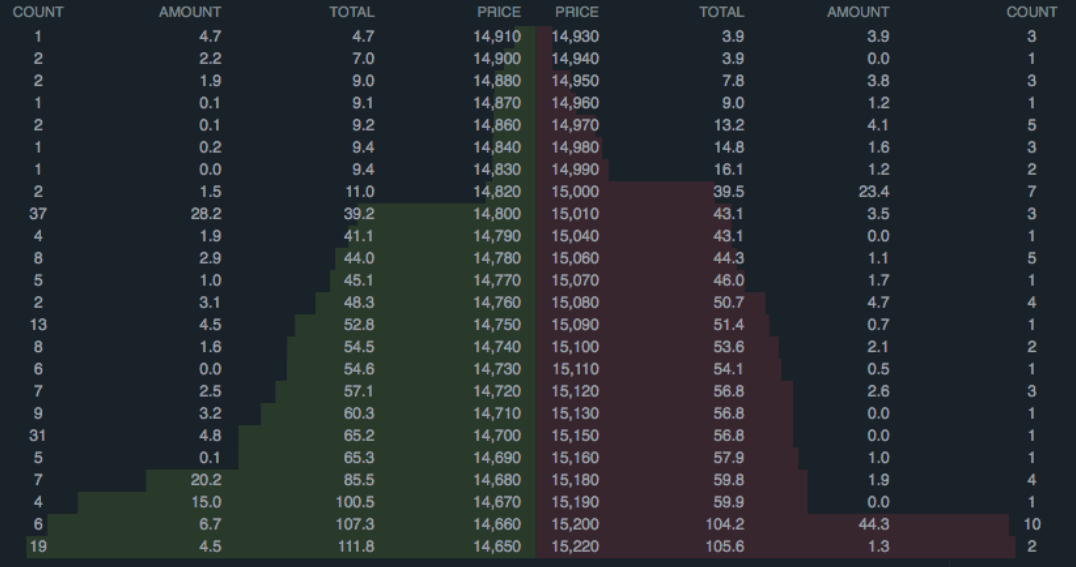
\includegraphics[width=12cm]{orderbook-gdax.png}
    }
    \caption{Order book snapshot: https://www.bitfinex.com/t/BTC:USD}
    \label{fig:intro-orderbook}
\end{figure}

Figure \ref{fig:intro-orderbook} shows a snapshot taken at some time $t$ of the trading pair Bitcoin (BTC) versus US dollar (USD) taken on the Bitfinex\footnote{https://www.bitfinex.com} cryptocurrency exchange.
The order book shows two columns, the parties who are willing to buy are on the left and the parties who are willing to sell are on the right.
The two columns indicate the number of buyers and sellers (\textit{count}) who are willing respectively to buy and sell a certain \textit{amount} for a given \textit{price}.
The column \textit{total} is the cumulative sum of the amount, or volume, on each side.
The difference between the figures in each column is the \textit{spread}.
In this particular case, the current best \textit{bid} price--at which someone is willing to buy--is \$14,910.00 and the best ask-price at which someone is willing to sell, is \$14,930.00.
Therefore, the spread is currently \$20.00.
\\
\\
Suppose we want to buy 1.0 BTC.
Two possible ways to do so are:
\begin{enumerate}
    \item Buy 1.0 shares immediately for \$14,930.00 from a seller. To do so, we submit a \textit{market} order.
    \item State a price at which we are willing to buy 1.0 shares at price $p$, for example at \$14,910.00, and wait until someone is willing to sell at this price. To do so, we submit a \textit{limit} order.
\end{enumerate}

Both types of orders come with their advantages and disadvantages.
A market order ensures that we will be able to acquire the stated amount of shares immediately for \$14'930.00, provided that no one else  has a prior claim to them and that the seller does not cancel his/her listing.
In this case, we are automatically willing to pay the next available best price.
However, we do pay a premium compared to the limit order since ask prices are listed higher than bid prices and the more shares one wants to buy, the more sellers we have to contact and accept their offers at an increased price.
With a limit order, the exchange guarantees that we will pay \$14,910.00 or less.
That is, when a seller is willing to sell for the stated price or less, the exchange will match the offers of both parties.
However, this comes with the risk that we will never be able to buy if nobody is going to sell at the demanded price, and this will force us to buy the shares demanded at a later point in time.
As the price of a share evolves over time, we might get lucky and be able to buy at a cheaper price than at the time of the initial attempt.
The other scenario is that the price did not develop in our favour such that we have to buy at a higher price later on; thus, we pay a so-called \textit{opportunity cost}.
A third order type, the \textit{cancel} order, allows a trader to cancel his/her previously posted limit or market order at any given point in time.
%Ultimately, we have a brief understanding of what traders are allowed to do at a stock exchange.
%We will now elaborate briefly how such a relatively simple concept of an order book and three types of orders can lead to a diverse range of situations a trader can find himself whereas at times this may be beneficial for his intentions and at times it will lead to paying a premium.
%If a seller realizes that we are about to buy for price $p$ at which is was willing to sell, he then could \textit{cancel} his offer as his incentive is to sell for a higher price.
%Perhaps this has been his/her intention to only post an offer but withdrawal as soon as a counter-offer will be listed that is close to his/her price.
%This method is known as \textit{quote stuffing}.

With this brief understanding of how traders can interact with the exchange, we can define the problem of \textit{order placement} as follows.
Order placement determines the price at which a trader places its order.
The aim of optimizing order placement are to minimize the opportunity cost and, ideally, achieve a more favorable price payable (or receive) than what is currently being offered at the market price.
Literature therefore specifies a time scale of from ten to one hundred seconds within which a trader has to complete his task of either buying or selling the shares \cite{guo2013optimal}.
A time scale of less than ten seconds applies in high frequency trading and one of above 100 seconds is known as \textit{order execution optimization}.
Thus, could we define order placement optimization as the price $p$ at which one should attempt to buy or sell $i$ shares within a time horizon $H$ of 100 seconds?
As we shall see, optimizing placement is not as trivial as one might think, even though the concepts of the order book and the three order types a trader can choose from are admittedly simple.
There are various properties in a limit order book, as well as the behaviour of the market participants, that changes over time.
All of which can drastically interfere with the intention of buying and selling.
Furthermore, since the foundation of electronic trading networks and algorithmic trading, the amount and sophistication of other market participants has been ever-increasing, with everyone aiming for an advantage over others.
%However, the prices for some financial products, including crypto-currencies, are very volatile such that it is likely to be able to buy for less than what is offered at the mentioned time $t$.
%In addition, there might be buyers and sellers in the near future which would consume our order.
%Thus, placing orders \textit{deeper} in the book and wait could be beneficial.
%
%According to Guo et. al. \cite{guo2013optimal} algorithmic trading is based on two different time scales: \textit{order execution} concerns about optimally slicing big orders into smaller ones in order to minimize the \textit{price impact}, that is, on a daily or weekly basis.
%\textit{Order placement} on the other hand concerns about optimally placing orders within ten to hundred seconds.
%In this thesis we are concerned about the latter, which conforms the context of the problem:

The fact that reinforcement learning functions by maximizing rewards makes this technique unarguably suitable in this context.
That is, how to place orders according to the given market condition and therefore protect an investor form paying the aforementioned premium to other participants in the market.
Ideally, such a learner will be able to foresee short-term trend changes such that the investor ultimately benefits from a better price at which to buy or sell the asset. 

\section{Research objectives}
\label{sec:intro-rq}

This work extends the findings of Kearns et. al. who have studied the behavior of order placement and order execution\cite{nevmyvaka2005electronic}, and developed a reinforcement learning strategy\cite{nevmyvaka2006reinforcement} for the purposes of optimization.
Their work explains how features derived from order book data were pre-processed and applied to a reinforcement learning algorithm which is similar to Q-Learning.
In this thesis, rather than constructing features by hand, we will describe a particular instance of how deep reinforcement learning techniques were employed in order to benefit from patterns in raw market data.
In addition, the cryptocurrency domain was chosen, instead of the traditional stock market.
Furthermore, while the previously mentioned work of Kearns et al. had success in using pre-processed market data as features, we believe that raw market data in combination with deep reinforcement learning can be equally successful.
Hence, our ambition is to determine if deep reinforcement learning is perhaps an even more suitable choice in order to deal with unexpected market situations.
Therefore we have formulated the following research question to be answered in this thesis:
\\
\\
\textbf{RQ 1:} How can the application of deep reinforcement learning contribute to the optimization of limit order placement?
%\textbf{RQ 1 (B):} Which cryptocurrency market events enable us to foresee opportunities to place limit orders at a favorable price with the use of deep reinforcement learning?
\\
\\
\textit{We chose to divide the research question into sub-questions as this follows the logical structure of this document and provides an understanding of the steps taken in order to give an answer to the main research question.}

\begin{quote}
\begin{description}
    \item[RQ 1.1:] Which historical market data patterns drive market participants to buy or sell assets, and how can these patterns be incorporated into features used by a deep reinforcement learning agent?
\end{description}
    Traders participating in financial markets, including cryptocurrency markets, can submit and cancel orders to trade shares.
    These events are recorded by the cryptocurrency exchange and are publicly accessible as raw market data.
    We intend to find patterns in the data which reflect the behavior of these market participants.
    The patterns found will form the basis of hypotheses suggesting that some behavioral patterns are more likely to lead traders either to buy or sell an asset in the short term.
    Whenever a hypothesis is true, one can determine a favorable price at which to buy or sell the asset, and hence, mitigate the impact of the order placement problem.
    Thus, we have to determine how to shape historical market data and construct features with the patterns found and incorporated that enable deep reinforcement learning agents to learn an order placement strategy.

\begin{description}
    \item[RQ 1.2:] How can one design a reinforcement learning environment and agents, in the context of order placement?
\end{description}
    In order to simulate and understand the outcome of order placement and, more importantly, build a reinforcement learning environment that allows interaction with agents, this work will suggest a way of translating the given problem into a reinforcement learning context.
    Consequently, we are required to build a framework which should provide collection and market data processing capabilities in order to reproduce a historical order book that serves as a data source.
    Further, we require that the framework provide the functionality of a match engine which emulates the functionality of a stock exchange that can match orders and determine the resulting price paid (or received) according to the historical order book.
    Ultimately, a reinforcement learning environment should be built to simulate and evaluate order placement.
    The environment should allow direct user interaction in order to place orders on demand and allow interaction with agents which act as intelligent traders.
    Therefore, we have made use of the OpenAI Gym\footnote{https://github.com/openai/gym} library and we contribute our work to the community to enable further investigations to be carried out.
    
    Further, we shall then build two reinforcement learners which will both act as intelligent traders and thereby place limit orders that provide an incentive to buy or sell an asset at a favorable price.
    Both agents should be driven by an end-to-end learning process by which the agent improves based on the outcome of the orders placed and ultimately learns a strategy for  buying and selling shares at favorable prices.
    The former agent is an adaptation of the well- known Q-Learning algorithm and optimizes only in accordance with the amount of assets to buy or sell and the given time horizon.
    This agent is a deep reinforcement learning agent that makes use of a convolutional neural network in order to detect patterns in market data.

\begin{description}
    \item[RQ 1.3:] How can one evaluate a reinforcement learning environment and agent in the context of order placement?
\end{description}
    The ability to quantify the capabilities of a limit order placement strategy learned by a reinforcement learning agent is of significant importance when answering the main research question in this thesis.
    Since there is no literature available which states results for the exact same data set, nor for any data set within the crypto- currency domain, a procedure has to be introduced by which different learning approaches and features considered can be evaluated.
    Therefore a measure is to be taken that is well-suited to the determination and comparison of the capabilities of a reinforcement learning agent in the order placement context.
    Furthermore, the evaluation procedure should identify the extent to which a limit order placement can be optimized in a given historical data set.
    As a result, the evaluation shall serve as a reliable measure of how well a learned order placement strategy performs.
    
\begin{description}
    \item[RQ 1.4:] In which way do the previously constructed features enable a reinforcement learning agent to improve the way it places orders?
\end{description}

    The significance of deep reinforcement learning and the use of features derived from market data has to be determined in the application of order placement.
    The findings shall be compared to the performance achieved by a learner which has less information available, as well as the previously identified limitations of the market data available.
    Finally, the limitations of a learned strategy are to be identified.
\end{quote}

\section{Document structure}

In Chapter \ref{chap:preliminaries}, we first provide background information to the reader on the components of a stock exchange. %and the fundamentals of the closely related time series.
Further, we make the reader familiar with (Deep) Reinforcement Learning.
In Chapter \ref{chap:related-work}, we elaborate on the behavior of order placement followed by approaches of both statistical and machine learning nature.
Chapter \ref{chap:data} explains the process of data collection and preparation which was carried out prior to its use in the subsequent chapters.
Chapter \ref{chap:setup} explains the experimental setup of the reinforcement learning environment, the agents and the way processed features are used.
In Chapter \ref{chap:analysis}, we analyze the data, carry out order placement, and include reasons for our findings.
Finally, in Chapter \ref{chap:discussion}, we formulate a conclusion of our findings and state a future research direction.

\chapter{Preliminaries}
\label{chap:preliminaries}

\section{Order Book}

Despite the fact that some of the participants in the market tend to gain a slight advantage over others (see Section \ref{sec:problem-statement}), without these highly active trading participants (also known as \textit{liquidity traders}) the market would suffer from the absence of liquidity.
The offerings are thereby listed in a \textit{limit order book} indicating the will to buy and sell a given asset for a certain price.
This section introduces the most popular order types and explains the characteristics of a limit order book.
We further show how participants can list their orders to appear in the book.

\subsection{Orders}
\label{sec:orders}

As indicated by the name, an order is an order to buy or sell a stock.
There are various types of orders which determine how the order that is placed should be executed on the broker side.
In this section we provide information about the two most common types, namely the \textit{limit order} and the \textit{market order},
We define the indication on whether to buy or sell as the \textit{Order Side},
\begin{equation}\label{eq:order-side}
    OrderSide=\{Buy, Sell\}
\end{equation}
\\
Before we define the order types in greater detail, we conclude what is said above and define the \textit{Order} as,
\begin{equation}\label{eq:order}
Order=\{Order_{Limit}, Order_{Market}\}
\end{equation}

\subsubsection{Limit order}
\label{sec:limit-order}

A limit order implies the attempt to buy or sell a stock at a specific price or better,
\begin{equation}\label{eq:order-limit}
    Order_{Limit}=\{side, quantity, price_{Limit}\}
\end{equation}
, where $side \in OrderSide$, $quantity \in \mathbb{R^+}$ and $price_{Limit} \in \mathbb{R^+}$.
\\
\\
A buy limit order can only be executed at the limit price or lower, and a sell limit order can only be executed at the limit price or higher \cite{sec-limit-order}.
More precisely, in case of a buy order and if the best price on the opposing side of the book becomes lower or equals (respectively higher or equals, in case of a sell order), the broker will match those two orders, resulting in a \textit{trade}.
The disadvantage of this order type is that there is no guarantee whether the order gets executed.
In case no order on the opposing side appears, the order remains (possibly forever) unexecuted.

\subsubsection{Market order}
\label{sec:market-order}

A market order implies the attempt to buy or sell a stock at the current market price, expressing the desire to buy (respectively sell) for the best available price. Therefore,
\begin{equation}
Order_{Market}=\{side, quantity\}
\end{equation}
, where $side \in OrderSide$ and $quantity \in \mathbb{R^+}$.
\\
\\
The advantage of a market order is that as long as there are willing buyers and sellers, the execution of the order is almost always guaranteed. \cite{sec-market-order}
The disadvantage is the price you pay when your order is executed.
Market orders are executed by starting from the best price of the opposing side, then traversing down the book as liquidity is consumed. 
Hence, market orders tend to become expensive, especially for large orders.

\subsection{Characteristics}
\label{sec:ob-characteristics}

Figure \ref{fig:intro-orderbook} shows a real world example of a limit order book; in this case the snapshot was taken from a known crypto-currency exchange.
Being precise, this is the \textit{state} of an order book at some time $t$ and shows the current offerings (in form of limit orders, see \ref{sec:limit-order}) from participants at this moment in time (we neglect the possibility that the state might have been changed during the data sending process). 
Hence, we refer to it as an \textit{order book state (OS)} and the \textit{order book (OB)} itself is defined as a set of order book states.
\begin{equation}\label{eq:order-book}
OB=\{OS_1, ... OS_n\}
\end{equation}
As we can see, every such state holds entries on the buyer and seller side which change in their \textit{price} and \textit{amount}.
To each such row, which can be formed by participants who submitted limit orders of some amount at the same price level, we refer to as \textit{order book entry ($OE_{s_l}$)} of the side $s$ at level $l$.
\begin{equation}
OE_{s_l}=\{count, price, amount\}
\end{equation}
, whereas $count \in \mathbb{N}$, $price \in \mathbb{R^+}$ and $amount \in \mathbb{R^+}$.
As a result, the order book state is a set containing order book entries for each \textit{side} (buy and sell) and a time stamp $ts$ of the state,
\begin{equation}\label{eq:order-book-state}
OS=\{ts, OE_{b_1}, ..., OE_{b_n}, OE_{s_1}, ..., OE_{s_n}\}
\end{equation}
\\
\begin{figure}[H]
    \centering
    \makebox[\linewidth]{
        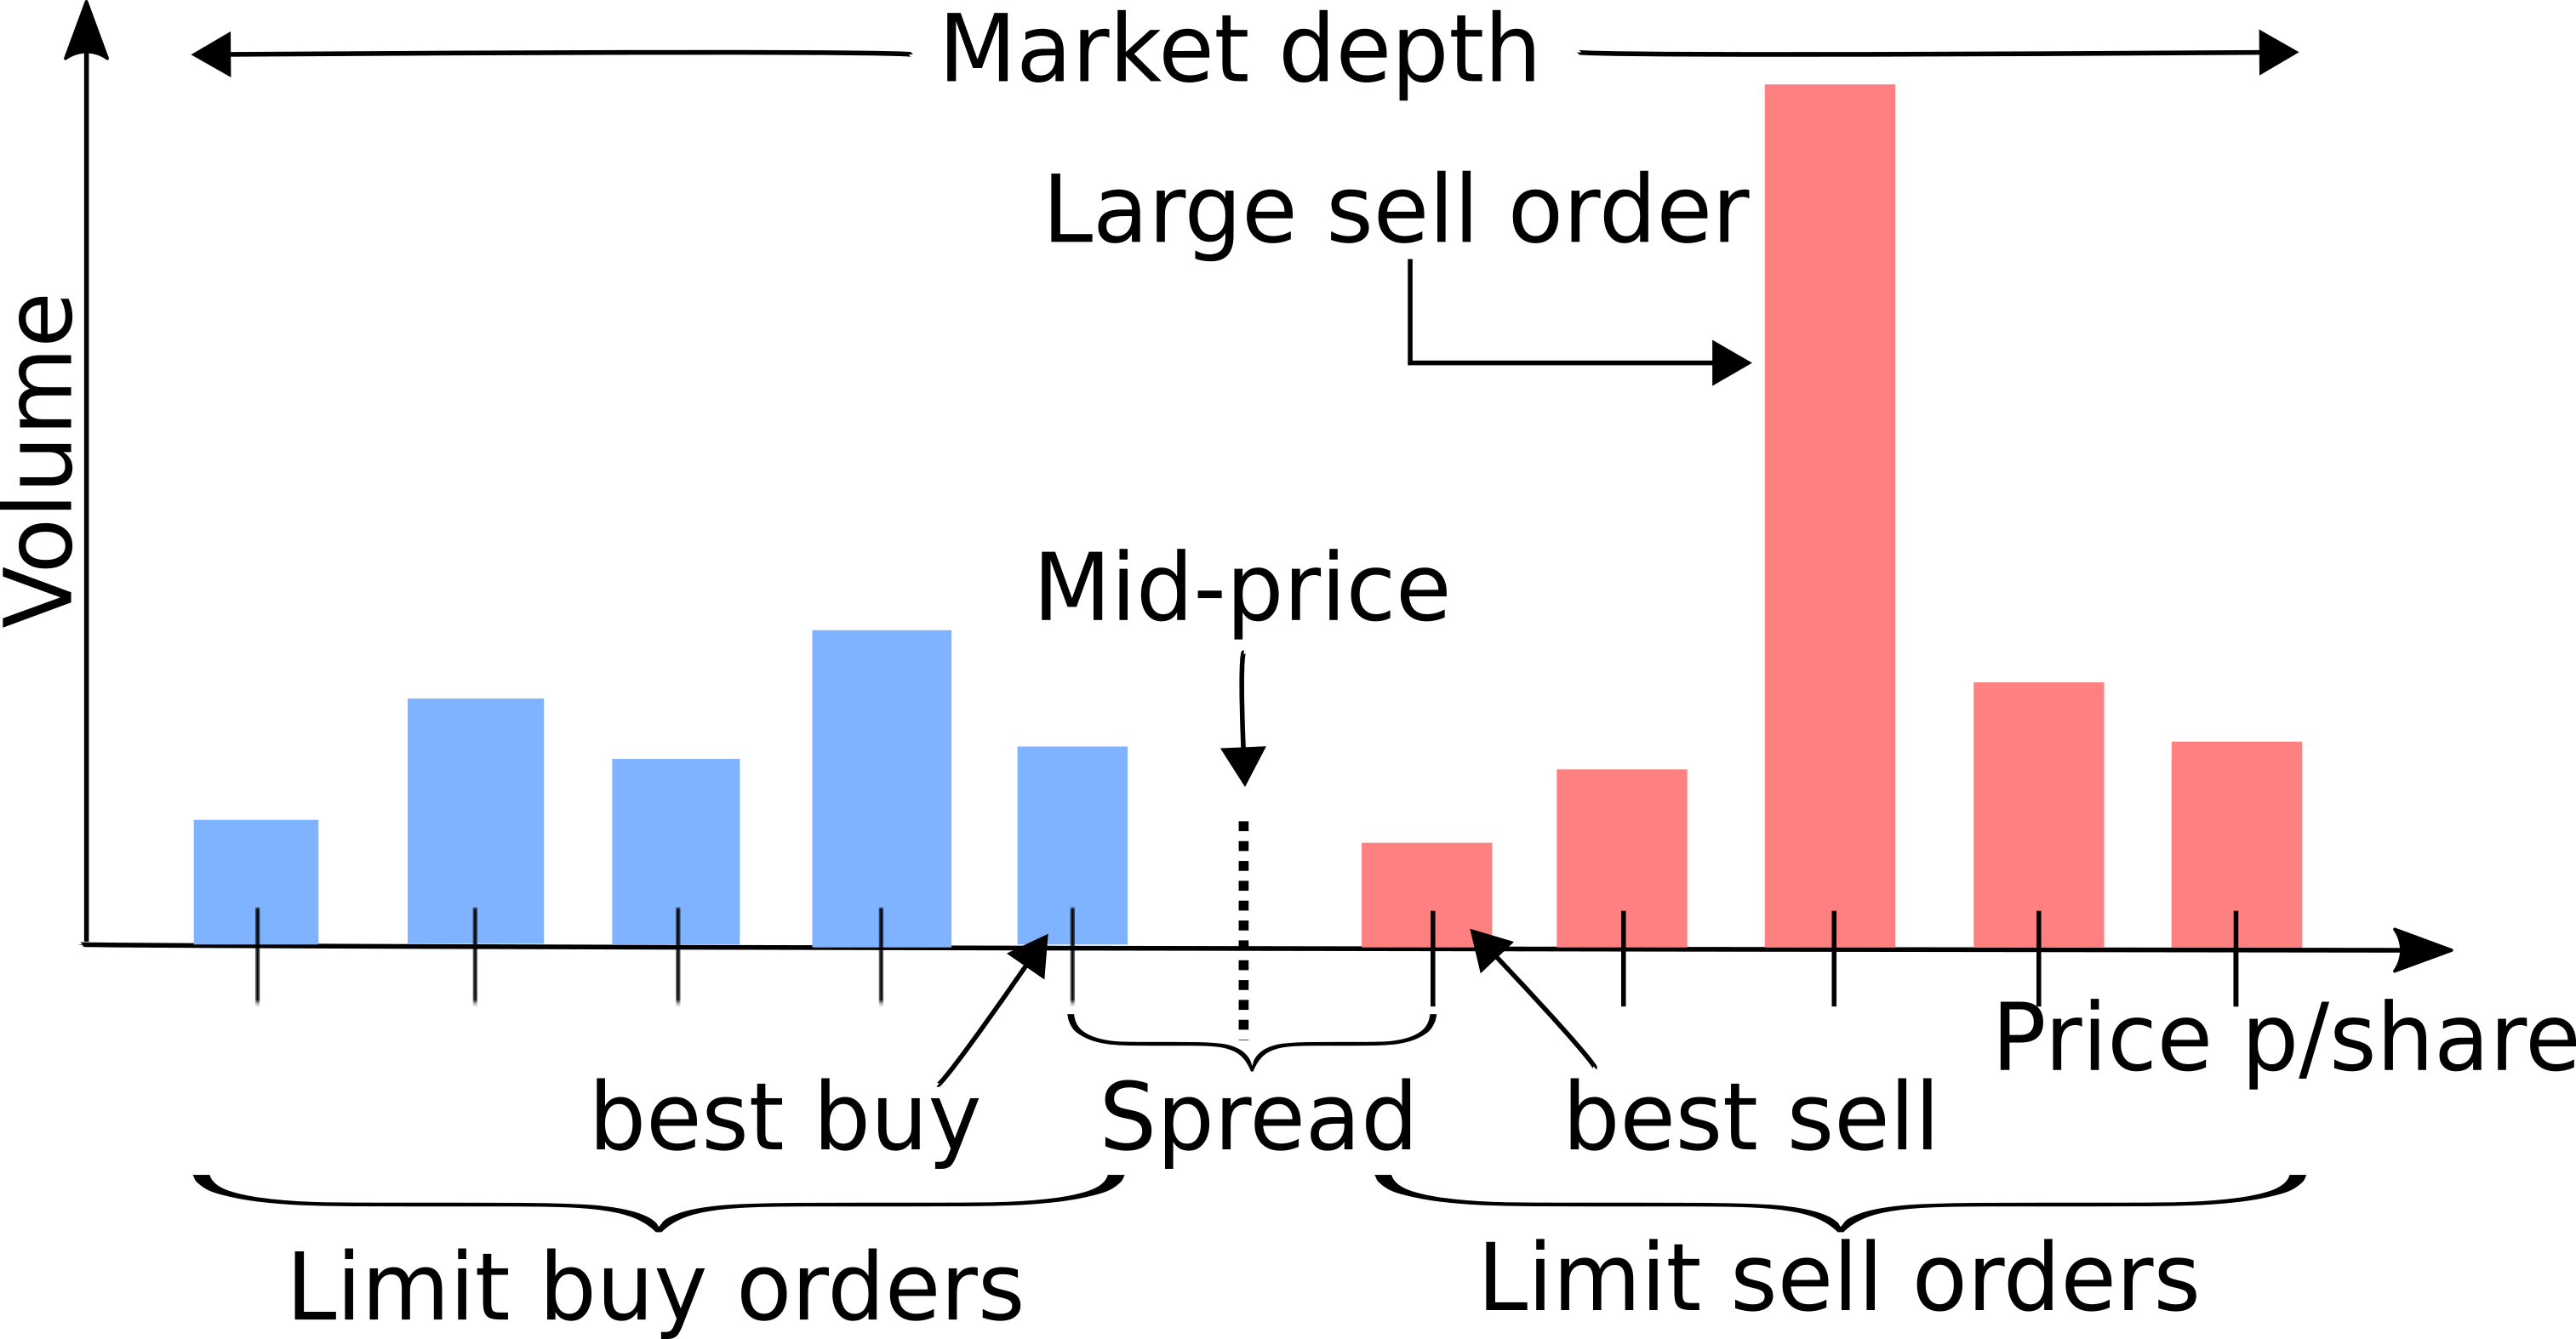
\includegraphics[width=10cm]{lob-simple.png}
    }
    \caption{Figure taken from \cite{miranda}. Simplified limit order book and provides understanding of some characteristics.}
    \label{fig:orderbook-simple}
\end{figure}
\hfill
\\
Figure \ref{fig:orderbook-simple} illustrates a simplified order book, from which we can derived the following definitions:

\begin{description}
    \item[Quote:] the last price at which a security was traded.
    This indicates the most recent price on which a buyer and seller agreed upon.

    \item[Book Level:] specifies the position of an order book entry within the side of an order book state. 
    The number of levels presented depends on the exchange. 
    In general Level 1 data corresponds to the most basic information which includes best bid and ask price and size as well as the last traded price with its size.
    Level 2 provides additional insight into the order book entries as the highest (respectively lowest) five to 15 prices are displayed on each side.
    Level 3 is the highest level of order book entries and includes everything from level 2 plus the ability to enter quotes, execute orders and send information. On traditional stock exchanges, this feature is oftentimes exclusive for market makers. \cite{trading-levels}
    
    \item[Market depth:] corresponds to how deep in the order book buyers and sellers have listed offerings.
    
    \item[Volume:] the term volume can relate to the total volume traded over a given time horizon, or can indicate the sum of amounts of what is currently offered to a certain price.
    
    \item[(Best) Bid:] the term \textit{bid} refers to a price on the buyer side and the best bid represents the highest price for which someone is willing to buy a given asset. 
    The best bid appears as the first order book entry on the buyer side, closest to the spread.
    \item[(Best) Ask:] the term \textit{ask} refers to a price on the seller side and the best ask represents the lowest price for which someone is willing to sell a given asset. 
    The best ask appears as the first order book entry on the seller side, closest to the spread.
    \item[Market Price:] the average price between the best bid and best ask price.
    
    \item[Spread:] the difference between the best bid and best ask.
    
    \item[Liquidity:] in an \textit{order driven market}, liquidity is a synonym for the ease of trading.
    Liquidity provided by parties of the opposing side is what effectively enables one to buy and sell securities.
    
    \item[Market Maker:] provides liquidity to the market by posting limit orders which are not immediately executed.
    In return, the market maker pays less fees than a market taker.
    
    \item[Market Taker:] takes liquidity out of the market by either posting either market orders or limit orders which immediately execute.
\end{description}


\section{Match Engine}
\label{sec:match-engine}

Matching engines are responsible for the process of matching buy and sell orders that are submitted to electronic trading networks, like \textit{NASDAQ} or \textit{NYSE} as examples of traditional stock exchanges; or \textit{Bitfinex}, \textit{Bittrex}, \textit{Coinbase} as examples of crypto-currency exchanges.
Without a local match engine, one would be forced to consult such an exchange and either trade on the live market or get access to a test environment, which can be, if existent, still costly.

This section first give the definiton of a trade and subsequently introduces the mechanics of the match engine which is used in this project and acts as one of the key components.

\subsection{Trade}

In order to understand the purpose of the matching process, which is described in more detail below, we first have to define what a \textit{trade} is.
A trade results when the orders (Eq. \ref{eq:order}) from two parties with opposing order side (Eq. \ref{eq:order-side}) agree on an amount and price to trade their shares.
That is,
\begin{equation}\label{eq:trade}
    Trade=\{ ts, side, type, quantity, price \}
\end{equation}
, where $ts$ is the time-stamp when the participants agreed on the exchange of the products, $side \in OrderSide$, $type \in OrderType$, $quantity \in \mathbb{R^+}$ and $price \in \mathbb{R^+}$.

\subsection{Interface}
\label{sec:match-engine-interface}

This match engine enables the simulation and evaluation of order placement without the need to consult an electronic trading network.
Alongside the order that is sent to the match engine (directly or via an electronic trading network), the user can specify a \textit{time horizon} $H$ indicating how long the order should stay active.
The two most commonly used timing mechanisms are:
\begin{description}
    \item[Good Till Time (GTT): ] The order stays in the order book until a specified amount of time is consumed. \textit{(Some implementations declare the same idea as Good Till Date whereas a date and time is provided which specifies until when the order is valid.)}
    \item[Good-Til-Canceled (GTC): ] The order stays in the order book until the user submits a cancellation.
\end{description}
\hfill
\\
Hence, the match engine exposes an interface that represents a function $match$ which takes any type of an \textit{Order} (Section \ref{sec:orders}) and the time horizon $H$ and returns a sequence of \textit{trade} (Eq. \ref{eq:trade}).
That is,
\begin{equation}
    match : Order \times H \rightarrow Trades
\end{equation}
, whereas $|Trades| \in \mathbb{N}$.
The order is \textit{filled} if the sum of the traded quantity is equal to the amount stated in the submitted order, \textit{partially-filled} if the traded quantity is $> 0$ and \textit{not filled} otherwise.
\\
\\
\textit{The matching process behaves different, depending on the submitted order type, and is explained in the following paragraph.}

\subsection{Rules}

The rules presented below are, compared to match engines used in electronic trading networks, are rather primitive, yet correct within the subset of its capability.
The rules used by the order matching engine are mainly derived and simplified from \cite{match-engine}:
\begin{enumerate}
    \item Limit orders (defined in Section \ref{sec:limit-order}) may be partially filled or not filled at all in case of absence of parties on the opposing side.
    
    \item Market orders (defined in Section \ref{sec:market-order}) will execute immediately when an opposite order exists in the market.
    
    \item Market orders may be partially filled, at different prices, depending on liquidity in the opposing side of the book.
    
    \item Limit orders are attempted to be matched from the given point in time forward, or in case of a Good Till Time (GTT) for as long as specified.
\end{enumerate}


\subsection{Limitations}

Since the match engine used in this project is a rudimentary implementation for the purpose of simulating and analyzing order execution and placement, it features only a subset a conventional match engine used by electronic trading networks.
That said, the following limitations have to be taken into consideration:
\begin{description}
    \item[Participants:] first and foremost, the match engine is used locally where no other participants are interacting during its use.
    In order to be able to approximate the most likely outcome, historical data serves as a simulation of participants acting in the market.
    While this is valuable real world data, unfortunately it does not cover 1) the possibility of hidden participants entering or 2) leaving the market upon placing an order from our side.
    Participants who would enter the market would likely be in our favour as they would act as potential buyers and sellers and therefore provide liquidity.
    Participants who leave the market would introduce a slight disadvantage as there would be less liquidity.
    Since both parties are absent, we consider our implementation as a good approximation without a major advantage or disadvantage.
    
    \item[Ordering]this match engine is restricted to simulate the matching of only one order from one participant at a time.
    Hence, any type of ordered processing of incoming orders (typically solved with a queuing system) is not supported.
    However, this functionality is also not required for our purposes.
    
    \item[Timing inaccuracy:] occurs when submitting an order with a time horizon (see Section \ref{sec:match-engine-interface}).
    The fact that we rely on historical data and the time stamps of the orders submitted from participants in the past is a limitation when submitting an order over a certain period of time (GTT).
    It can occur that at the end of the period the order would have some time $t$ left (e.g. a few seconds) but the next following order book state is nearer to the future than $t$ would allow.
    We therefore have to abort the matching process early.
    
\end{description}



\section{Order execution and placement}
\label{sec:execution-placement}

A trader has a variety of options on how to approach a market and fulfill his duties to buy (respectively sell) shares.
The process to do so involves the following two steps: \textit{order execution} and \textit{order placement}, whereas the latter is the main subject of this thesis.
A specific definition is given below.

\subsection{Definitions}
\label{sec:execution-definition}

Many useful definitions which highlight the difficulties related to the order execution domain were stated by Lim et al. \cite{lim2005optimal} and Guo et al. \cite{guo2013optimal}:
\begin{description}
    \item[Order execution:] concerns about optimally slicing big orders into smaller ones in order to minimize the price impact, that is, on a daily or weekly basis.
    \item[Order placement: ] concerns about optimally placing orders within ten to hundred seconds.
    Placing hereby refers to the setting of the limit level for a limit order as described in Section \ref{sec:limit-order}.
    \item[Impact cost:] moving the price up by executing large buy orders (respectively down for sell orders) at once. 
    By splitting up a big order (e.g. V shares) into smaller pieces and spreading the execution over a time horizon $H$, the impact cost can be lessened.
    \item[Opportunity cost:] arises when the price moves against our favour while splitting a big order into pieces and delaying execution. 
    Therefore the opportunity to execute at a better price.
    \item[Execution strategy:] optimizes trade-off between impact cost and opportunity cost and therefore trying to find best execution.
    
    \item[Placement strategy:] optimizes the trade-off between opportunity cost and paying a premium while proceeding an execution strategy.
    
    \item[Return:] the return of an order execution or placement is the difference between the price before the action was placed and the resulted price paid (respectively received) in order to fill the entire order.
    Literature suggests (\cite{nevmyvaka2006reinforcement}) to use the \textit{volume weighted average price} as the return.
    That is,
    \begin{equation}\label{eq:vwap}
        VWAP=\frac{\sum{v_p*p}}{V}
    \end{equation}
    , whereas $p$ is the price paid for $v_p$ shares and $V$ represents the total volume of shares.
    
\end{description}

\subsection{Relevant factors}

According to \cite{nevmyvaka2006reinforcement}, the factors which have an impact on order execution can be categorized into \textit{private variables} $P$ and \textit{market variables} $M$:
\begin{description}
    \item[Private Variables:] include the \textit{amount of time} $t$ that is remaining in order to execute a given \textit{inventory} $i$ of shares.
    The execution can be of either subject: buy or sell.
    \item[Market Variables:] reflect the condition of the market at the time of the execution.
    The condition of the market is conformed by the infinite constellations of characteristics  within an order book as described in Section \ref{sec:ob-characteristics}.
    
\end{description}


\section{Time series}

According to the efficient market hypothesis\cite{malkiel1989efficient}, a stock market reflects all the information available to the market participants at any give time. 
Given the vast information flow, the natural consequence is that financial markets are best described over time. 
More precisely, the definition of a time series is an ordered sequence of values of a variable at equally spaced time intervals \cite{intro-timeseries}.

The nature of time series data originated the applications generally known as Time Series Analysis and Time Series Forecasting. 
Both of which play an important role throughout this project.

\subsection{Time series analysis}

The analysis of data observed at different points in time leads to problems in statistical modelling and inference. 
More specifically, the correlation of adjacent points in time can restrict the applicability of conventional statistical methods which traditionally depend on the assumption that these adjacent observations are independent and identically distributed. 
A systematic approach by which one attempts to answer the mathematical and statistical questions posed by these time correlations is commonly referred to as time series analysis. 
Therefore, mathematical models are developed with the primary objective to provide plausible descriptions for sample data. \cite{shumway2000time}

\subsubsection{Random variables}

A collection of random variables indexed according to the order they are obtained in time serves as a representation of the time series. For example, a time series with three data points ($x_1$, $x_2$, $x_3$) can be considered as a sequence of the random variables $x_1$, $x_2$ and $x_3$, where the random variable $x_1$ denotes the value of the first time period, the variable $x_2$ denotes the value for the second time period and $x_3$ denotes the value for the third time period. While graphically plotting the values of random variables, it is conventional to display the random variables on the vertical axis with the time scale as abscissa. \cite{shumway2000time}
\\
\\
One such example of a time series analysis, that is often times seen in the context of financial data, is the moving average. 

\begin{equation}
    v_t=\frac{1}{3}(x_{t-1}+x_t+x_{t+1})
\end{equation}

Moving average allows to smoothen the series by averaging the current value and its immediate neighbors in the past and future.


\subsubsection{Stationarity}

Some of the time series behaviours, which will be presented within this body of work, may hint that a sort of regularity exist over time.
We refer the notion of regularity using a concept called stationarity, as introduced in \cite{shumway2000time}.
\\
\\
A \textbf{strictly stationary} time series is one for which the probabilistic behavior of every collection of values
${x_{t_1}, x_{t_2}, ..., x_{t_k}}$
is identical to that of the time shifted set
${x_{t_1+h}, x_{t_2+h}, ..., x_{t_k+h}}$
for all time shifts $h=0,\pm1,\pm2,...$
\\
\\
A \textbf{weakly stationary} time series, $x_t$, is a finite variance process such that

\begin{itemize}
    \item the mean value function $\mu_t$ is constant and does not depend on time $t$, and
    \item the autocovariance function $\gamma(s, t)$, depends on $s$ and $t$ only through their difference $|s-t|$.
\end{itemize}

Whereas $\mu_t$ is defined as

\begin{equation}
    \mu_{t}=\mathbb{E}(x_t)=\int_{-\infty}^{\infty} x f_t(x) dx
\end{equation}

with $f_t$ being the \textit{marginal density function} \cite{shumway2000time}.
And $\gamma(s, t)$ is defined as
\begin{equation}
    \gamma(s, t)=cov(x_s, x_t)=\mathbb{E}[(x_s-\mu_s)(x_t-\mu_t)]
\end{equation}

for all time points $s$ and $t$.
\\
\\
\textit{Henceforth, we will use the term stationary to mean weakly stationary; if a process is stationary in the strict sense, we will use the term strictly stationary.}

\subsubsection{Time series forecasting}

In statistics, prediction is a part of statistical inference. 
Providing a means of the transfer of knowledge about a sample of a population to the whole population, and to other related populations is one description of statistics. 
However, this is not necessarily equivalent to the process of predicting over time. 
This process, instead, is known as forecasting and describes the transfer of information across, often to very specific point in, time \cite{wiki-timeseries}. \\
\\
Hence the problem is defined in \cite{ito1993encyclopedic} as: \textit{forecasting future values $X_(t+h)$ where $h > 0$ of a weakly stationary process ${X_t}$ from the known values $X_s$ where $s \leq t$}. 
The integer $h$ is called lead time or forecasting horizon, whereas $h$ stands for horizon.
\\
\\
Forecasting methods can be classified, according to \cite{chatfield2000time}, into three types:
\begin{description}
    \item[Judgemental forecasts:] produce projections based on intuition, inside knowledge, and any other relevant information.
    \item[Univariate methods:] forecast depends on present or past values of the time series on which the forecast is projected. Augmentation by a function of time is possible.
    \item[Multivariate methods:] forecast depends on one or more additional time series variables or multivariate models.
\end{description}
\hfill
\\
\textit{Over the course of this work, we make use of univariate- and multivariate methods.}

\section{Reinforcement Learning}
\label{sec:reinforcement-learning}

This section first aims to describe what Reinforcement Learning is and highlights its differences to other machine learning paradigms. 
We briefly reason why this particular technique might be an appropriate choice for the task of optimising order placement. 
Then, a basic understanding about Markov Decision Processes is provided, after which we explain the interaction between the Reinforcement Learning components, followed by a description of their properties.

\subsection{End-to-end learning}

Reinforcement Learning is a specific learning approach in the Machine Learning (see Figure \ref{fig:ml-rl}) field and aims to solve problems which involve \textit{sequential decision making}.
Therefore, when a decision made in a system affects the future decisions and eventually its outcome, the aim is to learn the optimal sequence of decisions with reinforcement learning.

\begin{figure}[H]
    \centering
    \makebox[\linewidth]{
        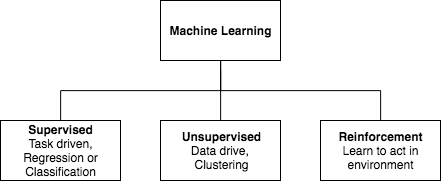
\includegraphics[width=8cm]{ml-rl.png}
    }
    \caption{Categorization of machine learning techniques}
    \label{fig:ml-rl}
\end{figure}
\hfill
\\
In reinforcement learning there is no supervision and instead an agent learns by maximizing rewards.
The feedback retrieved while proceeding a task with a sequence of actions might be delayed over several time steps and hence the agent might spend some time exploring until it finally reaches the goal and can updates its strategy accordingly.
This process can be regarded as \textit{end-to-end learning} and is illustrated in Figure \ref{fig:rl-pipeline}.
\begin{figure}[H]
    \centering
    \makebox[\linewidth]{
        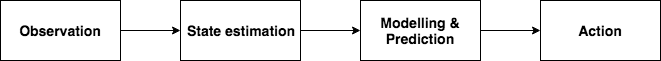
\includegraphics[width=12cm]{rl-pipeline.png}
    }
    \caption{Reinforcement learning end-to-end learning pipeline}
    \label{fig:rl-pipeline}
\end{figure}
The agent makes an \textit{observation} of its environment and estimates a \textit{state} for which it \textit{models and predicts} the \textit{action} to be taken.
Once the action was executed, the agent receives a \textit{reward} and will take this into consideration during during the prediction phases in the future. 
\hfill
\\
\\
In other machine learning paradigms, such as supervised learning, the algorithm learns by presenting a specific situation provided with the right action to do. 
From there, the algorithm tries to generalize the model.
In addition, for reinforcement learning problems, the data is not independent and identically distributed (I.I.D). 
The agent might in fact, while exploring, miss out on some important parts to learn the optimal behaviour. 
Hence, time is crucial as the agent must explore as many parts of the environment to be able to take the appropriate actions. \cite{rl-demystified}

\subsection{Reinforcement Learning in context}
For optimizing order placement in limit order books, statistical approaches have long been the preferred choice.
While statistics emphasizes inference of a process, machine learning on the other hand emphasizes the prediction of the future with respect to some variable.
Although the capabilities of influencing a non-trivial procedure using predictions might be tempting, supervised learning machine learning approaches demand to facilitate complex intermediate steps in order to let the learner interact within the process of buying and selling securities.
Reinforcement learning, as mentioned before, provides the capabilities to model the execution process pipeline whereas the learner improves upon the outcome of the submitted orders. \cite{deeprlcourse}
\\
\\
\textbf{Example:} Since we are working with financial systems, let us assume we want to buy and sell stocks on a stock exchange. 
In reinforcement learning terms, the trader is represented as an \textit{agent} and the exchange is the \textit{environment}.
The details of the environment do not have to be known as it is rather regarded as a black-box.
The agents purpose is to observe the state of the environment: say for example the current price of a stock.
The agent then makes estimates about the situation of the observed state and decides which action to take next – buy or sell. 
The action is then send to the environment which determines whether this was a good or bad choice, for example whether we made a profit or a loss.

\subsection{Markov Decision Process (MDP)}
\label{rl-mdp}

A process such as the one sketched above, can be formalized as a Markov Decision Process.
An MDP is a 5-tuple $<S, A, P, R, \gamma >$ where:
\begin{enumerate}
    \item $S$ is the finite set of possible states $s_t \in S$ at some time step.
    \item $A(s_t)$ is the set of actions available in the state at time step $t$, that is $a_t \in A(s_t)$, whereas $A=\bigcup_{s_t \in S} A(s_t)$
    \item $p(s_{t+1} | s_t, a_t)$ is the state transition model that describes how the environment state changes, depending on the action $a$ and the current state $s_t$.
    \item $p(r_{t+1} | s_t, a_t)$ is the reward model that describes the immediate reward value that the agent receives from the environment after performing an action in the current state $s_t$.
    \item $\gamma \in [0,1]$ is the discount factor which determines the importance of the future rewards.
\end{enumerate}

\subsection{Interaction}

\begin{figure}[H]
    \centering
    \makebox[\linewidth]{
        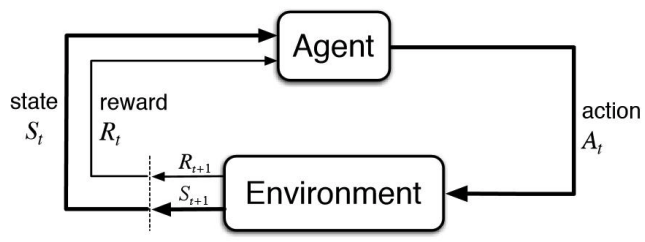
\includegraphics[width=10cm]{rl-overview.png}
    }
    \caption{Figure taken from \cite{rl-demystified}: interaction between a reinforcement learning agent and environment. Illustrating the action taken by the client being in some state which results in some reward and a new state.}
    \label{fit:rl-overview}
\end{figure}
\\
\\
A reinforcement learning problem is commonly defined with the help of two main components: \textit{Environment} and \textit{Agent}.
\\
\\
With the interfaces provided above (Section \ref{rl-mdp}), we can define an interaction process between an agent and environment by assuming discrete time steps: $t=0, 1, 2, ...$

\begin{enumerate}
    \item The agent observes a state $s_t \in S$
    \item and produces an action at time step $t$: $a_t \in A(s_t)$
    \item which leads to a reward $r_{t+1} \in R$ and the next state $s_{t+1}$
\end{enumerate}
\\
\\
During this process, and as the agent aims to maximize its future reward, the agent consults a \textit{policy}, which dictates which action to take given a particular state.

\subsubsection{Policy}

A policy is a function that can be either deterministic or stochastic. 
The distribution $\pi(a|s)$ is used for a stochastic policy and a mapping function $\pi(s) : S \rightarrow A$ is used for a deterministic policy, whereas $S$ is the set of possible states and $A$ is the set of possible actions.
\\
\\
The stochastic \textit{policy} at time step $t$: $\pi_t$ is a mapping from state to action probabilities as a result of the agents experience, and therefore, $\pi_t(s, a)$ is the probability that $a_t=a$ when $s_t=s$.

\subsubsection{Reward}

The goal is that the agent learns how to select actions such that it maximizes its future reward when submitting them to the environment.
We rely on the standard assumption that future rewards are discounted by a factor of $\gamma$ per time-step in the sense that the total discounted reward accounts to $r_1 + \gamma*r_2 + \gamma^2*r_3 + \gamma^3*r_4 + ...)$
\\
Hence we define the future discounted \textit{return} at time $t$ as 

\begin{equation}\label{eq:discounted-return}
R_t=\sum_{i=t}^{T}{\gamma^{i-t}{*}r_{i}}
\end{equation}
, where $T$ is the length of the episode (which can be infinity if there is no maximum length for the episode).
\\
The discounting factor has two obligations: it prevents the total reward from going to infinity (since $0 \leq \gamma \leq 1$), and it allows to control the preference of the agent between immediate rewards and potentially received reward in the future. \cite{rl-demysitifed2}

\subsubsection{Value Functions}

The value of a state $s$ indicates how good or bad a state is for the agent to be in, measured by the expected total reward for an agent starting from this state. Hence we introduce the \textbf{value function}, which depends on the policy the agent chooses its actions from:

\begin{equation}\label{eq:value-function}
V^{\pi}(s)=\mathbb{E}[R_t]=\mathbb{E}[\sum_{i=1}^{T}{\gamma^{i-1}{*}r_{i}}]\ \forall s \in S
\end{equation}
\\
Among all value functions there is an \textbf{optimal value function} which has higher values for all states

\begin{equation}\label{eq:optimal-value-function}
V^{*}(s)=\max_{\pi}V^{\pi}(s)\ \forall s \in S
\end{equation}
\\
Furthermore, the \textbf{optimal policy} $\pi^*$ can be derived as

\begin{equation}\label{eq:value-function-policy}
\pi^{*}=\arg\max_{\pi}V^{\pi}(s)\ \forall{s}\in{S}
\end{equation}
\\
In addition to the value of a state with respect to the expected total reward to be achieved, we might also be interested in a value which determines the value of being an a certain state $s$ and taking a certain action $a$. 
To get there we first introduce the \textbf{Q function}, which takes a state-action pair and returns a real value:

\begin{equation}\label{eq:q-function}
Q:S\times{A}\rightarrow{\mathbb{R}}
\end{equation}
\\
Finally, the \textbf{optimal action-value function} (or \textbf{optimal Q function}) $Q^*(s,a)$ as the maximum expected return achievable after seeing some state $s$ and then taking some action $a$. That is, 

\begin{equation}\label{eq:optimal-action-value-function}
Q^*(s,a)=\max_{\pi}\mathbb{E} [ R_t | s_t=s, a_t=a, \pi ]
\end{equation}

with the policy $\pi$ mapping the states to either actions or distributions over actions. 
\\
\\
The relationship between the \textit{optimal value function} and the \textit{optimal action-value function} is, as already hinted by their names, easily obtained as

\begin{equation}
V^*(s)=\max_{a}Q^*(s,a)\ \forall{s}\in{S}
\end{equation}
\\
and thus the \textit{optimal policy} for state $s$ can be derived by choosing the action $a$ that gives maximum value

\begin{equation}
\pi^*(s)=\arg \max_{a} Q^*(s, a)\ \forall{s}\in{S}
\end{equation}

\subsection{Environment}
\label{sec:rl-environment}

There are two types of environments:
\begin{description}
    \item[Deterministic environment:] implies that both the sate transition model and reward model are deterministic functions. 
    In this setup, if the agent in a given state $s_t$ repeats a given action $a$, the result will always be the same next state $s_{t+1}$ and reward $r_t$.

    \item[Stochastic environment:] implies that there is an uncertainty about the outcome of taking an action $a$ in state $s_t$ as the next state $s_{t+1}$ and received reward $r_t$ might not be the same for each time.
\end{description}
\hfill
\\
\textit{Deterministic environments are, in general, easier to solve as the agent learns to improve the policy without uncertainties in the MDP. }

\subsection{Agent}

The goal of the agent is to solve the MDP by finding the optimal policy, which means finding the sequence of action that lead to maximize the total received reward.
However, there are various approaches to so, which are commonly categorized (see \cite{rl-demysitifed2}) as follows:
\begin{description}
    \item[Value Based Agent:] the agent starts off with a random value function and then finds a new (improved) value function in an iterative process, until reaching the optimal value function. 
    As stated in Eq. \ref{eq:value-function} one can easily derive the optimal policy from the optimal value function. 

    \item[Policy Based Agent:] the agent starts off with a random policy, then finds the value function of that policy and derives a new (improved) policy based on the previous value function, and so on. Each policy is guaranteed to be a strict improvement over the previous one (unless it is already optimal). As stated in Eq. \ref{eq:value-function-policy}, given a policy, one can derive the value function.

    \item[Actor-Critic Agent:] the agent is a combination of a value-based and policy-based agent. Both, the policy and the reward from each state will be stored.

    \item[Model-Based Agent:] the agent attempts to approximate the environment using a model. It then suggests the best possible behaviour.

    \item[Model-Free Agent:] the agent builds a policy just from experience from which it will derive how to behave optimally to get the most possible rewards.
\end{description}

\subsubsection{Value iteration}

This work makes use of the \textit{value based agent} approach which relies on the \textit{action-value function} (Eq. \ref{eq:optimal-action-value-function}) that obeys an important identity known as the \textbf{Bellman equation}. 
\\
\\
The intuition is that: if the optimal value action-value $Q^*(s',a')$ of the state $s'$ at the next time step $t+1$ was known for all possible actions $a'$, the optimal strategy is to select the action $a'$ which maximizes the expected value of $r+\gamma*Q^*(s',a')$,

\begin{equation}\label{eq:bellman}
Q^*(s,a)=\mathbb{E}[r+\gamma \max_{a'} Q^*(s',a')] \ \forall{s}\in{s},  a\in{A}
\end{equation}
\\
The idea behind the many reinforcement learning algorithms which follow the iterative value approach is to estimate the action-value function by using the Bellman equation as an iterative update,
\begin{equation}
Q_{i+1}(s,a)=\mathbb{E}[r+\gamma \max_{a'}Q_{i}(s',a')]
\end{equation}
\\
Value iteration algorithms then converge to the \textit{optimal action-value} function $Q_{i} \rightarrow Q^*$ as $i \rightarrow \infty$. \cite{sutton1998reinforcement}

\subsection{Deep Reinforcement Learning}

From \cite{deeprlcourse} goes: \textit{``Reinforcement learning can be naturally integrated with artificial neural networks to obtain high-quality generalization''}.
The term \textit{generalization} refers to the action-value function (Eq. \ref{eq:optimal-action-value-function}) and the fact that this value is estimated for each state separately--which becomes totally impractical in for large state spaces that can occur in real world scenarios.
A function approximator is therefore a common choice to to estimate the action-value function instead. Typically a linear function approximator is being used but in deep reinforcement learning, one uses a non-linear function approximator; particularly a neural network with weights $\theta$. The \textit{action value function} therefore becomes

\begin{equation}
Q(s, a; \theta) \approx Q^*(s,a)
\end{equation}
\\
In terms of the previously described reinforcement pipeline, the use of a function approximator simplifies this process by replacing state estimation and modelling components by a perception, as shown in Figure \ref{fig:drl-pipeline}:
\begin{figure}[H]
    \centering
    \makebox[\linewidth]{
        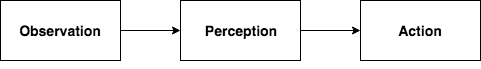
\includegraphics[width=12cm]{drl-pipeline.png}
    }
    \caption{Deep Reinforcement learning end-to-end learning pipeline}
    \label{fig:drl-pipeline}
\end{figure}

\chapter{Related Work}
\label{chap:related-work}

The literature for the order placement problem is, relative to the execution problem, sparse (confirmed by Guo et al. \cite{guo2013optimal}).
In this Chapter we provide an overview of the related work, upon which this project is built on or insight was taken from.
We first give insight into an empirical study about the general behavior of order placements, which serves as a conceptual basis for this project.
Subsequently, a statistical approach is presented to provide contrast to the following overview of previous machine learning approaches.
The latter serve as a guideline on how to model the reinforcement learning process of this thesis.

\section{Execution/Placement behaviour}

Kearns et al. \cite{nevmyvaka2005electronic} determine which limit order price results in the most advantageous execution price.
At first, the \textit{expected execution price} is investigated with respect to the placement of the limit order. 
Based on this analysis the standard deviation of the resulted prices will uncover the \textit{risk} that comes along with limit order placement. 
Finally, by combining the previous two results, an \textit{efficient pricing frontier} can be drawn which highlights the trade-off between risk and returns.

Regarding the definition stated in Section \ref{sec:execution-placement}, their research is in between order execution and placement.
No splitting of orders is being done, however, a time horizon of several hours was chosen, resulting in an evaluation of order placement with an extended time horizon.

\begin{figure}[H]
    \centering
    \makebox[\linewidth]{
        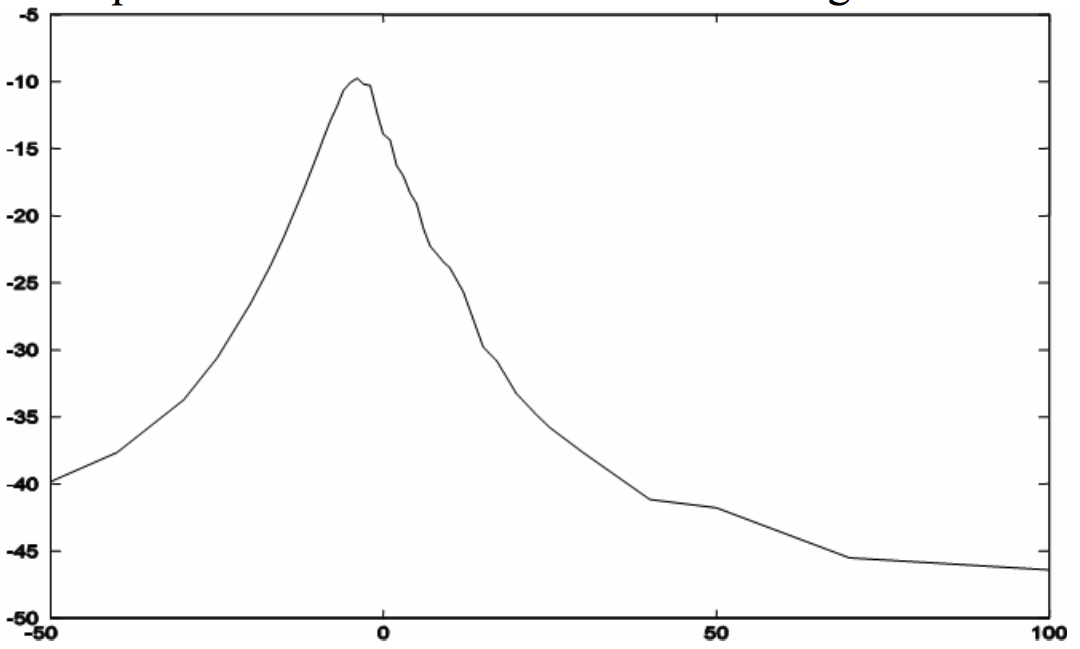
\includegraphics[width=8cm]{kearns-return.png}
    }
    \caption{Taken from \cite{nevmyvaka2005electronic} and illustrates the pricing strategy that produces the most favorable expected execution price.}
    \label{fig:kearns-return}
\end{figure}

Their first approach was to measure the \textit{return} of an execution using the \textit{volume weighted average price} as suggested previously described in Section \ref{sec:execution-definition}.
Figure \ref{fig:kearns-return} shows the return (y-axis) of the expected execution price while acquiring 10,000 shares of MSFT within one hour.
The x-axis represents the limit level reaching from -\$50 to +\$100.
As it is evident from the figure, the most favorable expected execution price occurs when setting the limit price close to the price of the spread, yet on the buyer side with a price approximately \$10 lower than what is currently offered.
The return becomes worse when placing orders more deep in the order book (meaning offering a lower price) as the orders then to not get filled within an hours and instead the inventory has to be bought with a market order at the end of the period.
Likewise, the return can be expected to be lower when placing the order higher in the order book (e.g. deeper in the opposing side of the book, meaning one is willing to pay more).
This is due to the fact that the order is being filled instantly by paying a premium.

\begin{figure}[H]
    \centering
    \makebox[\linewidth]{
        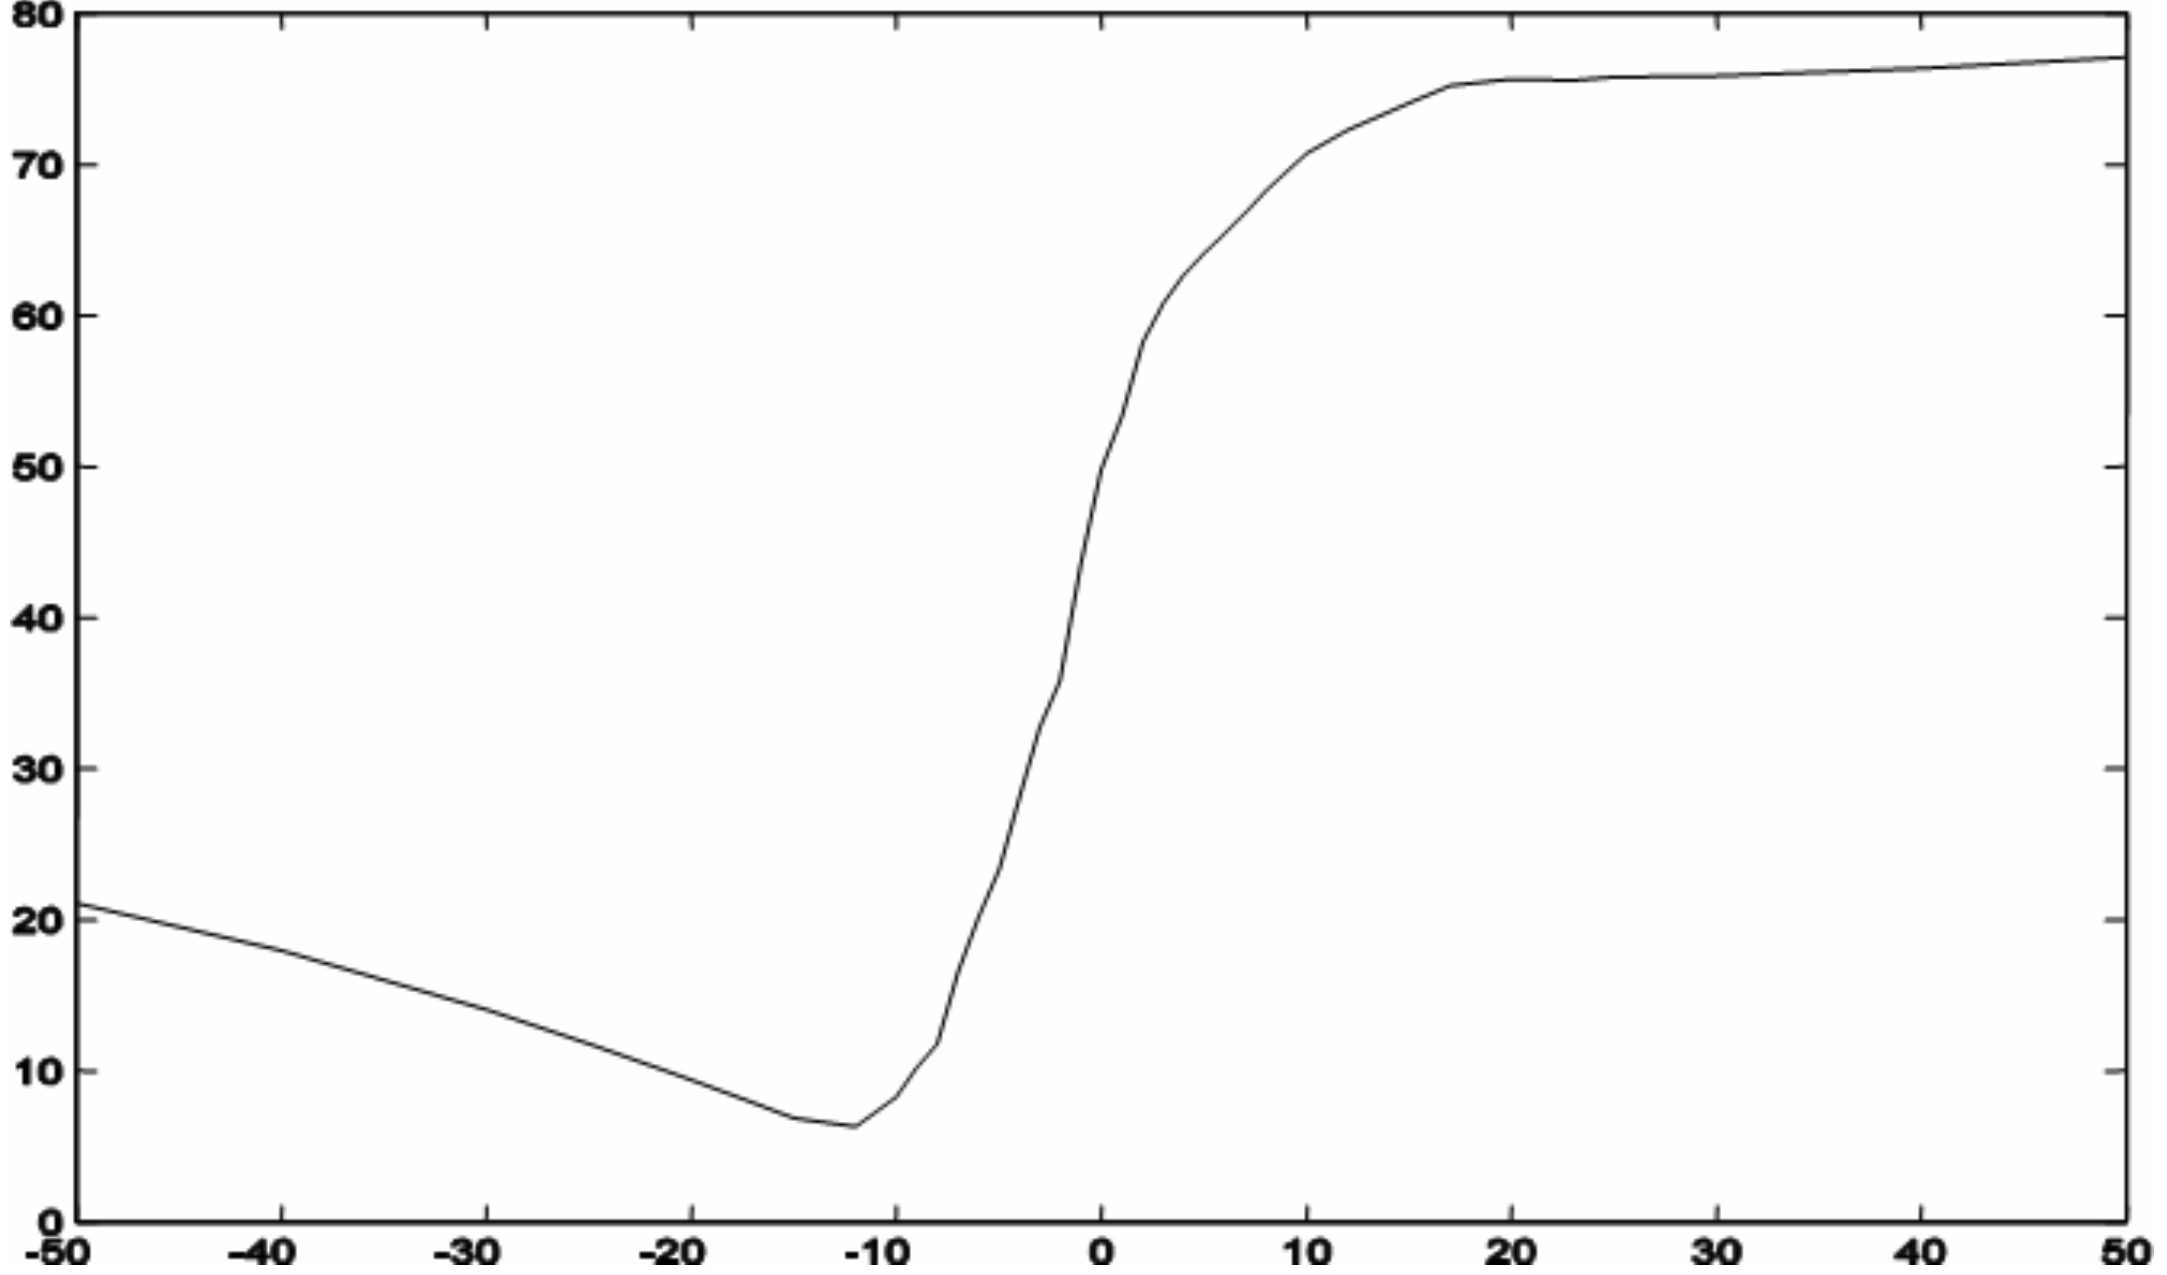
\includegraphics[width=8cm]{kearns-std.png}
    }
    \caption{Taken from \cite{nevmyvaka2005electronic} and illustrates the uncertainty of the expected execution price.}
    \label{fig:kearns-std}
\end{figure}

Risk is being defined as the standard deviation of the returns and is illustrated on the y-axis in Figure \ref{fig:kearns-std}.
Evidently, orders which are placed deep in either of the sides of the book are less likely to be executed and come with a higher uncertainty around the final price.

\begin{figure}[H]
    \centering
    \makebox[\linewidth]{
        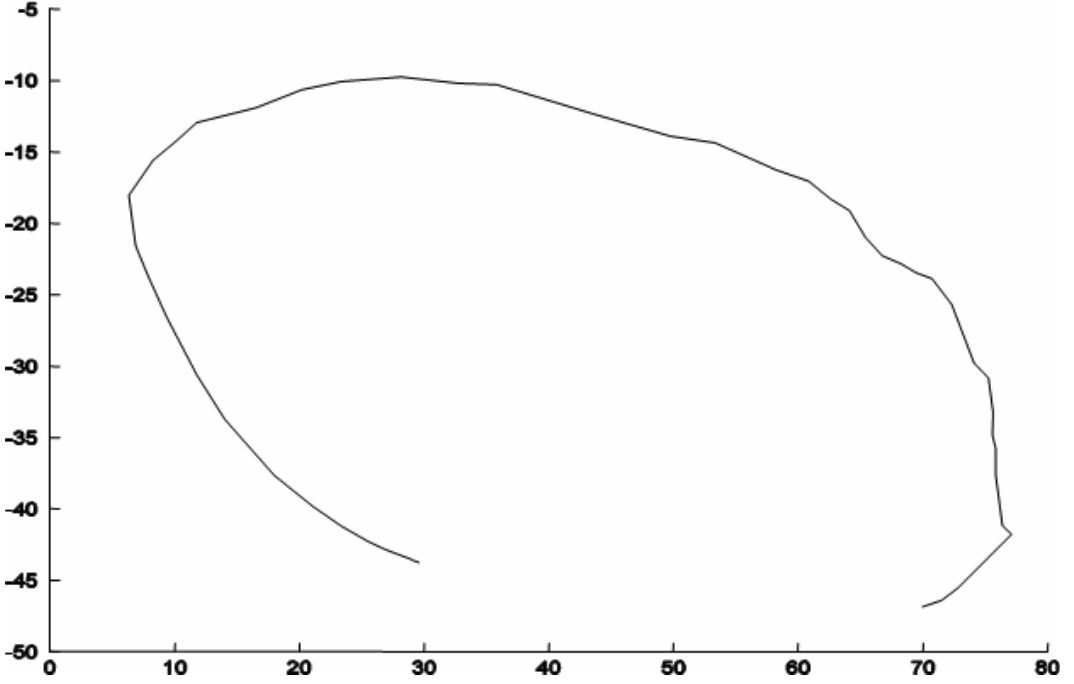
\includegraphics[width=8cm]{kearns-frontier.png}
    }
    \caption{Taken from \cite{nevmyvaka2005electronic} and illustrates the trade-off between risk and return indicated with the efficient pricing frontier.}
    \label{fig:kearns-frontier}
\end{figure}

Lastly, both techniques were combined and result in an efficient pricing frontier (based on the \textit{efficient frontier} initially formulated by Harry Markowitz in 1952 \cite{markowitz1952portfolio}). Therefore, Figure \ref{fig:kearns-frontier} shows the trade-off between the risk (x-axis) and return (y-axis).
In this example, the point of minimum risk is at $(8, 18)$ and the point of maximum returns at $(29, 9)$.
With this technique a trader can decide upon an execution strategy by choosing how much risk and return he is willing to take, and then translate the coordinates back into the corresponding limit level.

\section{Statistical approach}

Profound work in a statistical context has been done by Chaiyakorn Yingsaeree in his dissertation \cite{yingsaeree2012algorithmic}.
A framework is proposed for making order placement decisions based on the trade-off between the profit gained from favorable execution prices and the risk of non-execution.
An execution probability model was developed which estimates the expected payoff (e.g. return) and its variance ($\implies$ risk) while placing orders at a certain limit level, followed by the application of \textit{mean variance optimization} to balance the trade-off.

The framework allows the application of the \textit{liquidity trader problem}, where shares have to be bought using a market order in case the limit order was not filled completely. 
Although this being the main subject of our thesis, we provide an overview of the framework without specific application only, as this would exceed the scope of this overview.
\\
\\
The strategy is to buy $x$ shares in time $T$, whereas the trader is left with the following options:
\begin{enumerate}
    \item Do nothing.
    \item Submit market order at $t=0$ for price $p_{0}^M$
    \item Submit market order at $t=T$ for price $p_{T}^M$
    \item Submit limit order for price $p^L$. If the order is not filled either a market order follows or no action is taken (depending on the use case).
\end{enumerate}
\hfill
\\
A function $U_{E}(p)$ defines the payoff in case of an execution at a price $p$, and a function $U_{NE}(p)$ defines the cost if the order is not executed at the end of the period with market price $p$. 
Consequently, the payoff the trader will receive from submitting a limit buy order at price level $L$ is defined as,
\begin{equation}
    U(p^L) = \begin{cases}
                U_E(p), & \text{if order is executed}.\\
                U_{NE}(p_T^M), & \text{if not executed}.
             \end{cases}
\end{equation}
\hfill
\\
The expected price is compounded of the probability that the limit order at price $p^L$ will be executed before the end of the period together with the distribution of the asset price at the end of the period,
\begin{equation}
    \mathbb{E}[U(p^L)] = P_E(p^L)\ U(p^L) + [1-P_E(p^L)] \int_{-\infty}^{\infty} U_{NE}(p) f_{p_M^T | p^L}(p) dp
\end{equation}
, whereas $P_E(p^L)$ is the probability that the limit order at price $p^L$ will be executed before the end of the period, and $f_{p_M^T | p^L}(.)$ is the probability density function of the asset price at the end of the period. 
\\
Similarly, the variance was drawn as $V[U(p^L)]$ followed by a mean variance optimization step which introduced the utility function,
\begin{equation}
    U_O(p^L) = \mathbb{E}[U(p^L)] - \lambda V[U(p^L)]
\end{equation}
, whereas $\lambda$ serves as a risk factor.
That is, when $\lambda=0$ the trader is concerned about the profit only, and when $\lambda=1$ the trader is equally concerned about profit and risk and missed opportunities.
\\
As a result, the trade-off between profit and risk is defined as,
\begin{equation}
    \hat{p} = \arg\max_{p^L}\ U_O(p^L)
\end{equation}


\section{Machine Learning approaches}
\chapter{Market data curation and feature construction}
\label{chap:data}

In this chapter, we will outline the details of our data collection process, and how this data can subsequently form a historical order book in order to serve as the historical data source for the match engine.
We will describe the way that raw market event data was collected from an exchange (Bittrex\footnote{https://bittrex.com/} in our case) and processed in order to form a historical limit order book.
A sample period from the data set collected will then be investigated in order to find and visualize the properties of the market in question and the behavior of the corresponding market participants.
The goal of the investigation is to find hypotheses which state why certain occurrences might be beneficial to consider for the purpose of limit order placement.
Thus, the findings serve as the basis for the feature construction process which determines the input for the learner.
Therefore, in the last section of this chapter, we will construct features which adequately address the stated hypotheses.
Finally, the features constructed will serve as the observed state that is to be evaluated by the reinforcement learning agents described in Chapter \ref{chap:setup}.

\section{Collection of market events}
\label{sec:data-collection}

In most exchanges in the cryptocurrency domain, real-time market data is freely available. 
There is often a limit as to how far into the past historical data is retained.
However, continuously recording real-time data results in a historical data set which is complete from the time when recording was started and has provided the desired data set for this research.
A historical limit order book consisting of states which store every bid and ask posted by traders is commonly referred to as a \textit{complete order book}.
The process of accumulating the data and building the order book is illustrated in a high level pipeline in Figure \ref{fig:data-pipeline} below.
\begin{figure}[H]
    \centering
    \makebox[\linewidth]{
        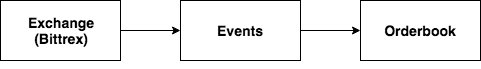
\includegraphics[width=8cm]{data-pipeline.png}
    }
    \caption{Data collection pipeline}
    \label{fig:data-pipeline}
\end{figure}
Therefore, a complete order book is being reconstructed by processing market \textit{events} that have occurred over time with a given ticker (trading pair, in our case USD/BTC).
There are three common types of events, all of which are initiated by a market participant (trader): \textit{order created}, \textit{order cancelled} or \textit{order filled} in the event that a market order crosses the spread, resulting in a trade.

Our exchange of choice for collecting data was Bittrex as this exchange provides a \textit{SignalR}\footnote{https://docs.microsoft.com/en-us/aspnet/signalr/overview/getting-started/introduction-to-signalr} (a library that abstracts \textit{HTTP} and \textit{WebSocket}) interface from which one can extract all status updates (events) from the market.
More specifically, a status update is either a buy or sell order, or a fill (e.g. trade).
Therefore, we subscribed to \texttt{https://socket.bittrex.com/signalr} and filtered the data field \texttt{M} for \texttt{updateExchangeState}.
The data type of the message contains the name of the trading pair and a nonce to identify the unique status update.
That is,
\begin{equation}
    StatusUpdate = \{name, nonce, buy_1,...buy_n, sell_1,...sell_n, fill_1,...fill_n\}
\end{equation}
, whereas $buy \in Order_{Limit}$, $sell \in Order_{Limit}$ (see Eq. \ref{eq:order-limit}) and $fill \in Trade$ (see Eq. \ref{eq:trade}).
In this regard, the orders hold an additional field $type \in \{0,1,2\}$ which specifies whether it was a \textit{create}, \textit{cancel} or \textit{change} in the order, whereby the changes of orders are neglected in our setup as this function is rarely used by traders.

It is evident that multiple events can be sent within one status update message. 
We segmented the status update into separate events with the same nonce, so that each event expressed either a limit order of a side bid or ask or a filled order resulting in a trade.
We then defined an \textit{event} as,
\begin{equation}\label{eq:event-update}
    Event = \{name, nonce, type, isTrade, trade, isBid, order\},
\end{equation}
whereas $isTrade \in \{0,1\}$ and $isBid \in \{0,1\}$ indicating whether the update contains an order or a trade. 
Finally, we made use of the data types defined in Chapter \ref{chap:preliminaries} (Sections \ref{sec:order-book} and \ref{sec:match-engine}) such that $order \in Order_{Limit}$ and $trade \in Trade$.

\section{Reconstruction of an order book with market events}
\label{sec:data-generation}

The next step was to transform the events collected into an order book structure.
By chronologically iterating over the processed events (Eq. \ref{eq:event-update}), we created a new order book state (Eq. \ref{eq:order-book-state}) for each such event.
During this iterative process, we ensured that the correct order book entries remained in future order book states, by handling the events in accordance with their respective type, as follows:
\begin{description}
    \item[Order created:] an order book entry is added to the current state.
    \item[Order cancelled:] the amount of shares as specified in the canceled order is subtracted from the entry in the current state at the corresponding price level.
    \item[Order filled:] the amount of shares traded is subtracted from the entry in the current state at the corresponding price level.
\end{description}
\hfill
\\
As a result, a \textit{list} of order book states is formed which constitutes a historical order book (Eq. \ref{eq:order-book}).
\textit{We acknowledge that a list representation is by no means the highest-performing method of implementing an order book, but for our purposes it is sufficient.}

\vfill

\section{Formulating hypotheses of the market behaviour}
\label{sec:data-hypotheses}

Let us  take a random, \textasciitilde10 minute period of the recorded market event data, and try to extract essential information from either raw events or the order book that has been generated.
Figure \ref{fig:data-price-movement} shows the price movement of the chosen sample period, indicating a movement from \$10,100 to \$10,030 and back within 10 minutes.
We first obtain an insight into the market situation with regard to some of the properties mentioned in Section \ref{sec:ob-characteristics} and understand how market participants place orders.
Our aim is then to find patterns of how market participants behave and how this may affect the market.
Subsequently, we will formulate \textit{hypotheses} which propose why certain properties might be beneficial to the order placement process, and thereby suggest which properties might be worth considering in the feature construction process. 
However, we acknowledge that the observations gleaned are based on a random sample of a historical data set,
By no means does this method guarantees that the same observations are true for any order book.

\begin{figure}[H]
    \centering
    \makebox[\linewidth]{
        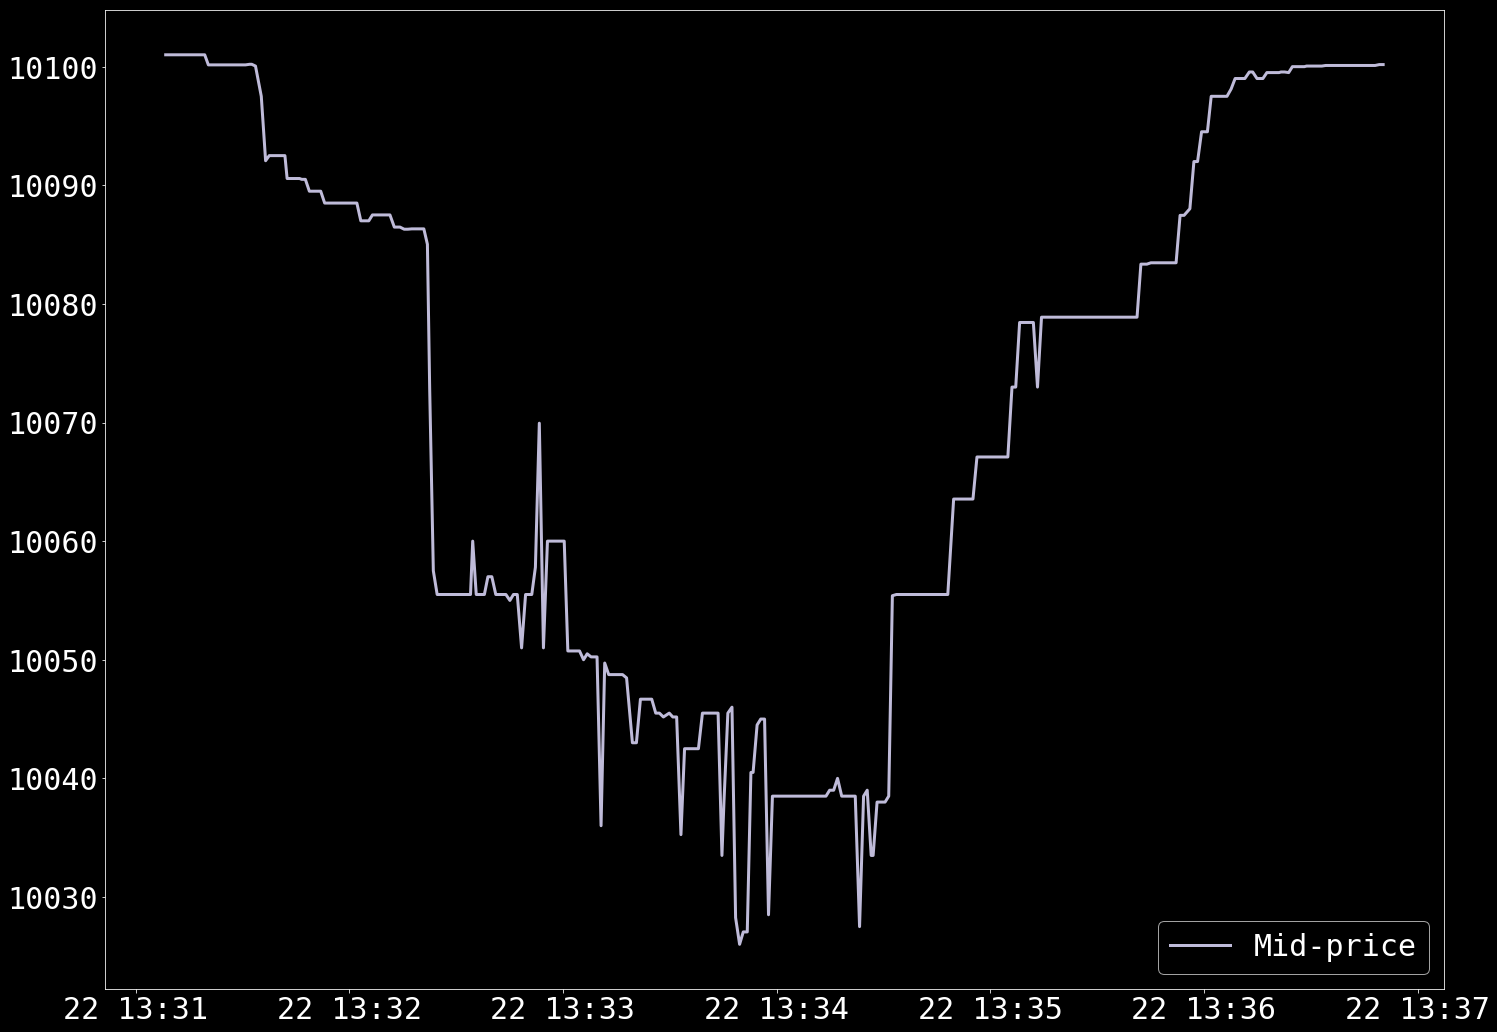
\includegraphics[width=12cm]{ob-price}
    }
    \caption{Price movement of sample data set}
    \label{fig:data-price-movement}
\end{figure}

\subsection{Importance of order prices}
\label{sec:data-hypthesis-order-price}

\begin{figure}[H]
    \centering
    \begin{subfigure}[b]{0.45\textwidth}
        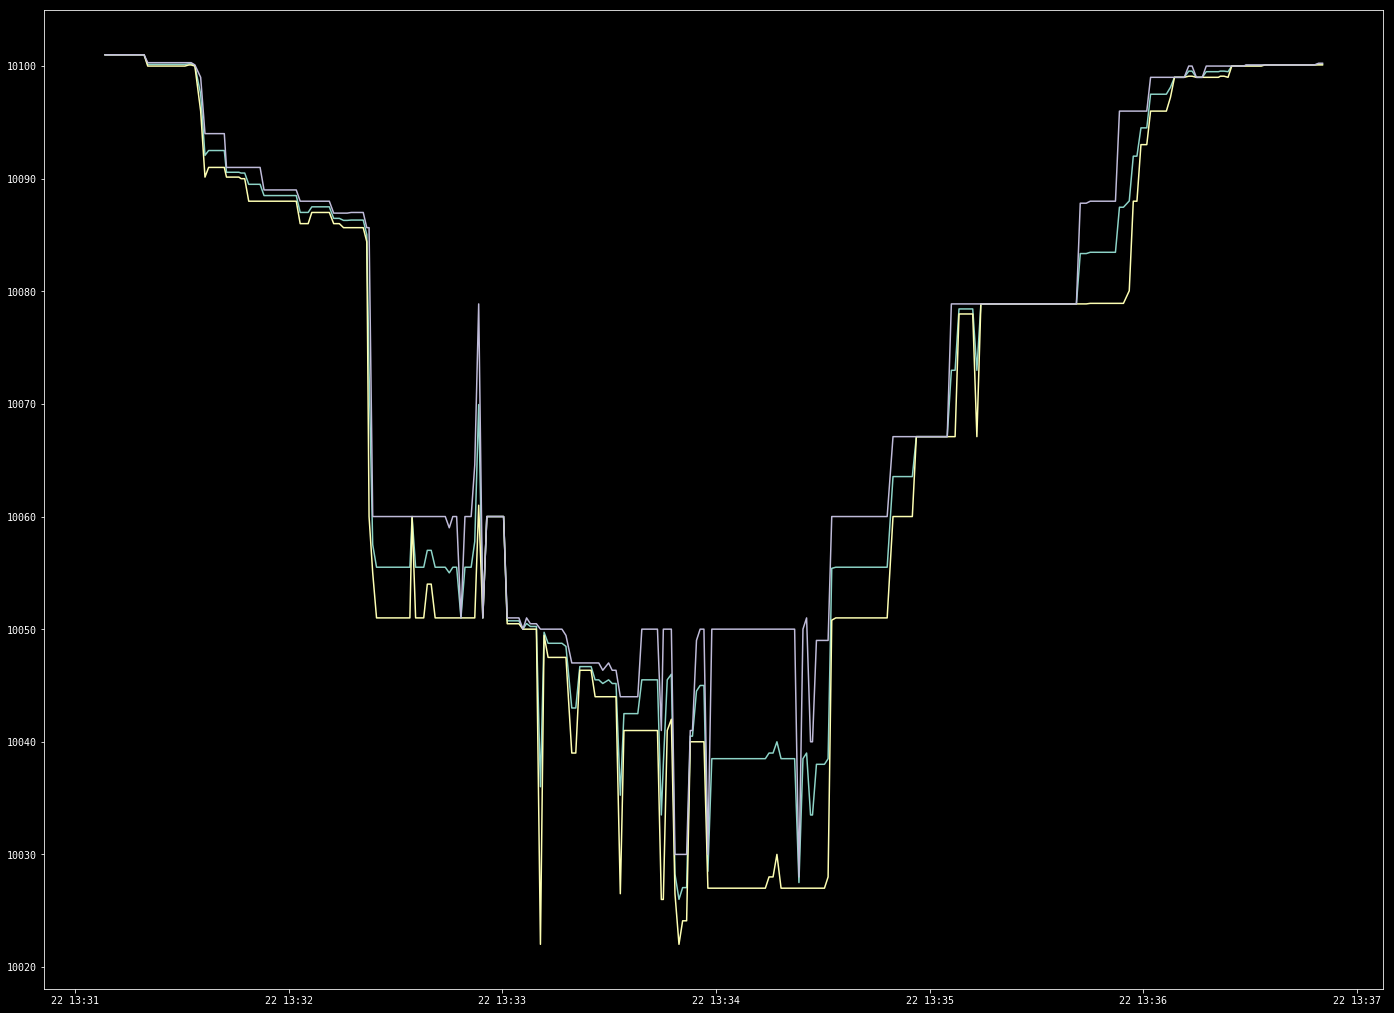
\includegraphics[width=\textwidth]{images/ob-ba-min.png}
        \caption{Best bid and best ask}
        \label{fig:ob-ba-min}
    \end{subfigure}
    ~ %add desired spacing between images, e. g. ~, \quad, \qquad, \hfill etc. 
    %(or a blank line to force the subfigure onto a new line)
    \begin{subfigure}[b]{0.45\textwidth}
        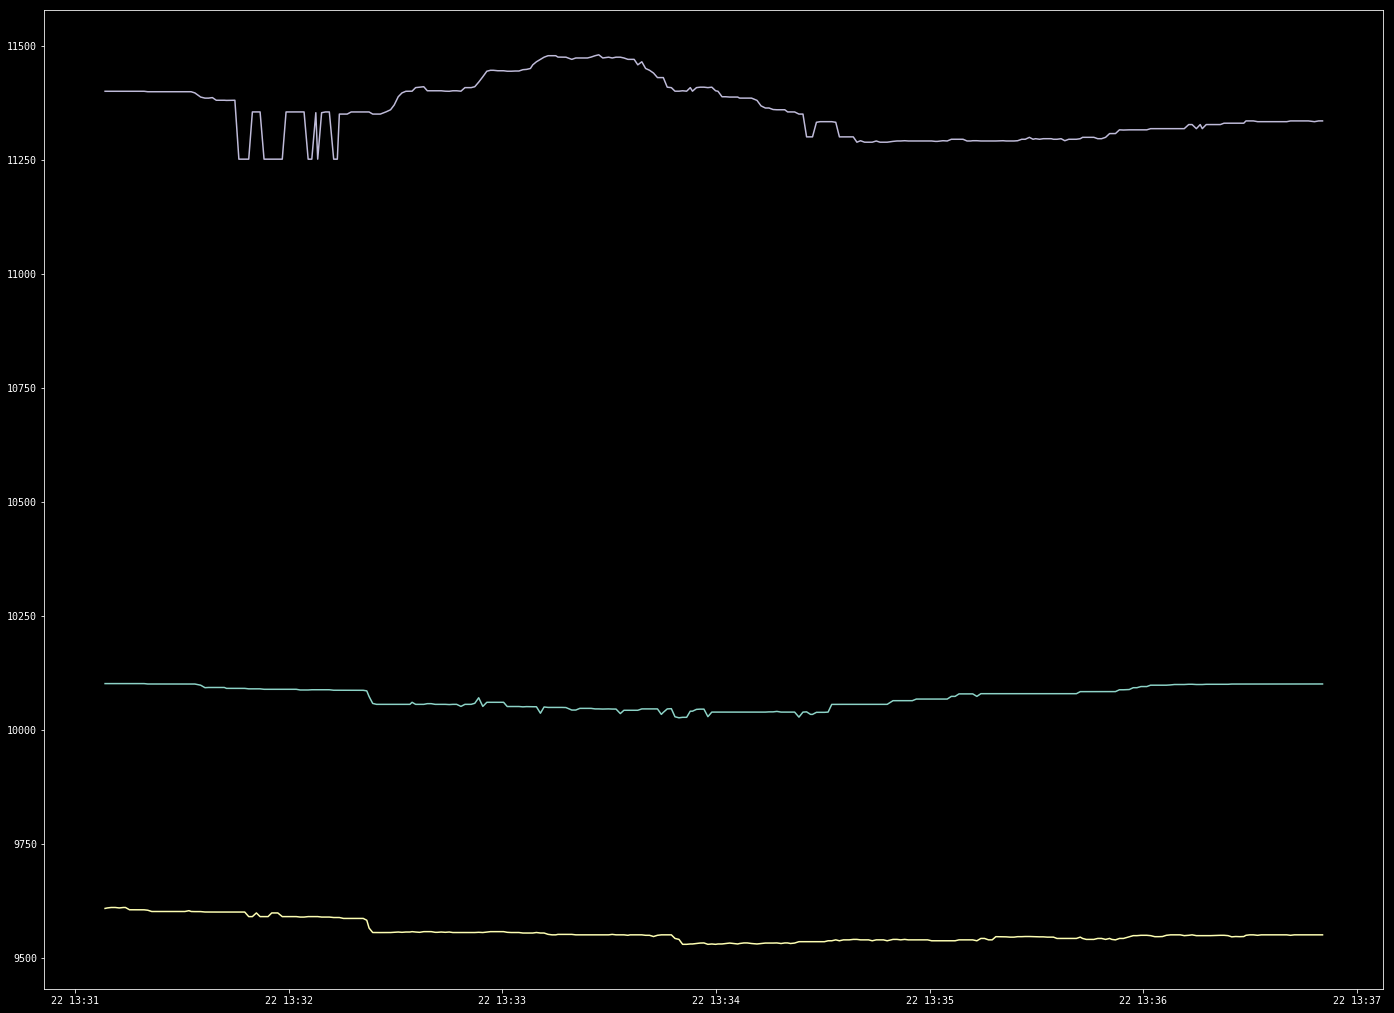
\includegraphics[width=\textwidth]{ob-ba-max}
        \caption{Deepest bid and deepest ask}
        \label{fig:ob-ba-max}
    \end{subfigure}
    \caption{USD/BTC price and bid/ask positions}\label{fig:animals}
\end{figure}

In Figure \ref{fig:ob-ba-min} we show the same price movement including the best bid and ask price.
Furthermore, the deepest level of the bid and ask ask side is shown in Figure \ref{fig:ob-ba-max}.
It is evident that the best bid and ask are close to the market price before and after the price dip, meaning the spread is narrow.
During the dip, the spread widens and is, at times, as large as \$25.
\\
\\
\textit{\textbf{Hypothesis:} participants place limit orders close to the spread when the market price is stable and place them further from the spread when the market price is fluctuating.}
\\
\\
The orders placed at the deepest level on the buyer and seller side undergo a very interesting change.
Immediately before the the price dip, ask prices start to fluctuate as some participants cancel their listings.
On the contrary, bid prices remain much more stable.
Likewise, during the fall and rise of the price, the ask price starts to increase at the deepest level of the seller side. 
This phenomenon is, at first glance, unexpected as one would expect the sell offers to decline as the price falls.
As it can be seen that the price rises shortly after the dip, we can postulate that some sellers' intentions were to incentivize buyers with the fear that sell listings could rise even further
\\
\\
\textit{\textbf{Hypothesis:} sellers incentivize buyers by placing higher prices on limit orders during a price fall.}
%\\
%\begin{figure}[H]
%    \centering
%    \begin{subfigure}[b]{0.45\textwidth}
%        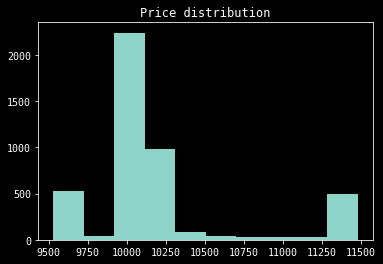
\includegraphics[width=\textwidth]{images/ob-price-bars}
%        \caption{Distribution of prices}
%        \label{fig:ob-price-dist-unfiltered}
%    \end{subfigure}
%    \begin{subfigure}[b]{0.45\textwidth}
%        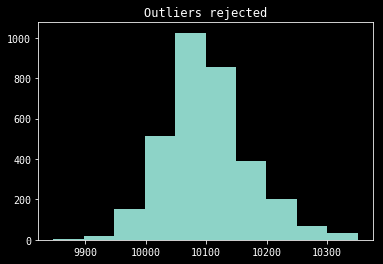
\includegraphics[width=\textwidth]{images/ob-price-bars-rejected}
%        \caption{Distribution of prices (filtered)}
%        \label{fig:ob-price-dist-filtered}
%    \end{subfigure}
%    \caption{Price distribution of events}\label{fig:price-distribution}
%\end{figure}
%
%Figure \ref{fig:ob-price-dist-unfiltered} shows the distribution of prices of all types of events (create, cancel, trade) within this data set.
%As can be seen, most of the events contain prices in the range of the traded price (see Figure \ref{fig:ob-price}) and significantly less below and above this range.
%However, the number of events increase with prices on both, the far end of the buyer and seller side, which supports the above stated hypothesis that orders deep in the book might in fact affect the price movement--even though they were not executed within the spectrum of this data set.
%We then filter events by rejecting outliers of their price $p$ according to standard deviation $\sigma$, $ |p_i - \overline{p}| < m * \sigma_{p} $, whereas $m=2$.
%As a result, Figure \ref{fig:ob-price-dist-filtered} shows the distribution of the prices from the filtered events, that follows a standard distribution.
%The mean lays at approximately \$10'100, the price level before and after the dip.
%\\
%\\
%\textit{\textbf{Hypothesis:} in case of a price dip (or raise) density estimation can be applied to find a more stable price level.}

\subsection{Importance of order volume}
\label{sec:data-hypthesis-order-volume}

It was shown that market participants position orders at different price levels as the asset price moves due to trading.
The second variable in posting orders is the volume and we aim to determine whether or not this is a factor which is affected during price movements in the given sample period.

% \begin{figure}[H]
%     \centering
%     \begin{subfigure}[b]{0.45\textwidth}
%         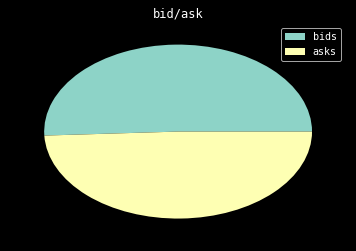
\includegraphics[width=\textwidth]{images/ob-ba-pie-all}
%         \caption{All events}
%         \label{fig:data-imbalance-events}
%     \end{subfigure}
%     \begin{subfigure}[b]{0.45\textwidth}
%         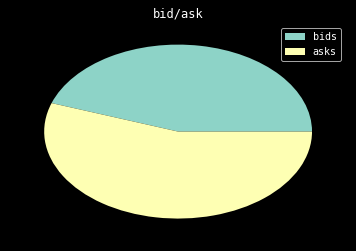
\includegraphics[width=\textwidth]{images/ob-ba-pie-trades}
%         \caption{Trades only}
%         \label{fig:data-imbalance-trades}
%     \end{subfigure}
%     \begin{subfigure}[b]{0.45\textwidth}
%         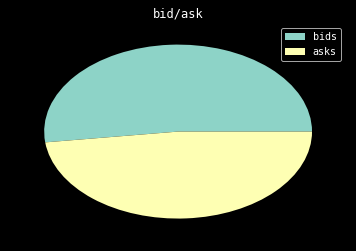
\includegraphics[width=\textwidth]{images/ob-ba-pie-created}
%         \caption{Create order only}
%         \label{fig:data-imbalance-creates}
%     \end{subfigure}
%     \begin{subfigure}[b]{0.45\textwidth}
%         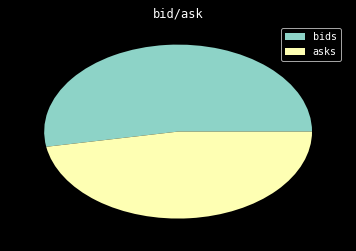
\includegraphics[width=\textwidth]{images/ob-ba-pie-cancelled}
%         \caption{Cancel orders only}
%         \label{fig:data-imbalance-cancels}
%     \end{subfigure}
%     \caption{Bid / Ask volume imbalance}\label{fig:data-imbalance}
% \end{figure}

\begin{table}[H]
\centering
\begin{tabular}{l|l|l|l|l|}
\cline{2-5}
& \textbf{All events} & \textbf{Trades only} & \textbf{Orders created} & \textbf{Orders canceled} \\ \hline
\multicolumn{1}{|l|}{\textbf{Bids}} & 51\%                & 41\%                 & 54\%                    & 57\%                      \\ \hline
\multicolumn{1}{|l|}{\textbf{Asks}} & 49\%                & 59\%                 & 46\%                    & 43\%                      \\ \hline
\end{tabular}
\caption{Bid / Ask volume imbalance}
\label{tbl:data-imbalance}
\end{table}

Table \ref{tbl:data-imbalance} shows the balance between the volumes of bid and ask orders. It does this by categorizing the events as follows: all events, trade events only, order creations, and order cancellations.
It is evident that, even though the price moved significantly within the recorded time range, all the events and trade events only (the first two categories defined above) are well balanced between the bid and ask side.
Further, it is evident that the market participants reacted to the sale of the asset by not only creating but also canceling more buy orders than sell orders.
This indicates that the market participants may have responded to the price dip by canceling their current buy orders and posting them at a lower price in the book.
Interestingly, even though the price rose after the dip, the volumes of creations and cancellations of orders on the seller side were lower.
\\
\\
\textit{\textbf{Hypothesis:} the balance (or imbalance) between volumes of bids and asks of all event types allows us to estimate the future behavior of market participants.}

\subsection{Importance of volume of orders and trades over time}
\label{sec:data-hypthesis-order-trade-volume-time}

So far, volume has been investigated as a sum of events over time.
In order to understand the behavior of participants in greater detail, a \textit{volume map} will provide an insight into single events occurring over time, as shown in the following figures.
The x-axis represents the time stamp and the y-axis is the volume of orders that were placed or resulted in trades.
For visibility reasons, the y-axis follows a log scale, since the volumes of the majority of orders and trades are small and fewer have large volumes.
Participants cannot be assigned to such orders or trades, as the trader "ID" is non-public information.
However, as we will see, one can identify some participants on the basis of their behavior.
Therefore, some of the more obvious patterns are highlighted in the figures.
\begin{figure}[H]
    \centering
    \makebox[\linewidth]{
        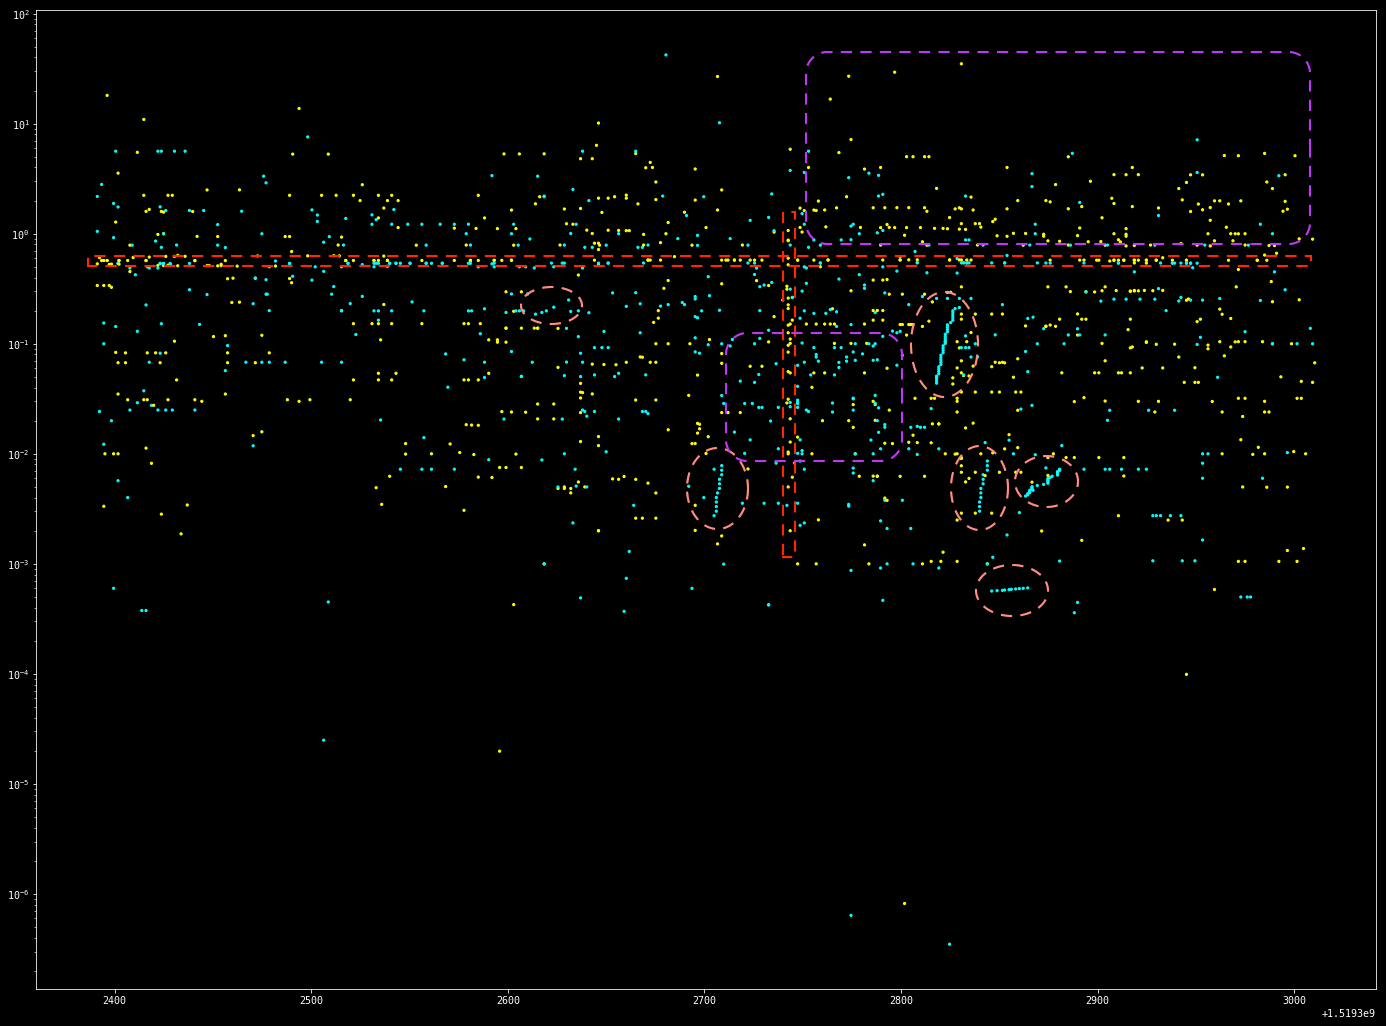
\includegraphics[width=14cm]{images/data-volmap-created}
    }
    \caption{Volume map of created bid and ask orders.}
    \label{fig:data-volmap-crated}
\end{figure}
\ref{fig:data-price-movement}).
\begin{figure}[H]
    \centering
    \makebox[\linewidth]{
        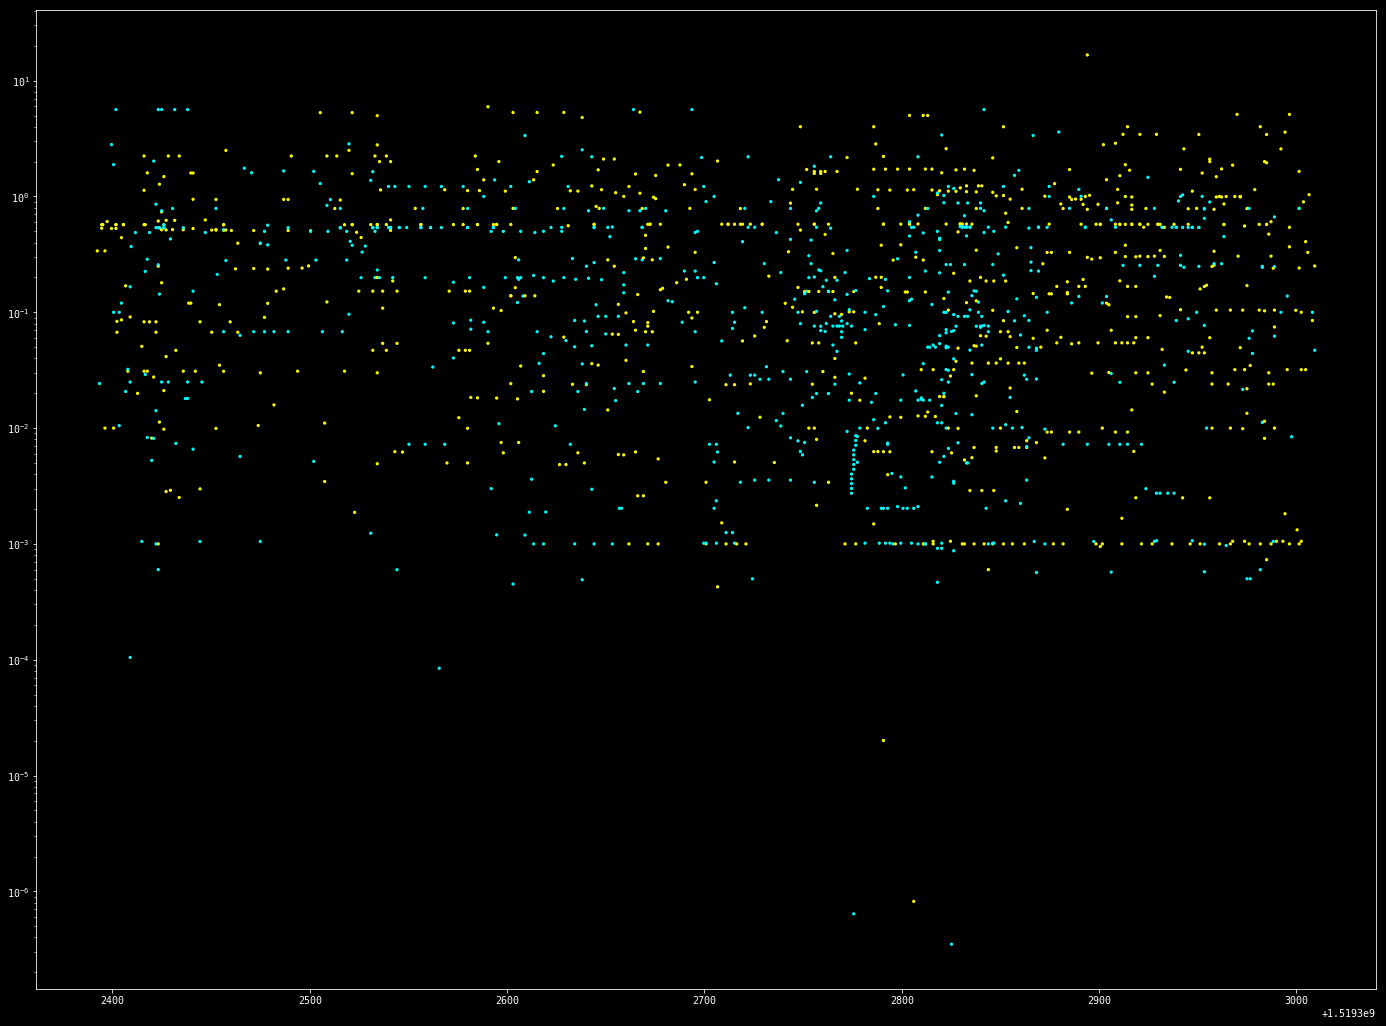
\includegraphics[width=14cm]{images/data-volmap-cancelled}
    }
    \caption{Volume map of cancelled bid and ask orders.}
    \label{fig:data-volmap-cancelled}
\end{figure}
\begin{figure}[H]
    \centering
    \makebox[\linewidth]{
        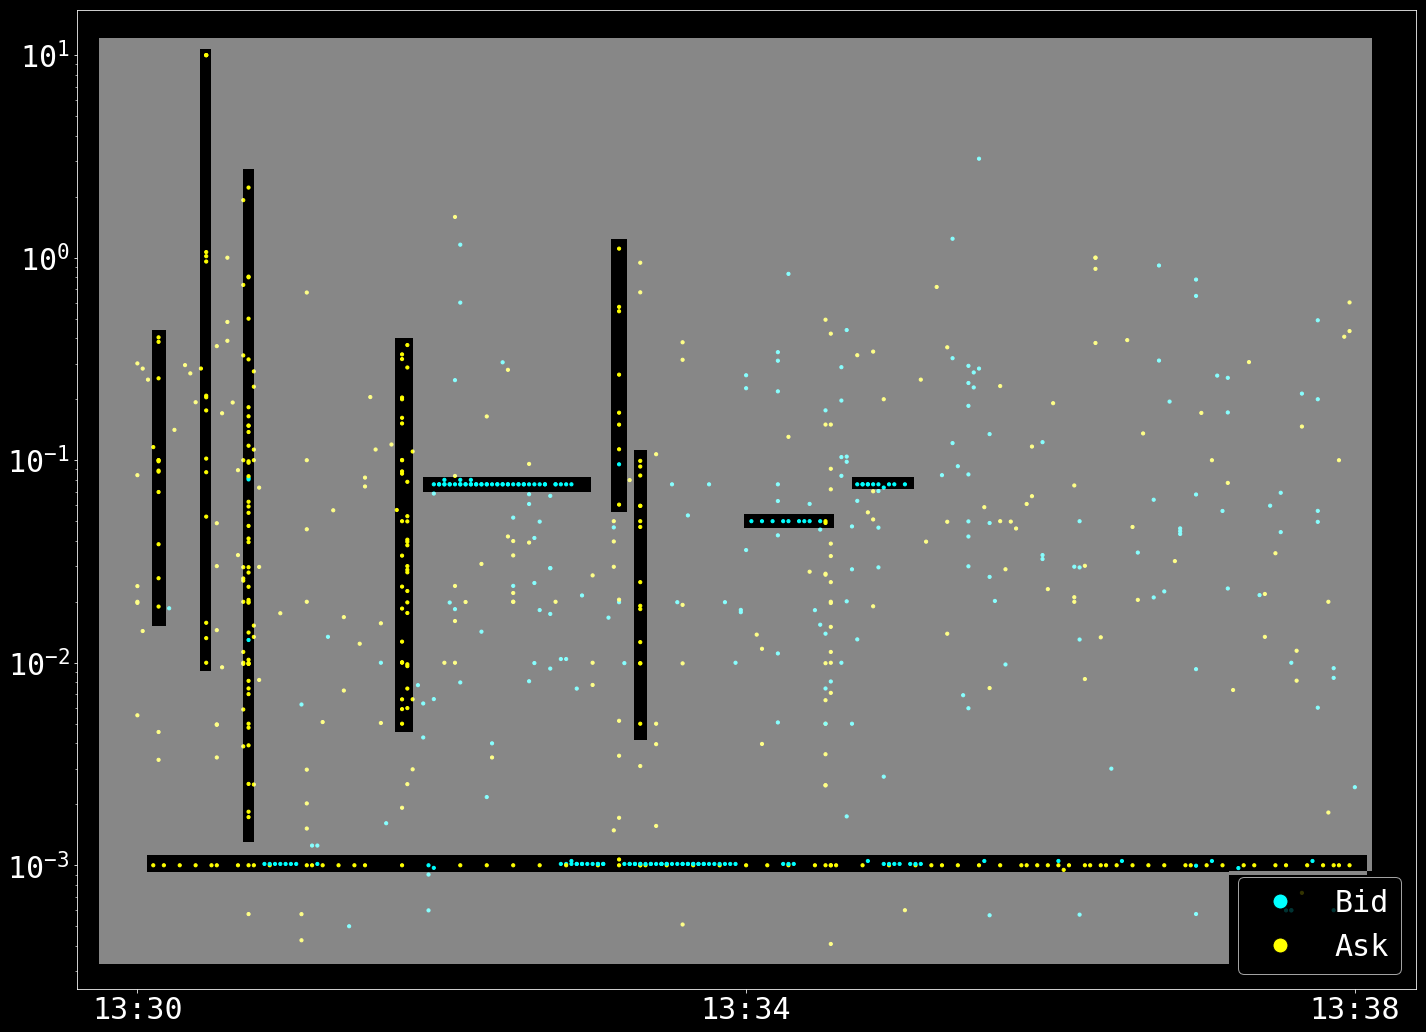
\includegraphics[width=14cm]{images/data-volmap-traded}
    }
    \caption{Volume map of trades initiated by a bid or ask order crossing the spread.}
    \label{fig:data-volmap-traded}
\end{figure}
Figure \ref{fig:data-volmap-crated} shows the volumes of the orders created.
The volumes of most of the orders placed were less than 1.0 BTC and significantly fewer orders had a larger volume, indicating that most of the participants were either willing to buy and sell only small quantities, or split their orders to minimize the market impact.
From a horizontal perspective, one can detect some orders on both sides, bids and asks, that were placed at the same time interval.
This behavior is particularly evident at the regions highlighted on the volume axis just below $10^0$.
This is likely to be one or multiple bots posting orders of the same volume and perhaps at different price levels.
Furthermore, a very distinctive diagonal-shaped pattern occurs when a trader posts orders of varying volumes within a short period of time.
This might be evidence of someone splitting a large order into small pieces (known as a buy- or sell wall).
Surprisingly, this behavior most often appeared both while and immediately after the market price started rising again. To illustrate this, the time stamps from Figure ? can be compared.
\todo[inline]{add reference}

For at least some of the limit orders that did not result in a trade, the cancellation that followed was expected.
Figure \ref{fig:data-volmap-cancelled} shows the canceled orders over time.
Sequences of cancellations emerged more clearly when volumes were just below $10^0$ and at $10^{-3}$, and when these volumes and their respective time intervals correlated with the sequences of the orders created, as shown in ?.
\todo[inline]{refernce}
Hence, it is likely that there was a trader following a strategy which involved creating and canceling orders in equal volumes.
A cancellation of one of the buy-walls that were created is particularly evident in both time stamps shortly after 13:34 and has a volume approximately equal to the one previously discovered during the observation of orders created.
That makes it likely that this wall was created and canceled by a single trader, and perhaps created again as the same pattern occurred again in the order-creation figure at a later time stamp.

So far, only posted limit orders or their cancellations were observed.
Not all of those limit orders might have resulted in a trade. Figure \ref{fig:data-volmap-traded} illustrates the volume map relating to the actual trades that occurred.
It is evident that the volumes of the trades transacted were $10^{-3}$, and oftentimes they had identical time intervals.
Additionally, a rapid series of many consecutive sales occurred around a time that correlates with the fall of the market price.
After the price fell, such sales were not present anymore.
Let us remember that there was one spike during the dip, and the time stamp related to it correlates strongly with the purchases (bids) visible in this figure before 13:34 with volumes of $10^{-1}$.
\\
\\
Various behavioral patterns were observed by investigating events initiated by market participants over time.
For some, their impact on the market price is immediately obvious; for others it is hard to interpret visually.
However, an attempt to find a correlation between the behavior of events and the resulting trades by means of learning techniques seems promising.
\\
\\
\textit{\textbf{Hypothesis:} patterns arising from events in which there were variations in the volumes posted determine future short-term trading behavior which can be exploited in favour of order placement.}

\subsection{Impact of traded price and volume}
\label{sec:data-hypthesis-trade-price-volume}

The price levels and volume of events over time was investigated in respect of each event type in the previous subsections.
Patterns were found and a hypothesis was proposed to the effect that the distribution of volumes of orders is an indicator of the future behavior of market participants. If true, the market price would eventually be influenced and this allows us to determine the optimal order placement.
The next logical step is to investigate the sum of the volumes traded over time, in combination with the price at which the asset was traded.
\begin{figure}[H]
    \centering
    \makebox[\linewidth]{
        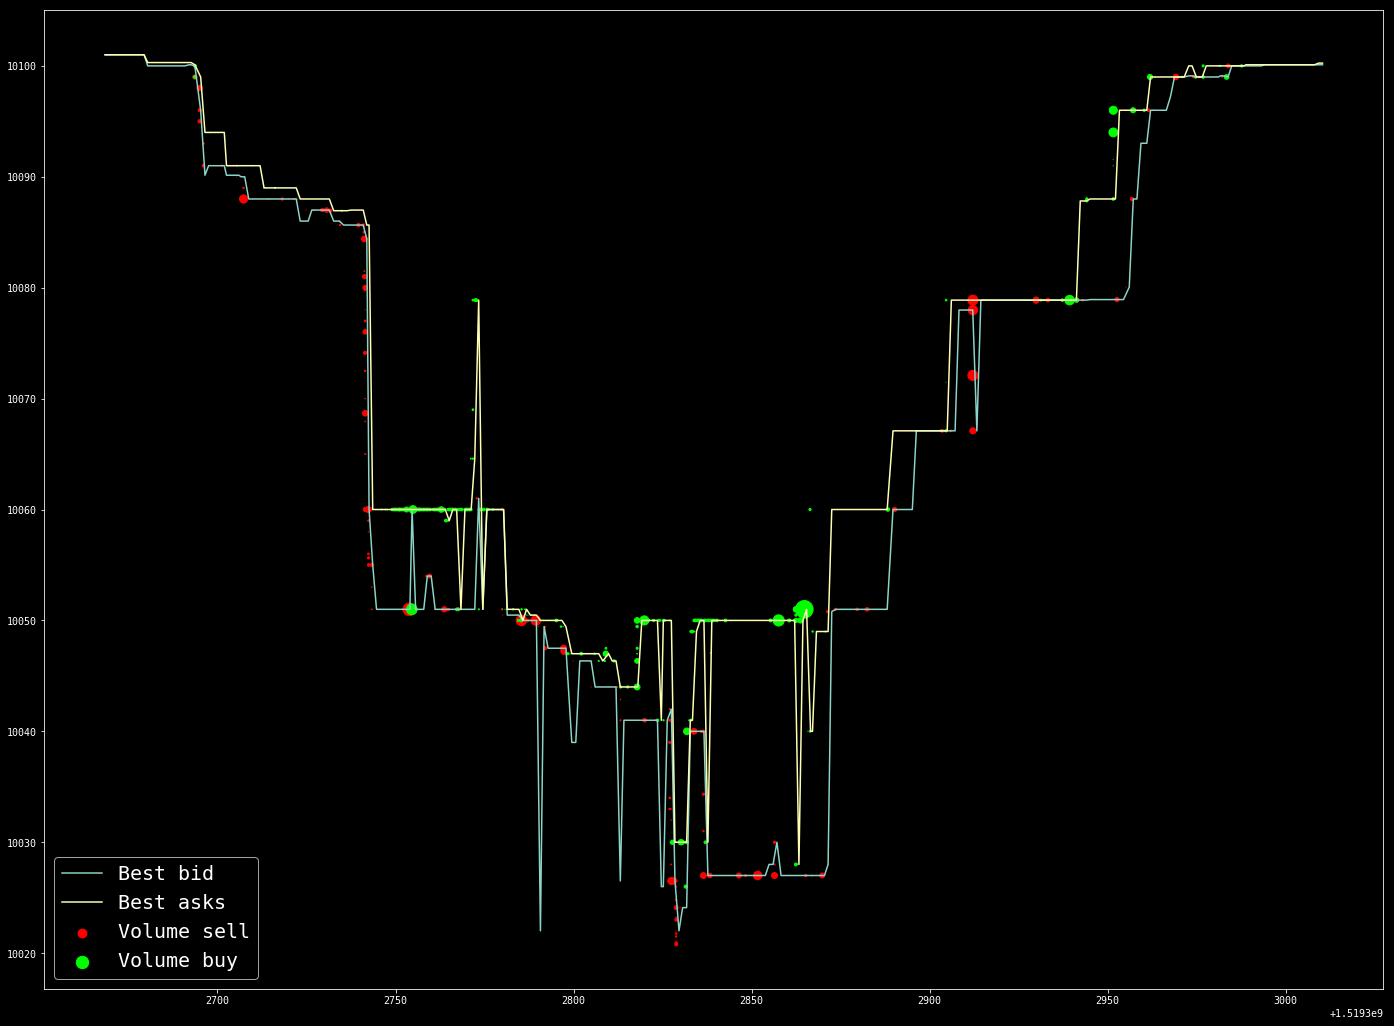
\includegraphics[width=14cm]{data-trade-volume}
    }
    \caption{Relation of trade volume to price movement.}
    \label{fig:data-trade-volume}
\end{figure}
Figure \ref{fig:data-trade-volume} shows the volumes of trades on both bid and ask sides which resulted in a buy or sell at a certain price.
The volumes of these trades are shown as dots of a size that indicates the traded volume and position of each dot defines its respective price.
As is known, a buy appears when one crosses the spread towards the seller side (ask) and a sell appears when crossing towards the buyer side (bid).
One can clearly see how buys are listed at the best ask price and sells are listed at the best bid level.
Before and during the dip, sells appeared consecutively, followed by one large sell transaction.
After that, a series of buy orders with low volumes occurred, and this  caused the minor spike.
Interestingly, a rather large buy trade appeared shortly before the price started to rise again.
Even though sell transactions took place in the middle of the price rise, participants continued buying shortly thereafter.
In conclusion, it is evident that a few trades with small volumes caused a certain noise in the overall trend.
Consecutive trades on one side or a single large trade, however, led the market price to move for a substantially longer period of time in one direction.
\\
\\
\textit{\textbf{Hypothesis:} consecutive small trades or one large trade give an impulse that drives the market price up or down.}


\section{Feature construction}
\label{sec:feature-engineering}
The previous section demonstrated certain trading behaviors of market participants in an order-driven market, which ultimately determines the development of the limit order book. 
Hypotheses were laid out which posit that the outcome in terms of a change in the order book constellation and price development can be related to the aforementioned trading behavior.
This suggests that orders can be placed and filled at limit levels which result in a favorable price.
The following subsections will introduce features that are derived from the previously collected (Section \ref{sec:data-collection}) and processed (Section \ref{sec:data-generation}) data and cover the assumptions stated in Section \ref{sec:data-hypotheses}.
Instead of manually extracting features such as those shown in \cite{nevmyvaka2006reinforcement, hwangdeep, fletcher2010multiple}, the aim of this project is to acquire knowledge directly from raw inputs, similar to a proven, successful method in the gaming sector\cite{mnih2013playing} and which was recently applied in the trading context\cite{lu2017agent}.

\subsection{Feature: price and size of historical orders}
\label{sec:data-feature-1}

The first feature represents the order book (as defined in Eq. \ref{eq:order-book}) and generated in Section \ref{sec:data-generation}.
More precisely, for each sample at time $t$, we use $n$ order book entries (Eq.\ref{eq:order-book-entry}) of $m$ of the order book states (Eq. \ref{eq:order-book-state}) with time stamp $ts \le t$.
As shown in Eq. \ref{eq:feature-bid-ask}, $s_{bidask} \in \mathbb{R^+}^{m\times2\times2n}$ is the state observed by a reinforcement learning agent.
The order book states are ordered such that $m$ is the closest to $t$.
The $n$ order book entries are closest to the spread in which only the price $bp$ (respectively $ap$) and size $bs$ (respectively $as$) are considered.

\begin{equation}\label{eq:feature-bid-ask}
s_{bidask} =\begin{bmatrix}
{\displaystyle \begin{pmatrix}
bp_{11} & bs_{11}\\
bp_{12} & bs_{12}\\
\vdots  & \vdots \\
bp_{1n} & bs_{1n}\\
ap_{11} & as_{11}\\
ap_{12} & as_{12}\\
\vdots  & \vdots \\
ap_{1n} & as_{1n}
\end{pmatrix}} & \begin{pmatrix}
bp_{21} & bs_{21}\\
bp_{22} & bs_{22}\\
\vdots  & \vdots \\
bp_{2n} & bs_{2n}\\
ap_{21} & as_{21}\\
ap_{22} & as_{22}\\
\vdots  & \vdots \\
ap_{2n} & as_{2n}
\end{pmatrix} & \cdots  & \begin{pmatrix}
bp_{m1} & bs_{m1}\\
bp_{m2} & bs_{m2}\\
\vdots  & \vdots \\
bp_{mn} & bs_{mn}\\
ap_{m1} & as_{m1}\\
ap_{m2} & as_{m2}\\
\vdots  & \vdots \\
ap_{mn} & as_{mn}
\end{pmatrix}
\end{bmatrix} \ 
\end{equation}

As the state will be observed by a deep learning agent that makes use of a neural network, the scaling of inputs will contribute to a faster learning process.
We therefore have applied normalization to the prices ($bp, ap$) with respect to the best ask price for each state, that is $ap_{i1}$.
Accordingly, we have also normalized the sizes ($bs, as$) by reference to the size provided at the best ask price $as_{i1}$.
While this method does not scale the values of prices and sizes within a predefined range, the values sill decrease significantly.
Furthermore, empirical observations show that the minimum and maximum prices within a single order book state do not differ by more than ~2\%, which determines the approximate scaling boundary.
\\
\\
This feature incorporates some of the previously stated hypotheses and therefore enables the learner to determine whether the statements are valid or not.
In particular, the feature includes historical order prices (hypothesis \ref{sec:data-hypthesis-order-price}), their volume (hypothesis \ref{sec:data-hypthesis-order-volume} and partly \ref{sec:data-hypthesis-order-trade-volume-time}).
\\
\\
\todo[inline]{Might be unnecessary according to our talk.}
There remain the questions of how large the window of $m$ order books states should be and the number of limit levels that $n$ should be chosen.
The following observation provides an insight into the parameters; however, by no means does it aim to make an estimate of how well the agent may perform under the consideration of a certain parameter setup.

In order to determine the impact of $n$ limit levels, we take the average of 100 evaluations whereas we take 1,000 random order book states for which we measure the Shannon entropy\cite{shannon2001mathematical} for a range of 40 limit levels (maximum of what goes from collection) on the bid and ask side, applied to price and size.
The entropy therefore serves as an indicator of how much information can be gained in respect of each limit level, derived from the change in price and size for each state.

\begin{figure}[H]
    \centering
    \begin{subfigure}[b]{0.45\textwidth}
        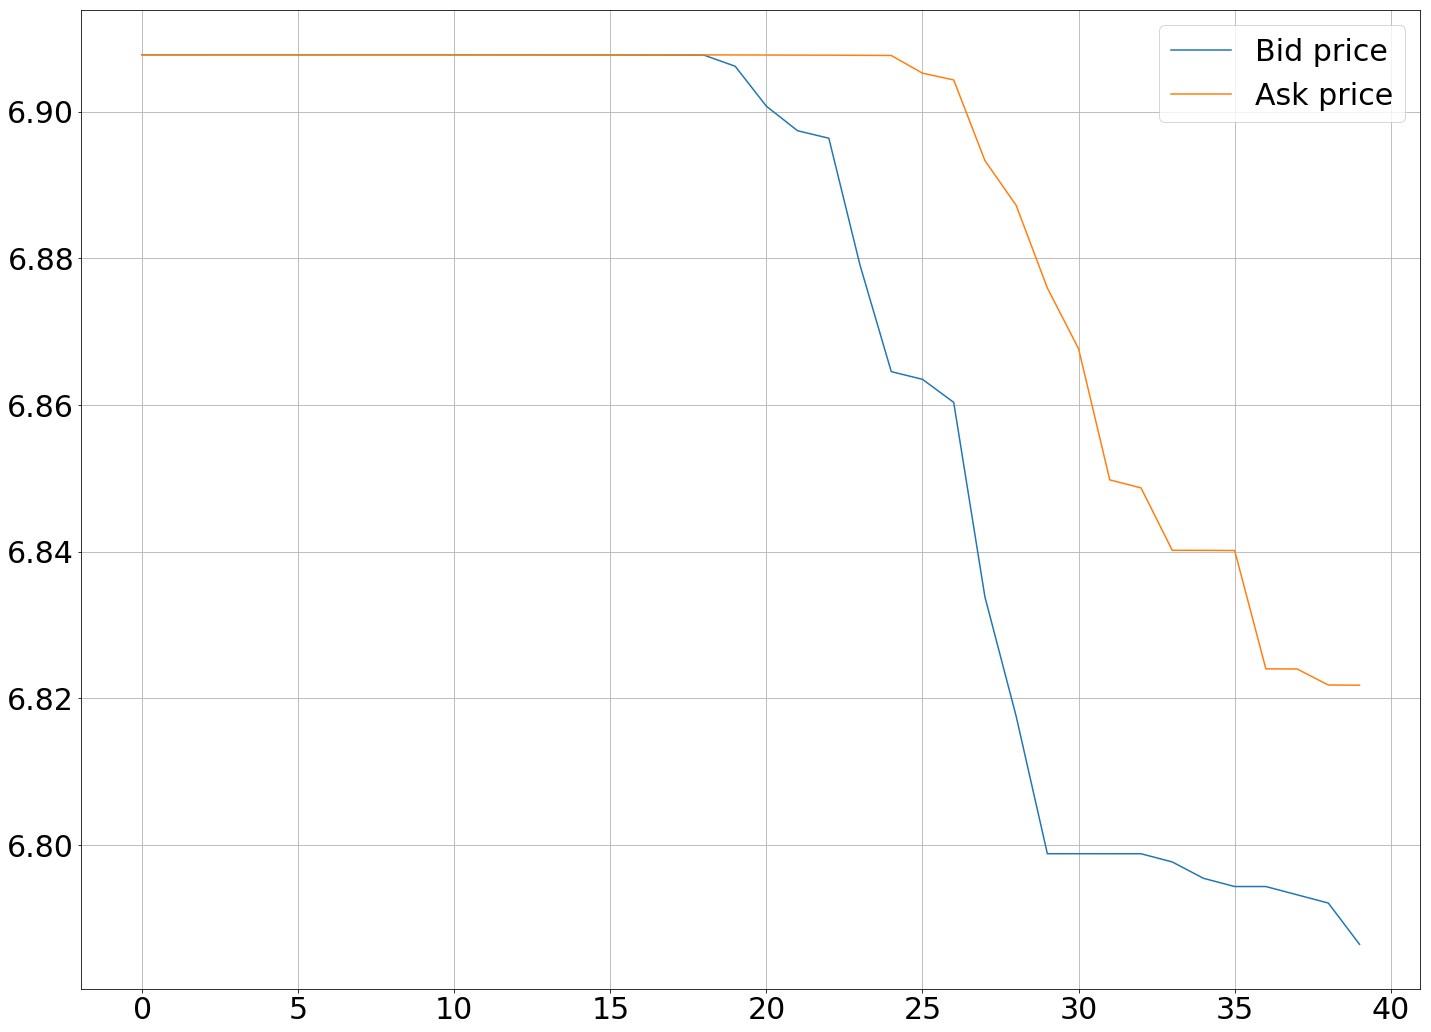
\includegraphics[width=\textwidth]{bidask-price-entropy}
        \caption{Entropy of order prices}
        \label{fig:bidask-price-entropy}
    \end{subfigure}
    \begin{subfigure}[b]{0.45\textwidth}
        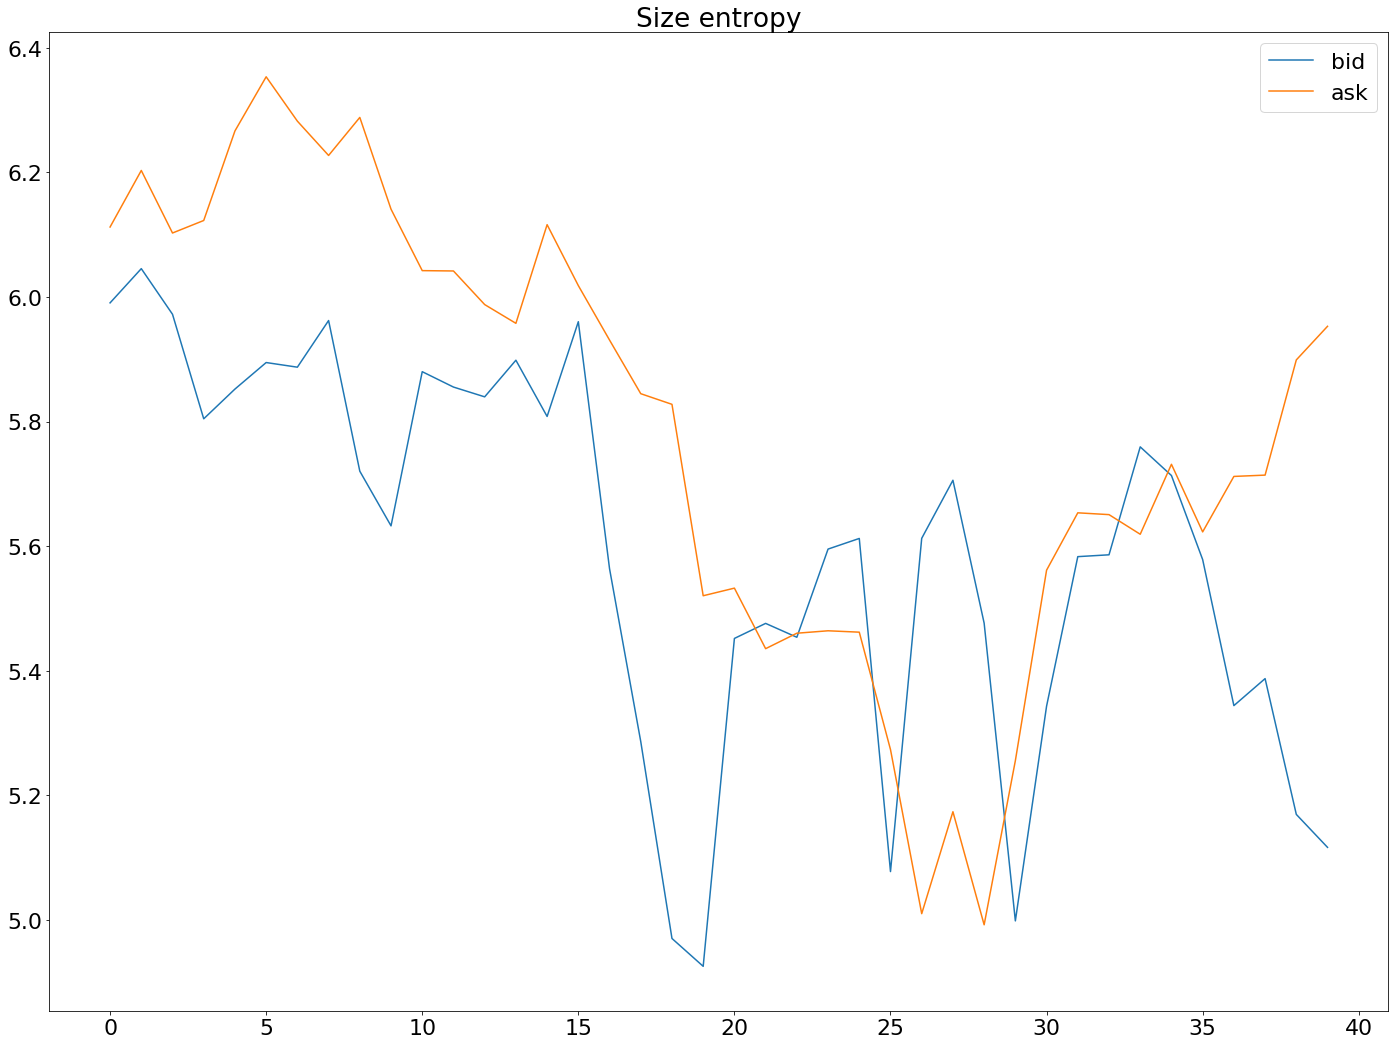
\includegraphics[width=\textwidth]{bidask-size-entropy}
        \caption{Entropy of order sizes}
        \label{fig:bidask-size-entropy}
    \end{subfigure}
    \caption{Entropy measured for 40 limit levels}\label{fig:bidask-entropy}
\end{figure}

It is noticeable that the entropy of prices of limit levels 0-30 on both bid and ask sides remains high, as shown in Figure \ref{fig:bidask-price-entropy}. 
The price becomes slightly more constant for limit levels $>30$. 
The entropy for order sizes, as shown in Figure \ref{fig:bidask-size-entropy}, drops after 20 limit levels, which indicates that the accumulated order size deep in the book is more constant. 
We therefore suggest considering at least 30 limit levels of the bid-ask feature.

\begin{figure}[H]
    \centering
    \begin{subfigure}[b]{0.45\textwidth}
        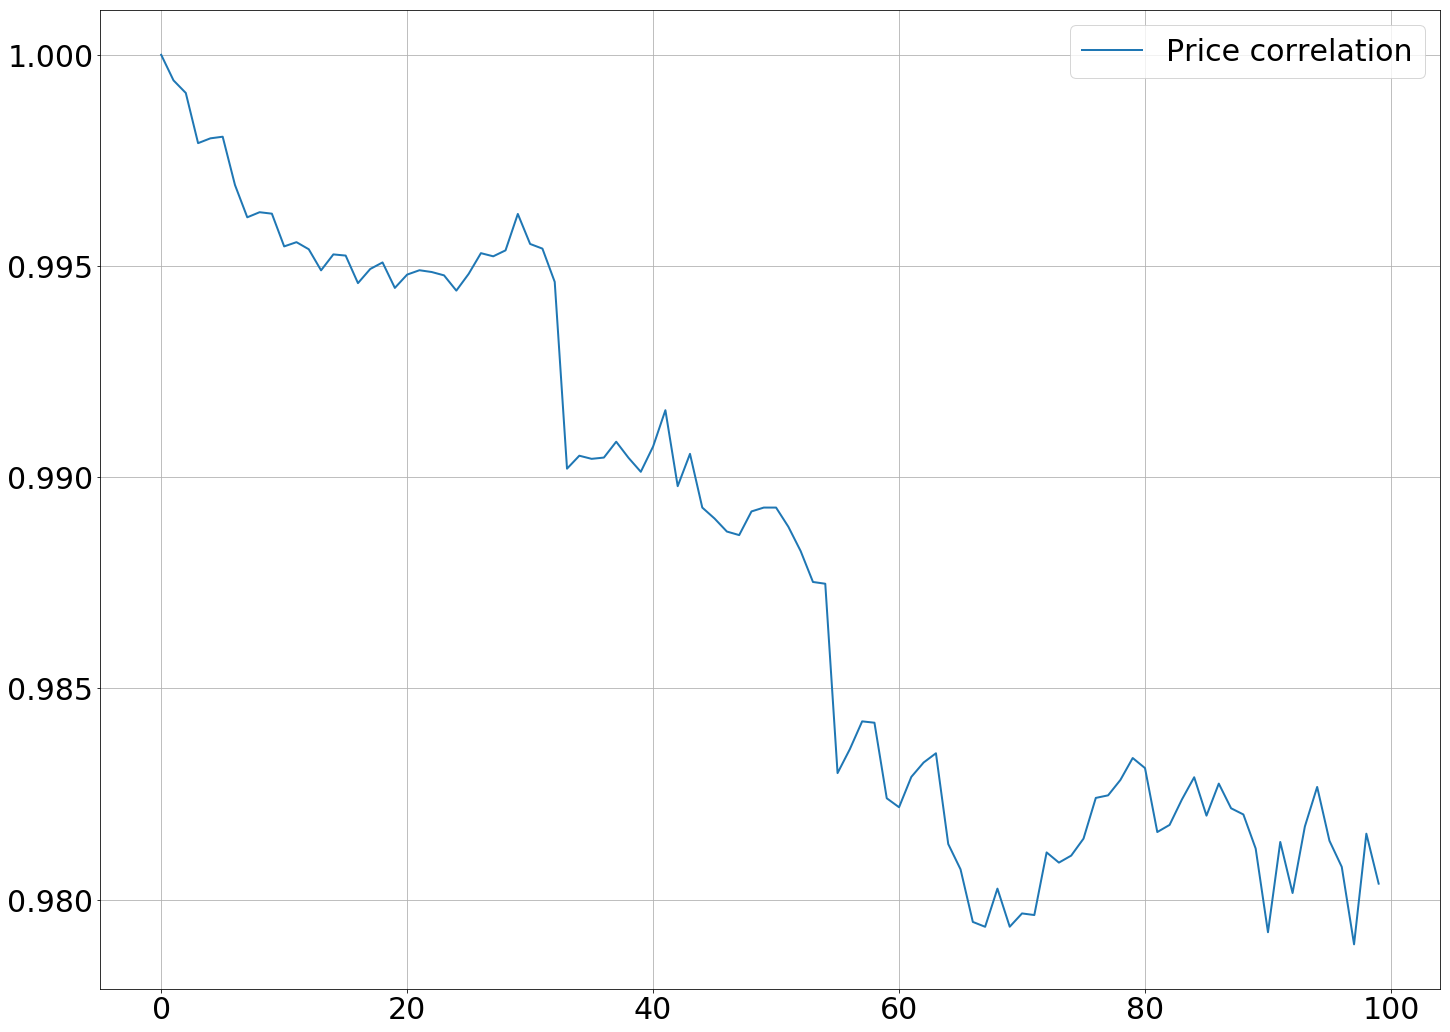
\includegraphics[width=\textwidth]{bidask-price-correlation}
        \caption{Correlation of order prices}
        \label{fig:bidask-price-correlation}
    \end{subfigure}
    \begin{subfigure}[b]{0.45\textwidth}
        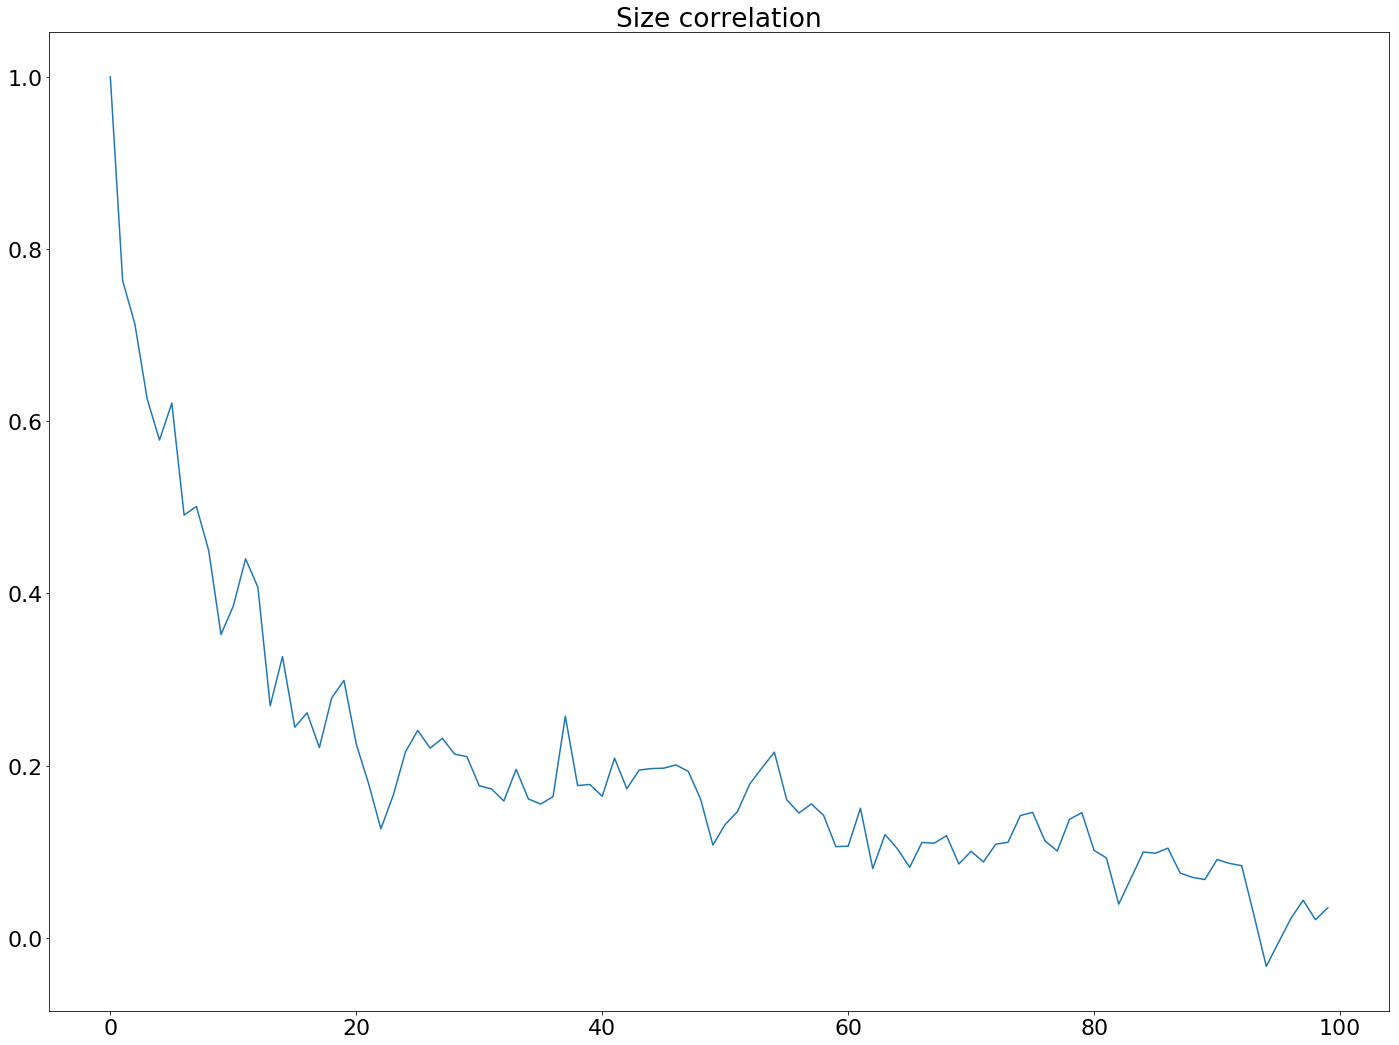
\includegraphics[width=\textwidth]{bidask-size-correlation}
        \caption{Correlation of order sizes}
        \label{fig:bidask-size-correlation}
    \end{subfigure}
    \caption{Correlation measured for 100 order book states}\label{fig:bidask-correlation}
\end{figure}

With this brief understanding of how limit levels $n$ affect order prices and sizes, we will try to make a statement about how order book states are related to the most recent state.
More precisely, we will determine the correlation between the order prices and sizes from the previous $m$ states and the most recent order book state.
We will take an average of 100 evaluations whereas we take a single order book state at time $t$ and a sequence of 100 previous order book states for each of which we measure the Shannon entropy\cite{shannon2001mathematical} to the state at $t$, whereas $n=40$ (maximum).
As can be seen in Figure \ref{fig:bidask-price-correlation}, the correlation of the price positions drop rapidly. However the effective change is not significant, indicating that the price changes are noticeable but overall do not differ much.
Order book states which lay more than 40 states in the past are slightly less correlated with the current state.
The correlation of order sizes, as shown in Figure \ref{fig:bidask-size-correlation} drops more rapidly and to a much greater extent than the order prices.
This indicates that traders choose a broad range of order sizes.
As a result, a window size of order book states $m$ greater than 40 states is suggested, in order to benefit from price differences within the feature.

\subsection{Feature: price and size of historical trades}
\label{sec:data-feature-2}
The previous feature provides information to the learner in order to reason about the hypotheses which are derived from orders placed and canceled.
In order to reason about whether or not trade events can provide a positive learning effect to the agent to optimize order placement, we construct a feature that covers the hypotheses \ref{sec:data-hypthesis-trade-price-volume} and partially \ref{sec:data-hypthesis-order-trade-volume-time}, as follows.
A $Trade$ (Eq. \ref{eq:trade}) carries an order side $os$, a quantity $q$ and a price $p$.
Similar to the previous feature, in this feature, we take $n$ trades into consideration, which occurred prior the time of the order placement.
More precisely, the feature is generated at some time $t$, when an order is placed, and therefore the time stamp $ts$ of the historical trades must satisfy $ts \leq t$.
\\
\\
A straightforward approach would be to construct the feature $s_{trade}$ as,
\begin{equation}
    s_{trade} =\begin{pmatrix}
        p_1 & q_1 & os_1 \\
        p_2 & q_2 & os_2 \\
        \vdots & \vdots & \vdots\\
        p_n & q_n & os_n \\
    \end{pmatrix}
    \ \forall \ p, q, os, ts \in Trade
\end{equation}, whereas $ts_n - ts_1 \leq m$.
However, trades do not occur at fixed time intervals and this causes the length of the vector to vary.
Accordingly, we calculate the time difference $\Delta{ts}$ between each historical trade and the subsequent historical trade.
For the most recent historical trade, the time difference is measured to the time of the order placement $t$.
That is,
\begin{equation}
    \Delta{ts}_i = \begin{cases}
    t - ts_i &\text{if i = 1}\\
    ts_{i+1} - ts_i &\text{otherwise}
    \end{cases}
\end{equation}

As a result we can redefine the feature $s_{trade}$, that is used by the learner as observation state, as,
\begin{equation}
    s_{trade} =\begin{pmatrix}
        \Delta{ts_1} & p_1 & q_1 & os_1 \\
        \Delta{ts_2} & p_2 & q_2 & os_2 \\
        \vdots & \vdots & \vdots & \vdots\\
        \Delta{ts_n} & p_n & q_n & os_n \\
    \end{pmatrix}
    \ \forall \ p, q, os, ts \in Trade
\end{equation}
\hfill
\\
\\
In addition, the new feature is normalized such that the prices are divided by the market price $p_t$ and the quantities are divided by the size of the order $q_t$ which is about to be placed at time $t$.
As a result, we constructed a feature vector of length $n$ (number of trades) that contains information about the price, order side and quantity of historical trades, as well as their order of occurrence.

\section{Conclusion}

Event data was collected from the Bittrex cryptocurrency exchange and a limit order book was reconstructed therefrom.
This limit order book serves as the historical data set and source for the match engine in order to simulate order placement. 
Subsequently the price chart, derived from the order book generated, was shown and the underlying event data were investigated.
Patterns were found which give insight into how market participants positioned their orders, with respect to price and size.
It was shown that the price movement was likely to be due to (1) an imbalance between bid and ask orders; (2) a distinctive way of posting or canceling orders; and (3) consecutive or impulsive trades.
These findings were incorporated within the two features constructed, and will serve as the observation state for the reinforcement learning agents that are described in the following chapter.
\chapter{Experimental Setup}

\section{Feature engineering}

\section{Execution Environment}

\section{Market making Environment}

\section{Q-Learning agent}

\section{Deep Q-Network agent}

\chapter{Evaluation procedure and discussion of results}
\label{chap:analysis}

In the previous Chapter, we built a reinforcement learning environment with the use of the components which were described earlier, in Chapter \ref{chap:preliminaries}.
The environment facilitates the simulation of order placement on historical order books of the type described in Chapter \ref{chap:data}.
Furthermore, two agents were introduced: a Q-Learner which learns on private variables; and a Deep Q-Network which learns on market variables.

The aim of this chapter is to make use of this setup and to run simulations, thereby observing whether or not reinforcement learning is indeed capable of optimizing the placement of limit orders.
Therefore, a comprehensive evaluation procedure will be introduced that  measures the capabilities of the reinforcement learning agents.
Throughout this process, real world historical order books will be drawn upon, as well as artificially created order books, where the latter define distinct price trends and eliminate the noise present in real market data.
We first outline the steps of the evaluation procedure.
Subsequently, the real world data sets chosen and their use within the reinforcement learning setup will be described.
Finally, we will evaluate the steps taken in respect of the order that will be used for illustrative purposes.
Accordingly, this chapter will seek to quantify the effectiveness of deep reinforcement learning and its use of the market features previously constructed.

\section{Explanation of the evaluation procedure}
\label{sec:analysis-procedure}
This section explains the evaluation procedure that will be elaborated in the following sections of this chapter. From our analysis of the same, we will aim to formulate a statement that expresses the capabilities of optimizing limit order placement with reinforcement learning and the use of raw market data.
The evaluation steps will proceed chronologically, as follows:
\begin{description}
    \item[Empirical investigation: ]
    Section \ref{sec:eval-empirical} investigates the reinforcement learning environment empirically by simulating an agent's behaviour that places buy and sell orders for a range of limit levels.
    This will provide knowledge about the limitations of the potential optimization possibilities within the given data set and how well we can expect the reinforcement learners to perform.
    More precisely, we determine the \textit{expected returns} for (1) the optimally chosen limit order and (2) an immediate purchase or sale by using a market order.
    
    \item[Q-Learning agent policy: ]
    In Section \ref{sec:eval-qlearn}, we make an attempt to build an order placement policy based on private variables only, by using the Q-Learner.
    This will provide insights into the performance of a naive reinforcement learner and serve as a benchmark for the following simulations proceeded in which we consider market variables.
    Thereby, we observe the \textit{average reward} achieved by the Q-Learning agent that uses private variables.

    \item[DQN agent policy: ]
    Section \ref{sec:eval-dqn} applies market variables to the DQN agent.
    Hereby, we make use of Feature I: the price and size of historical orders as described in Chapter \ref{chap:data} (Section \ref{sec:data-feature-1}); as well as Feature II: the price and size of historical trades (described in Section \ref{sec:data-feature-2}).
    As in the previous evaluation step, we will find the average rewards produced by the agent.
    More precisely, we determine the average rewards for the DQN agent with the use of private variables and (1) historical orders or (2) historical trades.

    \item[DQN agent limitations: ]
    Section \ref{sec:eval-dqn-limitations} aims to determine the capabilities and limitations of the DQN agent in greater detail.
    We investigate the actions selected by the agent in order to determine the agent's limitations.
    In addition, we apply the agent to an environment which is equipped with an artificially generated order book and will enable us to determine to which extent the agent is able to learn from certain price trends.
    The results achieved in this evaluation step are (1) \textit{the discovery} of situations where the DQN agent does not perform well and (2) the \textit{average reward} achieved by using order books that follow an artificially created trend (downwards and sine curve).
\end{description}
With the results obtained throughout this evaluation, we will be able to determine and quantify the extent to which deep reinforcement learning can optimize limit order placement; we will also be able to give reasons for its limitations.

\section{Data sets and their usage in the reinforcement learning setup}
\label{sec:analysis-data-sets}
We have selected two $\sim$30 minute samples of historical order book recordings for the experiments in this chapter.
One of the reasons for choosing two very different data sets is to determine the ability of the learners to react to a variety of market situations.
In addition, as explained in the following section, the expected return of a learner for buying and selling assets heavily depends on the market price movements and therefore the behaviour is expected to be different for the data sets in use.
More precisely, \textit{data set I}, as shown in Figure \ref{fig:sample-down-price}), is a downward trend (indicated by the bid/ask mid-price) and consists of 1132 order book states with an overall duration of 1681.8 seconds, resulting in 0.67 states per second.
In contrast, \textit{data set II}, as shown in Figure \ref{fig:sample-up-price}, consists of 1469 order book states with an overall duration of 1746.0 seconds, resulting in 0.84 states per second, which indicates that there was slightly more pressure in terms of orders placed and canceled in this data set.
When reinforcement learning is applied, the data sets are split with ratio $2:1$, resulting in a training set of $\sim$20 minutes and a test set of $\sim$10 minutes.
Although more than two data sets would produce a more generalized outcome of this evaluation, this was computationally not feasible within this work.
\begin{figure}[H]
    \centering
    \begin{subfigure}[b]{0.45\textwidth}
        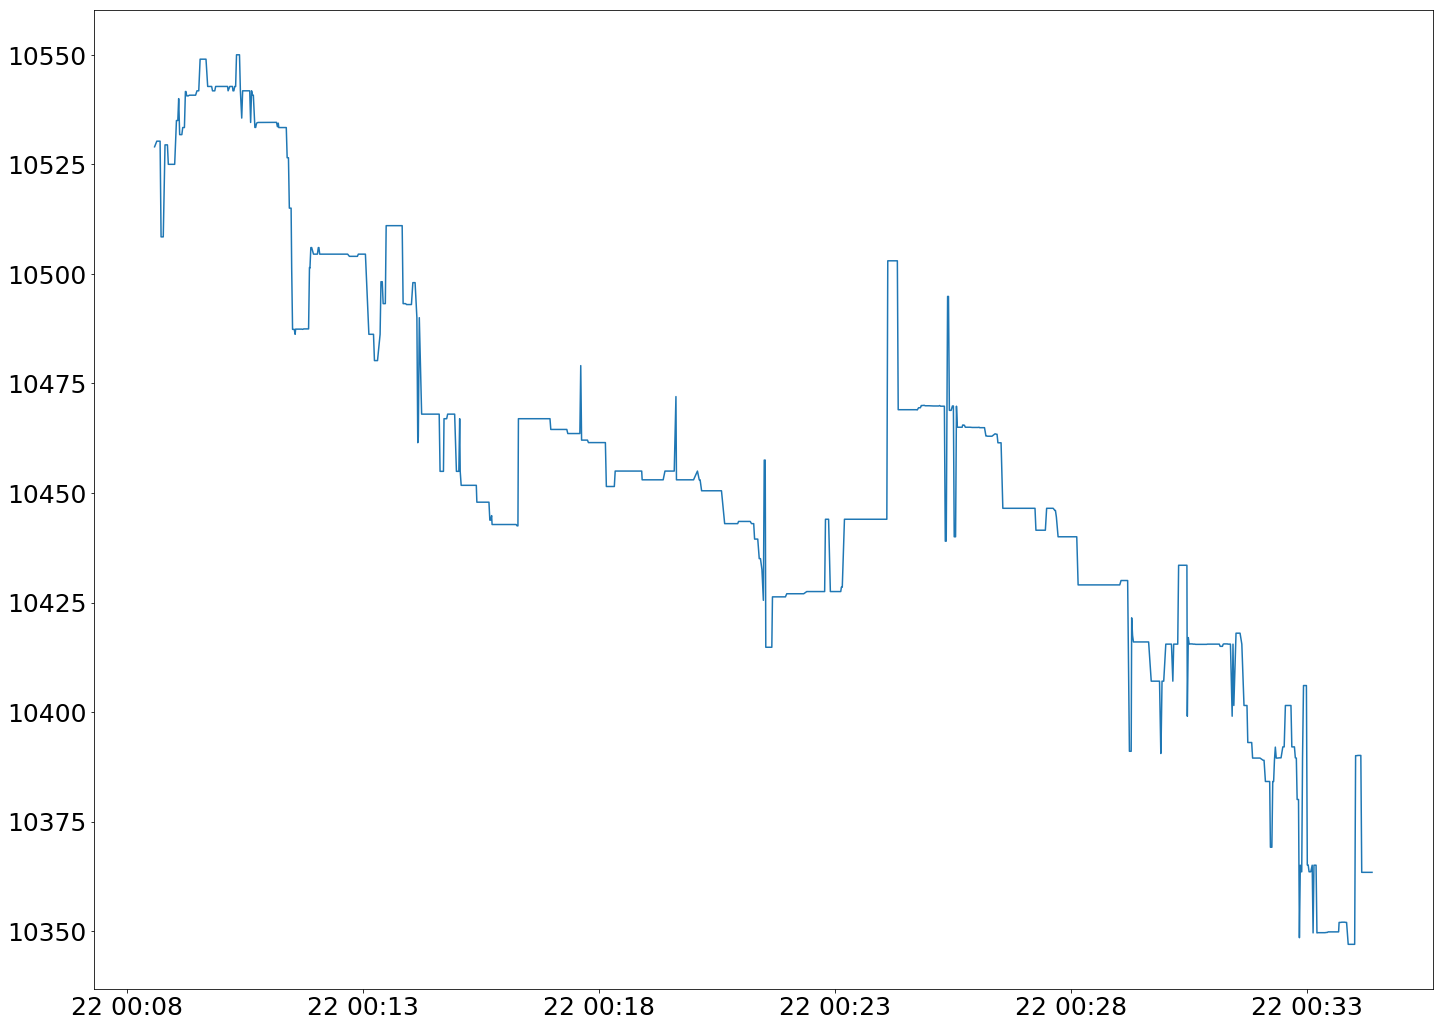
\includegraphics[width=\textwidth]{sample-down-price}
        \caption{30 minute downwards trend}
        \label{fig:sample-down-price}
    \end{subfigure}
    \begin{subfigure}[b]{0.45\textwidth}
        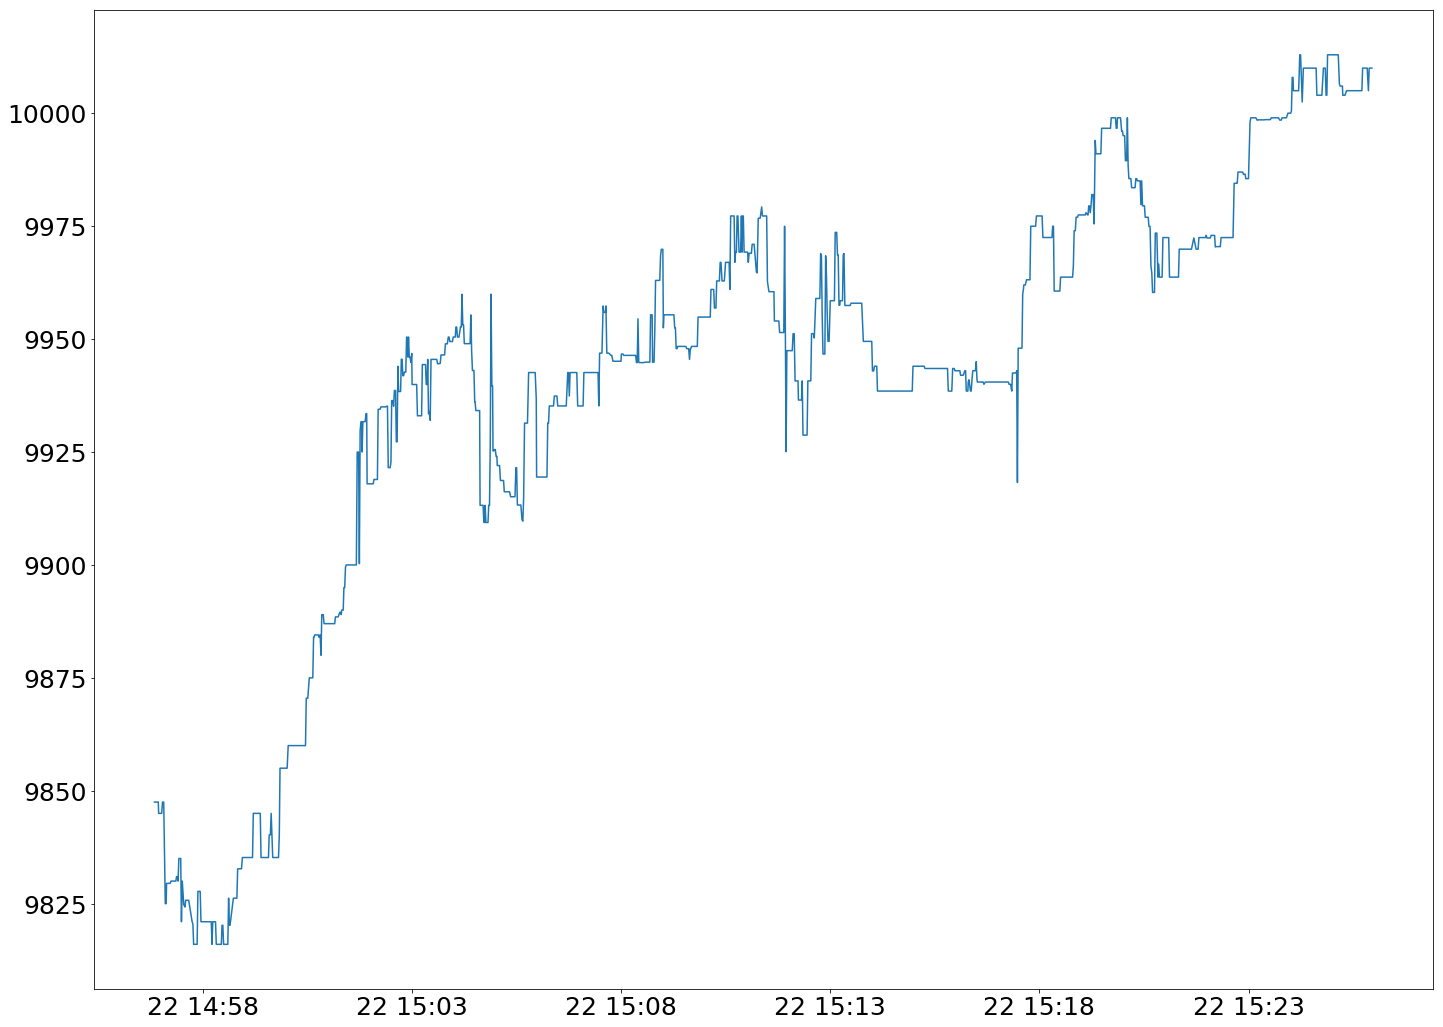
\includegraphics[width=\textwidth]{sample-up-price}
        \caption{30 minute upwards trend}
        \label{fig:sample-up-price}
    \end{subfigure}
    \caption{Bid/ask mid-price of 30 minute order book recordings.}
    \label{fig:sample-price}
\end{figure}

As explained in Chapter \ref{chap:setup}, the historical data sets are not maintained by the reinforcement learning agents directly but instead by the reinforcement learning environment.
The environment provides an observation state $O$, derived from the data set, to an agent, after which the agent decides to take an action $a$ in the form of a limit level.
In turn, the environment prices the order at the received price level and returns the evaluated reward $r$ and the next observation state $O$ to the agent.
In this way, the agent can simulate the placement of limit orders in such a way that, within the given time horizon $H$, the inventory can be either bought or sold.
For each \textit{epoch} an agent processes, one order, with a specified inventory and time horizon, is defined and is to be filled.
Therefore, the reinforcement learning environment selects, for each epoch the agent initiates, a range of order book states which form the given time horizon $H$ within which the agent is supposed to complete an order.
\begin{figure}[H]
    \centering
    \makebox[\linewidth]{
        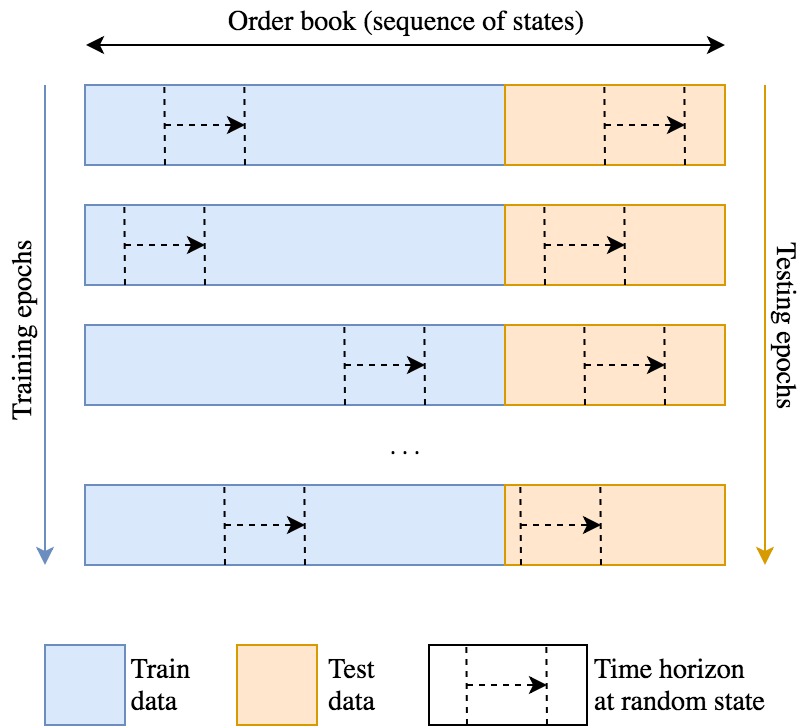
\includegraphics[width=8cm]{images/evaluation-orderbook.png}
    }
    \caption{Order placement training and testing on an order book data set.}
    \label{fig:eval-orderbook-window}
\end{figure}
Figure \ref{fig:eval-orderbook-window} illustrates this process.
A randomly-chosen order book state defines the beginning of the time horizon and the set of order book states that fall into this window.
This is very crucial since the states within this time horizon and the set of states, not only leads to the observation states received by the agent, but also will determine the outcome of the matching process.
More precisely, for each step the agent takes, a consecutive sequence of order book states (with time stamp difference of $\Delta{t}$) will be considered by the match engine, as explained in the previous chapter in Section \ref{setup:parameters}.
This process is identical for testing, except that the underlying data is different and the agent will not learn from the epochs proceeded during testing and instead will report the achieved rewards.

\section{An empirical investigation of the reinforcement learning environment}
\label{sec:eval-empirical}
In this section, the relationship between the limit order placement and the received return will be investigated.
The methods demonstrated are based on the related work described in Section \ref{sec:related-execution-behaviour} and provide the ability to empirically evaluate the reinforcement learning environment (Chapter \ref{chap:setup}).
Therefore, we simulate an agent that submits actions in order to buy and sell shares at every possible limit level and records the immediate returns it receives.
A return is defined as the difference between the market price prior to the order placement and the volume- weighted average price (VWAP) paid or received, as stated in Eq. \ref{setup:reward}.
As a result, we gain an understanding of the estimated rewards of limit order placement using the given historical data set.
In addition, these results set a benchmark for the reinforcement learners to come.

We will now describe the setup of this investigation.
We investigate the rewards of limit orders placed on progressively increasing time horizons, from 10 seconds to 100 seconds, and thereby observe the importance of the action chosen by the agents in order to buy or sell assets, in accordance with the length of the time horizon.
For each time horizon, we place (e.g. cross-validating) 100 orders of size 1.0 BTC at the beginning of the time horizon whose beginning is defined by a randomly-chosen order book state. 
A market order follows for the remainder of shares (if any) once the time horizon is consumed.
The expected return is then derived from the average of the received returns of these 100 orders.
This process is repeated across a range of 201 actions $A$ that correspond to the limit levels $-100...100$ with step size $\Delta{a} = \$0.10$, resulting in orders priced in the range of $p_m-10 \ \dots \ p_m+10$, whereas $p_m$ is the market price before the order was placed.
The limit levels are chosen broadly in order to retrieve understanding about the outcome of a variety of possible actions.
Hence, a total of 20,100 orders are submitted for each time horizon defined.
Finally, the investigation is undertaken for both data sets I and II.

\subsection{Order placement behavior on data set I}
For data set I, where the market sees a downwards trend, the intuition is as follows:
We expect buy orders to result in better returns when placed deep in the order book, in other words, on orders that have a highly negative limit level ($a<0$).
Since the price tends to fall, the assumption is that an agent is able to buy at a lower price once time has passed.
Therefore, the longer the time horizon, the lower the limit level that can still be chosen in order to execute the full amount of shares.
In contrast,  we expect sell orders to provide better returns when the agent crosses the spread with a positive limit level ($a>0$).
The assumption is that, in a falling market, it is unlikely that market participants are willing to buy at higher prices and therefore the agent must place sell orders higher in the book in order to sell immediately.
Otherwise, the longer the time horizon, the less return an agent would retrieve as the market order, that is submitted if the order has not been filled, becomes costly.
This investigation is shown in Figure \ref{fig:behvaiour-down} for time horizons of 10, 30, 60 and 100 seconds.
The x-axis indicates the placement of the order at limit levels ranging from $a=-100$ to $a=+100$ and the y-axis indicates the average return received.

With a time horizon of only 10 seconds left, the expected behavior is, however, proven wrong.
For buy orders, shown in Figure \ref{fig:behvaiour-down-10s-buy}, the returns suggest that orders be placed close to the spread, but still on the opposing side ($a=\sim{5}$).
The spike at limit level $a=\sim{-5}$ indicates that the overall best return was produced at this level. However, this comes with the risk that the orders fail to execute, which is indicated by the downward spike also close to level $\sim{-5}$.
For selling within 10 seconds, as shown in Figure \ref{fig:behvaiour-up-10s-sell}, the best return is given when crossing the spread with a positive limit level with $a=\sim{+50}$.

With an increased time horizon of a total of 30 seconds, as shown in Figures \ref{fig:behvaiour-down-30s-buy} and \ref{fig:behvaiour-down-30s-sell}, the expected behavior becomes more apparent.
Positive returns can be achieved by posting buy orders deep in the order book.
Therefore, we can expect that in the given market situation, an agent would be able to partially execute the order at very low limit levels and, for the unexecuted part, a market order would follow.
The densest range of positive returns can be seen around the limit levels just below the spread.
Orders placed deeper in the book oftentimes result in slightly lower returns, which indicates that the orders were only filled partially and expensive market orders followed.
Crossing the spread causes increasingly lower returns, the more positive the limit level is chosen, as a result of agents' willingness to immediately buy at an increasing price.
The opposite effect occurs while selling assets.
Market orders higher in the book result in better returns than limit orders deep in the book.
Interestingly, orders which were placed very deep in the book, at limit level $\sim$-50 and below, are rewarded better than the ones close to the spread.
The most likely reasons it that a minority of orders  were partially filled at this level during the cross-validation process.

With time horizons of 60 and 100 seconds, the expected behavior of the orders is clearly apparent.
Buy orders, as shown in Figures \ref{fig:behvaiour-down-60s-buy} and \ref{fig:behvaiour-down-100s-buy}, achieve highest returns when placed very deep in the order book.
However, when placed at levels -100, the returns are slightly lower as a result of unexecuted orders which had to be completed with market orders.
In addition, positive limit levels become stable at this range since there are more sellers in the market with the extended time horizon.  Therefore, very highly placed orders have the same effect as limit orders posted only slightly above the spread.
Furthermore, placing orders very deep in the book has the same effect as when placing them just below the spread; that is, there are no traders willing to buy at such a high price and therefore market orders follow once time has passed.
\vfill
\newpage
\begin{figure}[H]
    \centering
    \begin{subfigure}[b]{0.45\textwidth}
        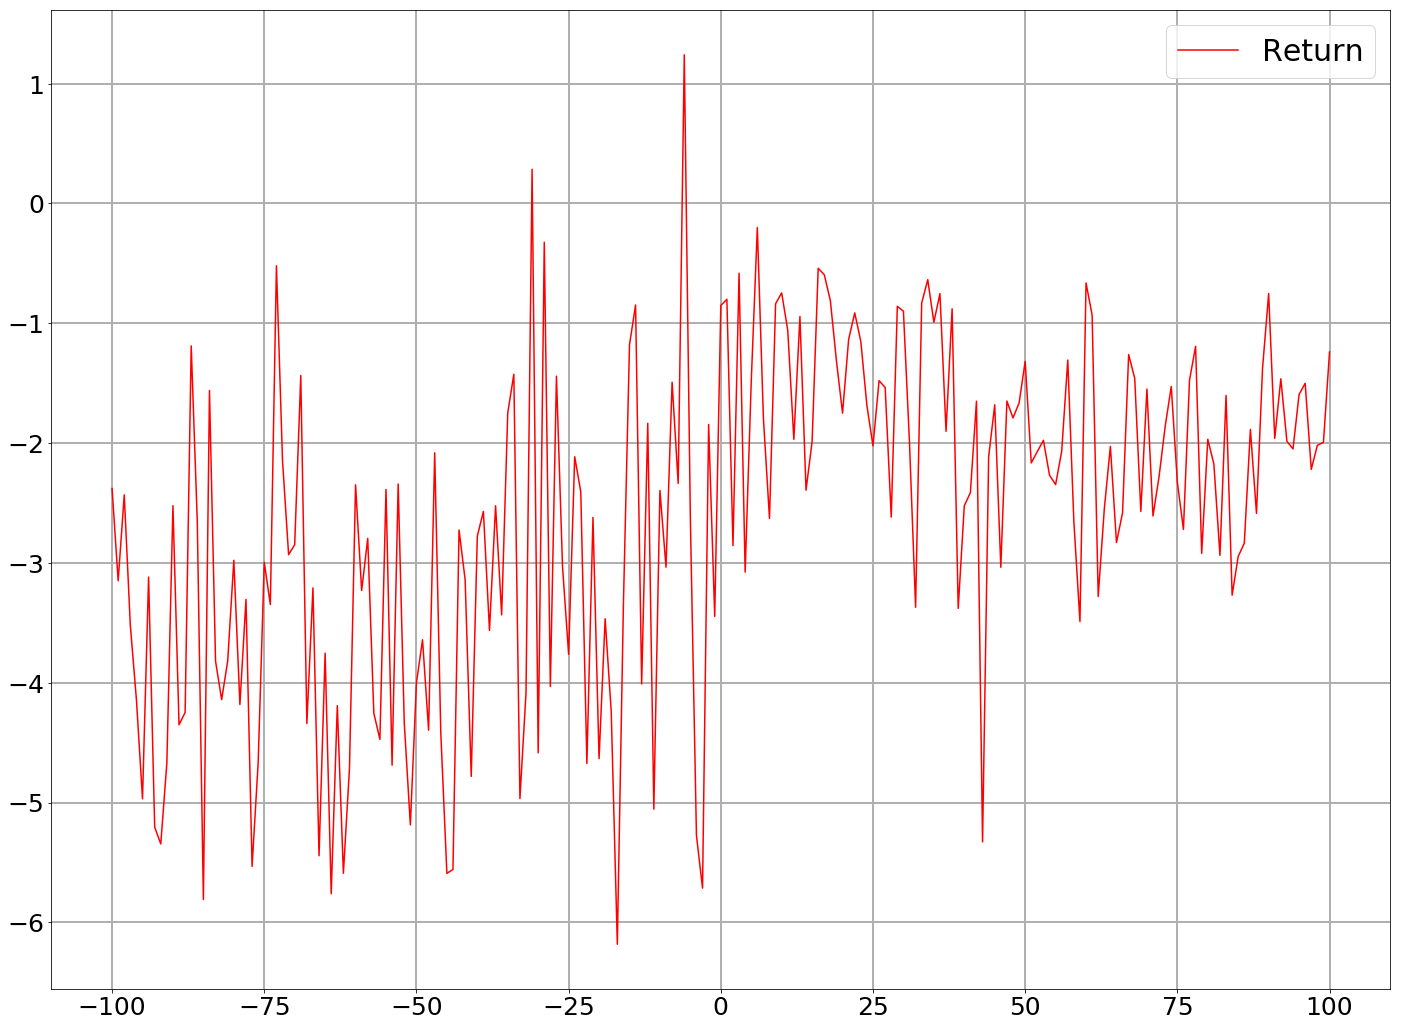
\includegraphics[width=\textwidth]{images/behaviour-10s-buy.png}
        \caption{Returns of buy orders within 10 seconds}
        \label{fig:behvaiour-down-10s-buy}
    \end{subfigure}
    \begin{subfigure}[b]{0.45\textwidth}
        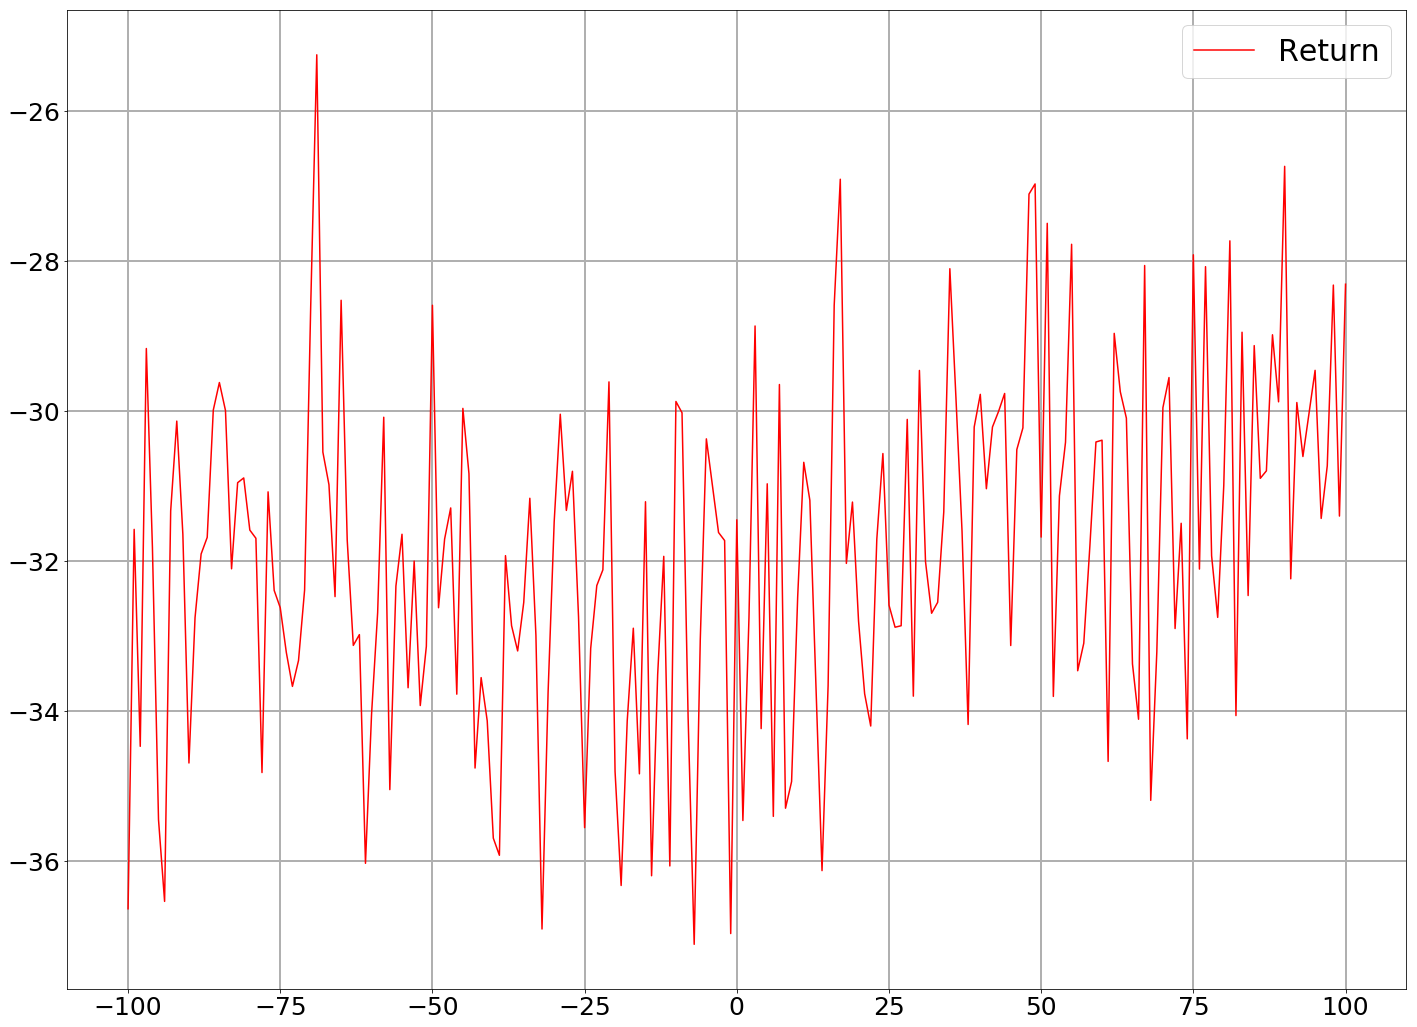
\includegraphics[width=\textwidth]{images/behaviour-10s-sell.png}
        \caption{Returns of sell orders within 10 seconds}
        \label{fig:behvaiour-down-10s-sell}
    \end{subfigure}
    \begin{subfigure}[b]{0.45\textwidth}
        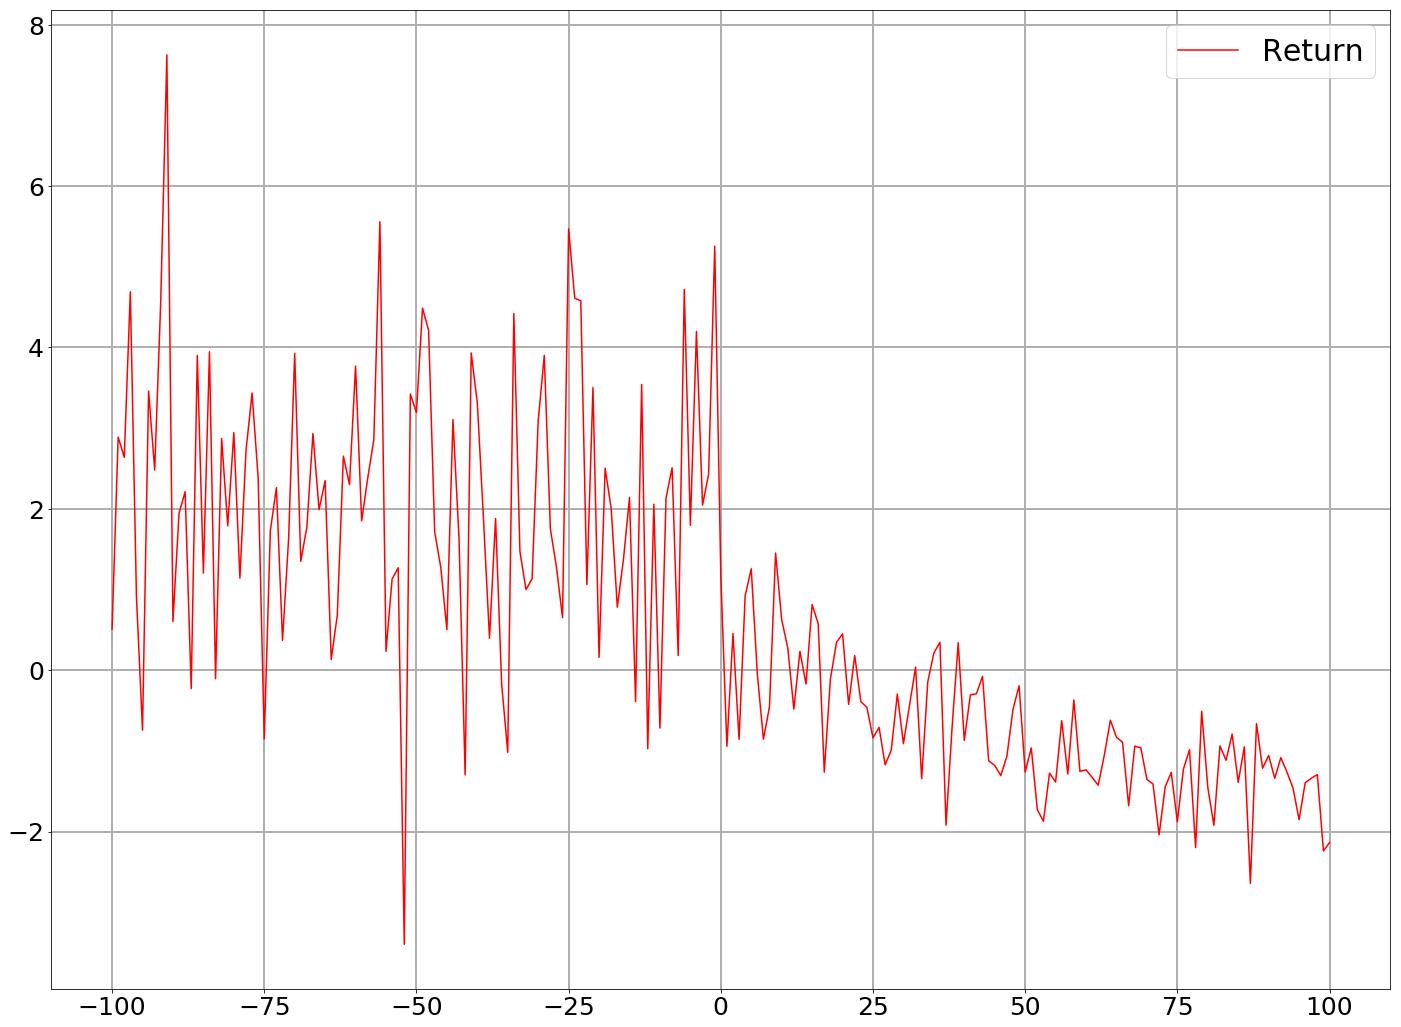
\includegraphics[width=\textwidth]{images/behaviour-30s-buy.png}
        \caption{Returns of buy orders within 30 seconds}
        \label{fig:behvaiour-down-30s-buy}
    \end{subfigure}
    \begin{subfigure}[b]{0.45\textwidth}
        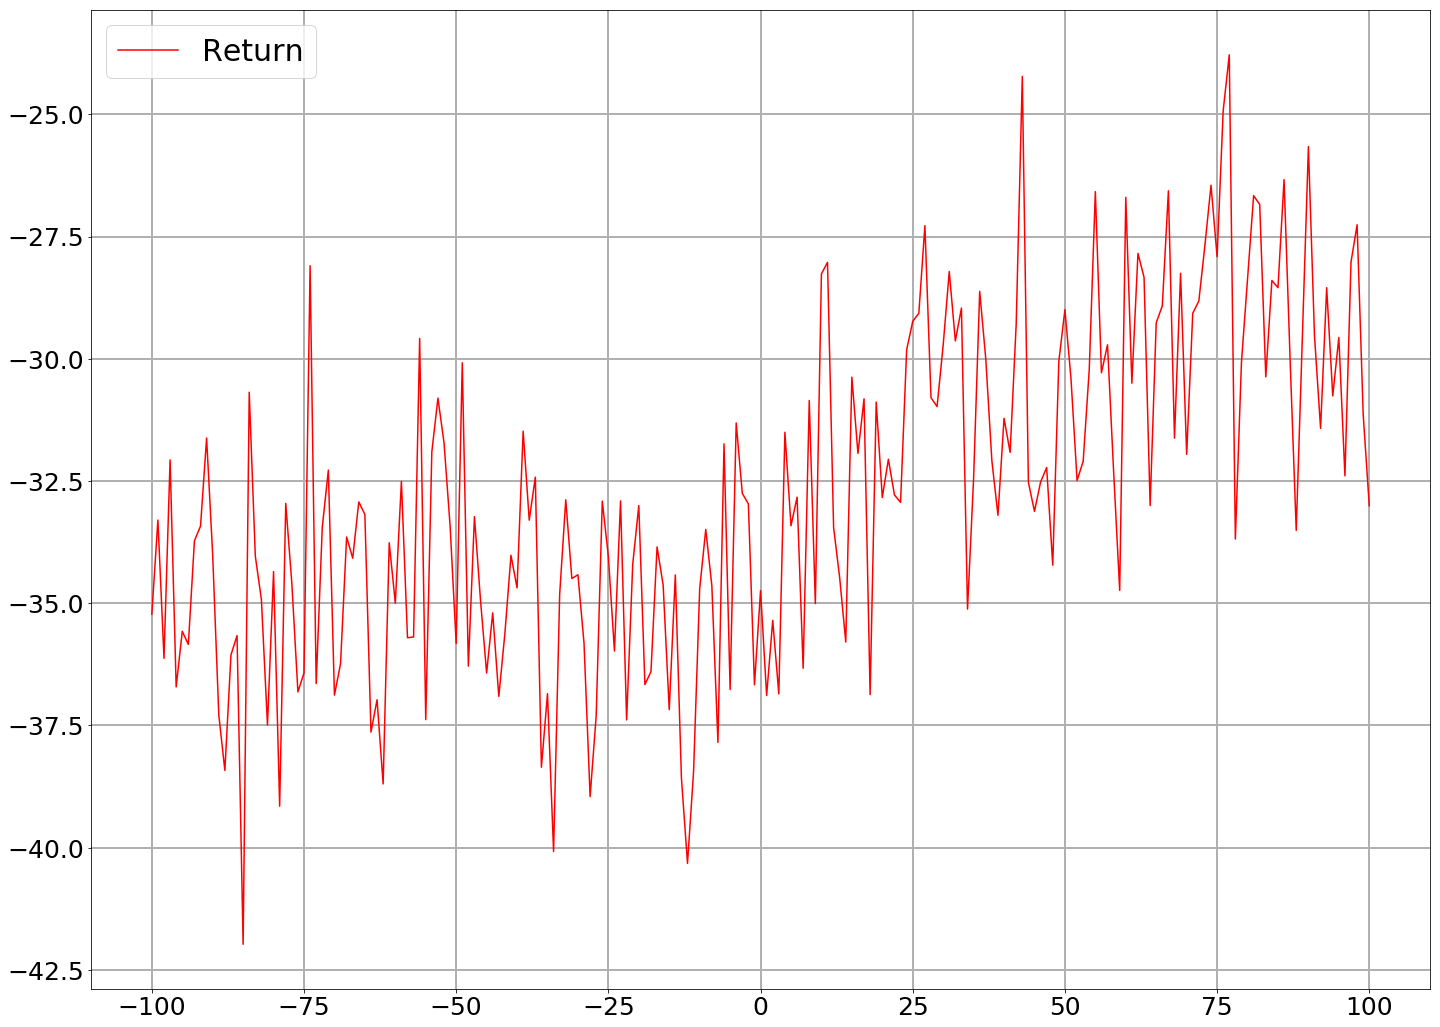
\includegraphics[width=\textwidth]{images/behaviour-30s-sell.png}
        \caption{Returns of sell orders within 30 seconds}
        \label{fig:behvaiour-down-30s-sell}
    \end{subfigure}
    \begin{subfigure}[b]{0.45\textwidth}
        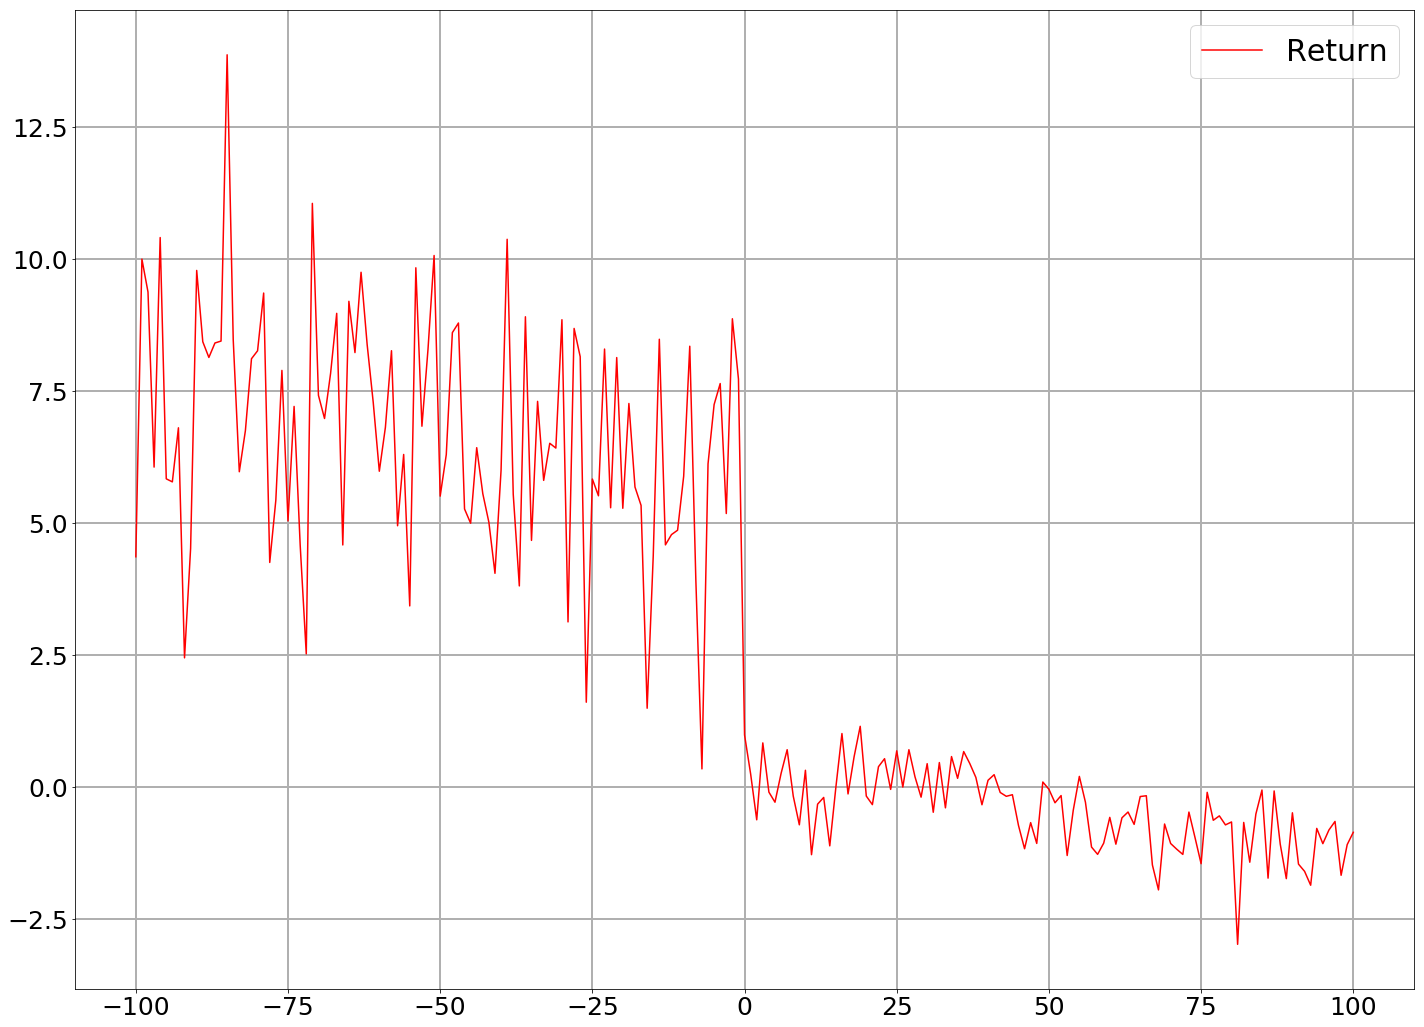
\includegraphics[width=\textwidth]{images/behaviour-60s-buy.png}
        \caption{Returns of buy orders within 60 seconds}
        \label{fig:behvaiour-down-60s-buy}
    \end{subfigure}
    \begin{subfigure}[b]{0.45\textwidth}
        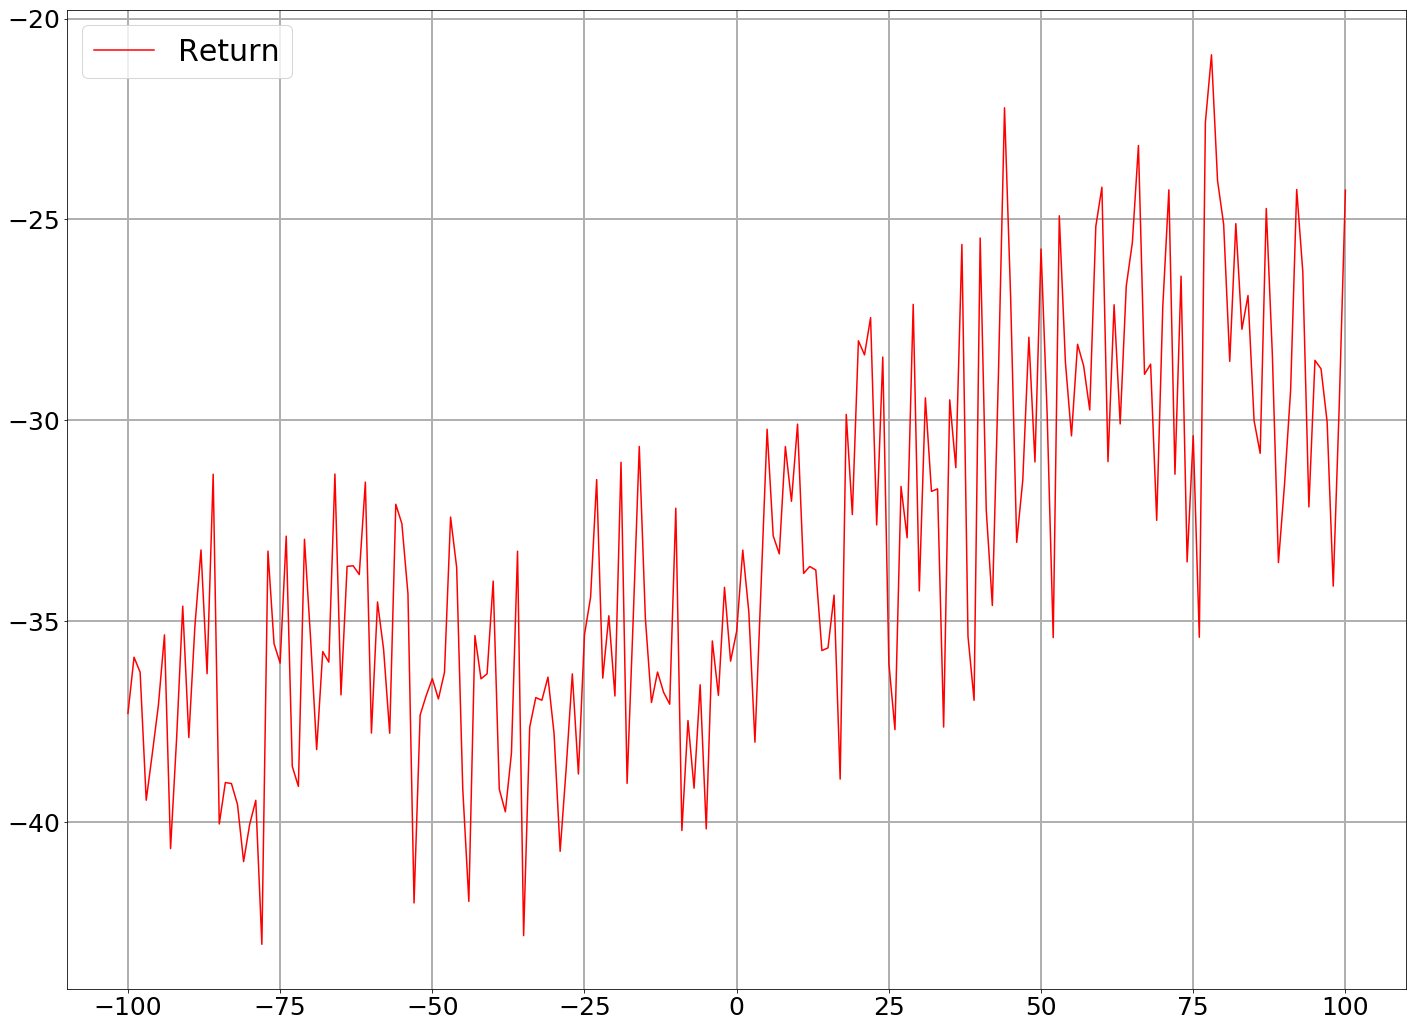
\includegraphics[width=\textwidth]{images/behaviour-60s-sell.png}
        \caption{Returns of sell orders 60 seconds}
        \label{fig:behvaiour-down-60s-sell}
    \end{subfigure}
    \begin{subfigure}[b]{0.45\textwidth}
        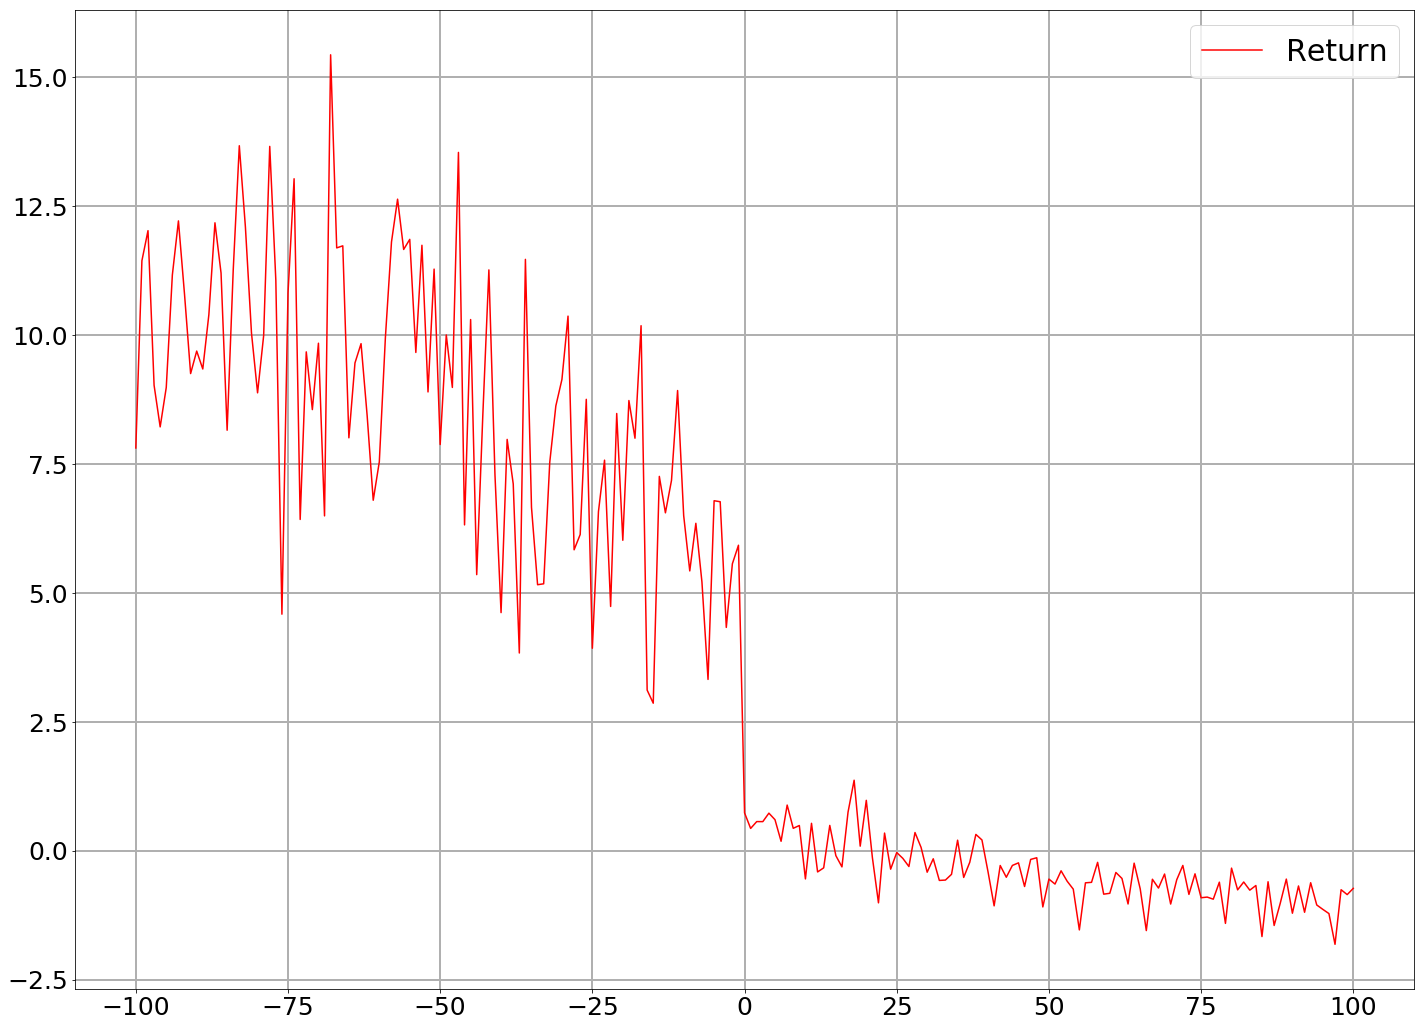
\includegraphics[width=\textwidth]{images/behaviour-100s-buy.png}
        \caption{Returns of buy orders 100 seconds}
        \label{fig:behvaiour-down-100s-buy}
    \end{subfigure}
    \begin{subfigure}[b]{0.45\textwidth}
        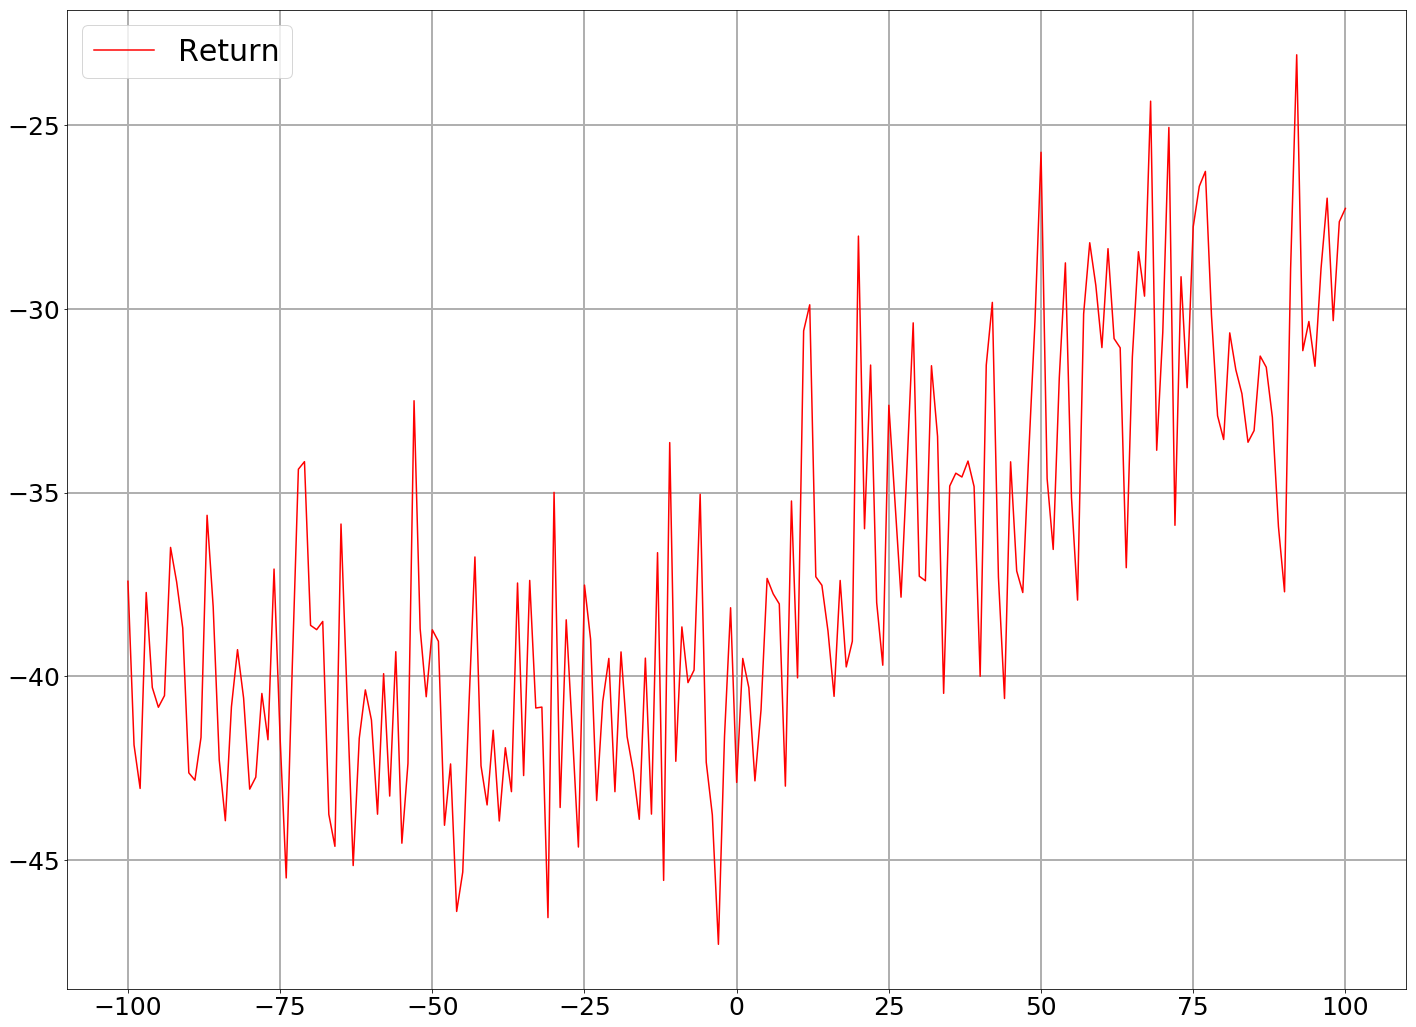
\includegraphics[width=\textwidth]{images/behaviour-100s-sell.png}
        \caption{Returns of sell orders 100 seconds}
        \label{fig:behvaiour-down-100s-sell}
    \end{subfigure}
    \caption{Returns of buy and sell orders executed within 10, 30, 60 and 100 seconds on data set I.}
    \label{fig:behvaiour-down}
\end{figure}

\begin{figure}[H]
    \centering
    \begin{subfigure}[b]{0.45\textwidth}
        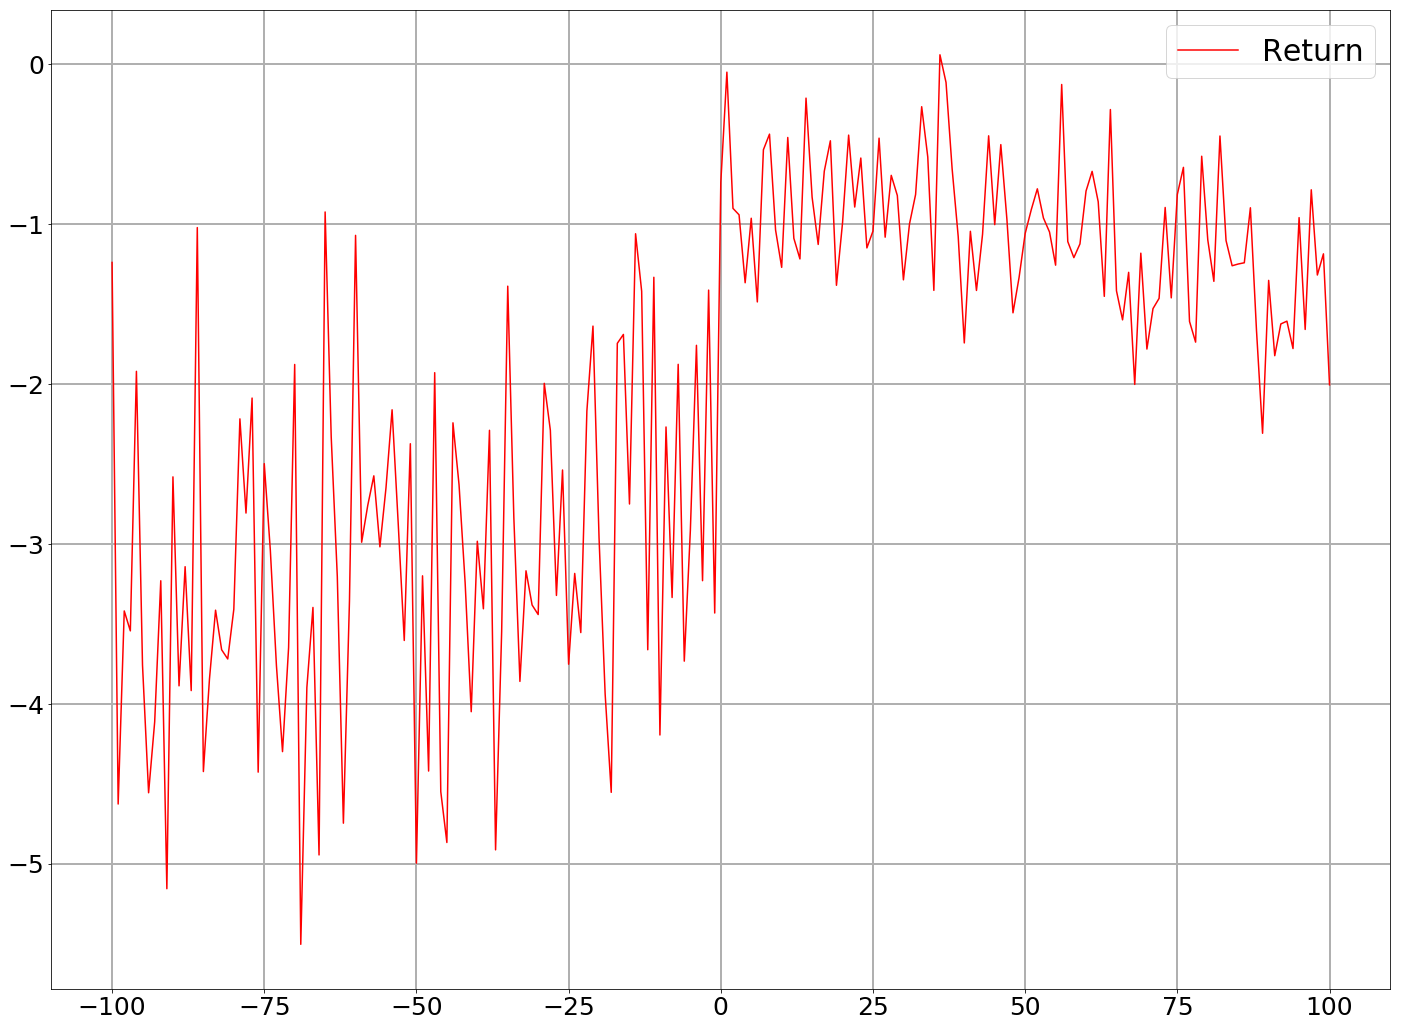
\includegraphics[width=\textwidth]{images/behaviour-up-10s-buy.png}
        \caption{Returns of buy orders within 10 seconds}
        \label{fig:behvaiour-up-10s-buy}
    \end{subfigure}
    \begin{subfigure}[b]{0.45\textwidth}
        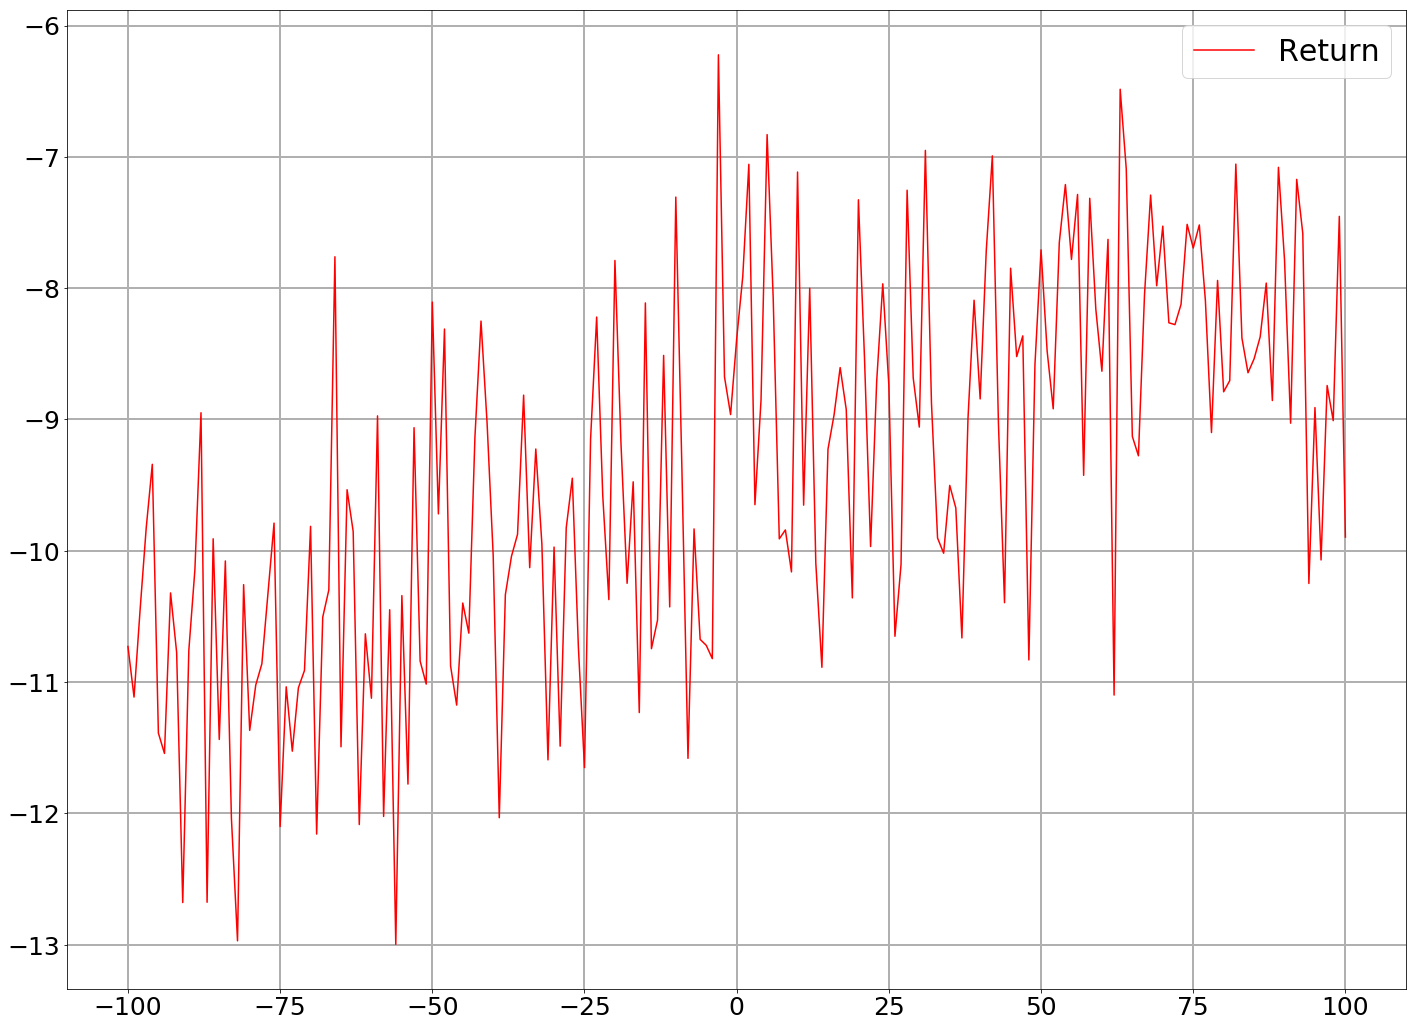
\includegraphics[width=\textwidth]{images/behaviour-up-10s-sell.png}
        \caption{Returns of sell orders within 10 seconds}
        \label{fig:behvaiour-up-10s-sell}
    \end{subfigure}
    \begin{subfigure}[b]{0.45\textwidth}
        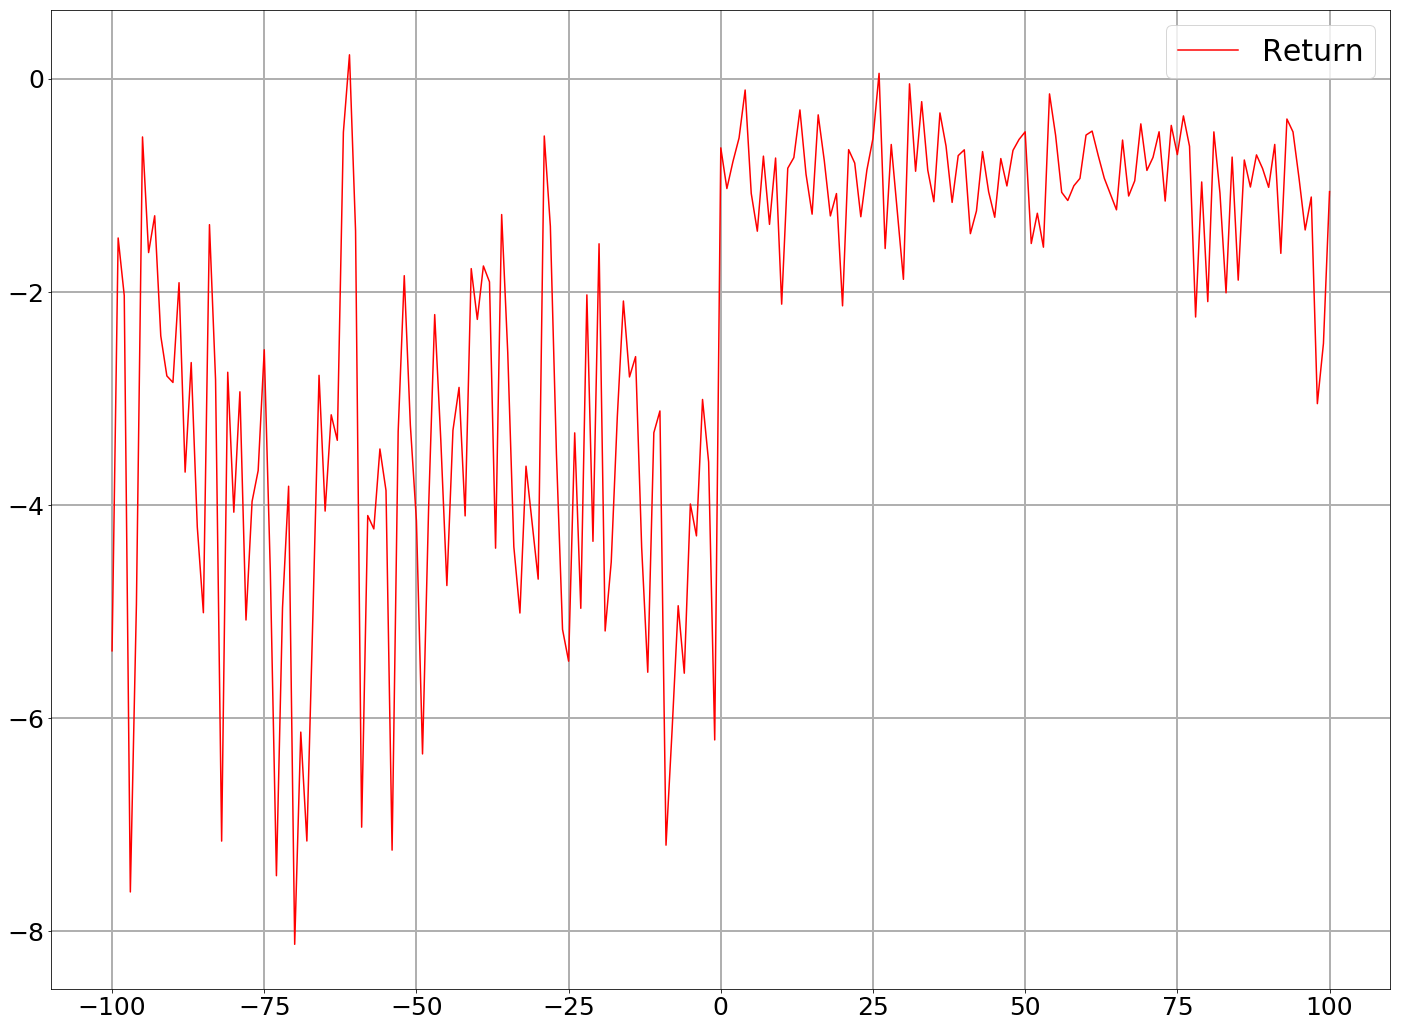
\includegraphics[width=\textwidth]{images/behaviour-up-30s-buy.png}
        \caption{Returns of buy orders within 30 seconds}
        \label{fig:behvaiour-up-30s-buy}
    \end{subfigure}
    \begin{subfigure}[b]{0.45\textwidth}
        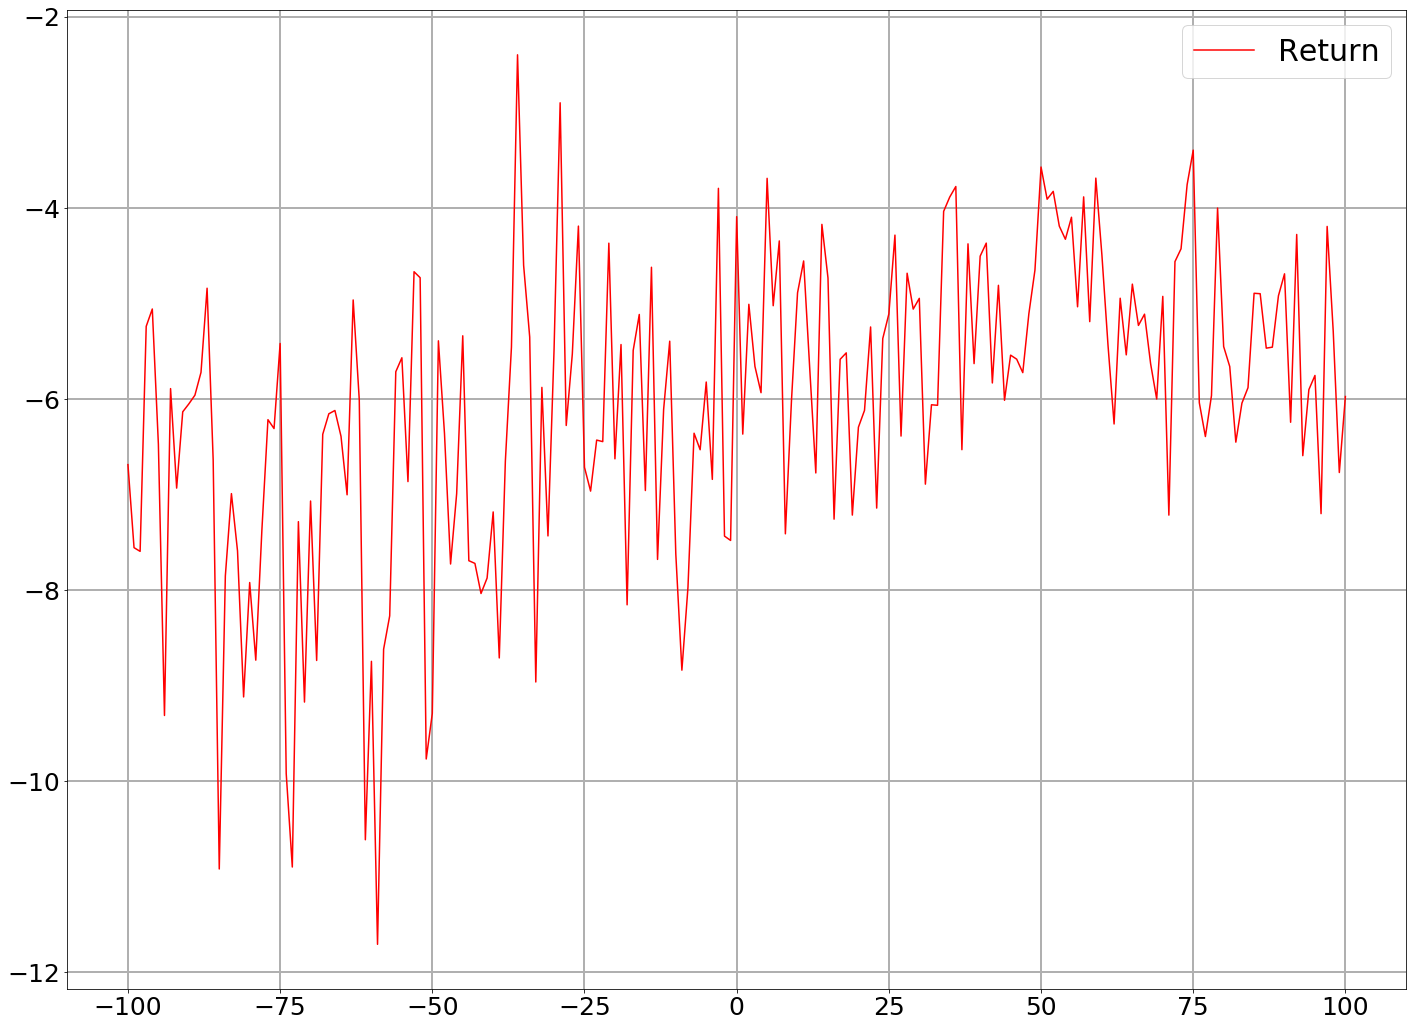
\includegraphics[width=\textwidth]{images/behaviour-up-30s-sell.png}
        \caption{Returns of sell orders within 30 seconds}
        \label{fig:behvaiour-up-30s-sell}
    \end{subfigure}
    \begin{subfigure}[b]{0.45\textwidth}
        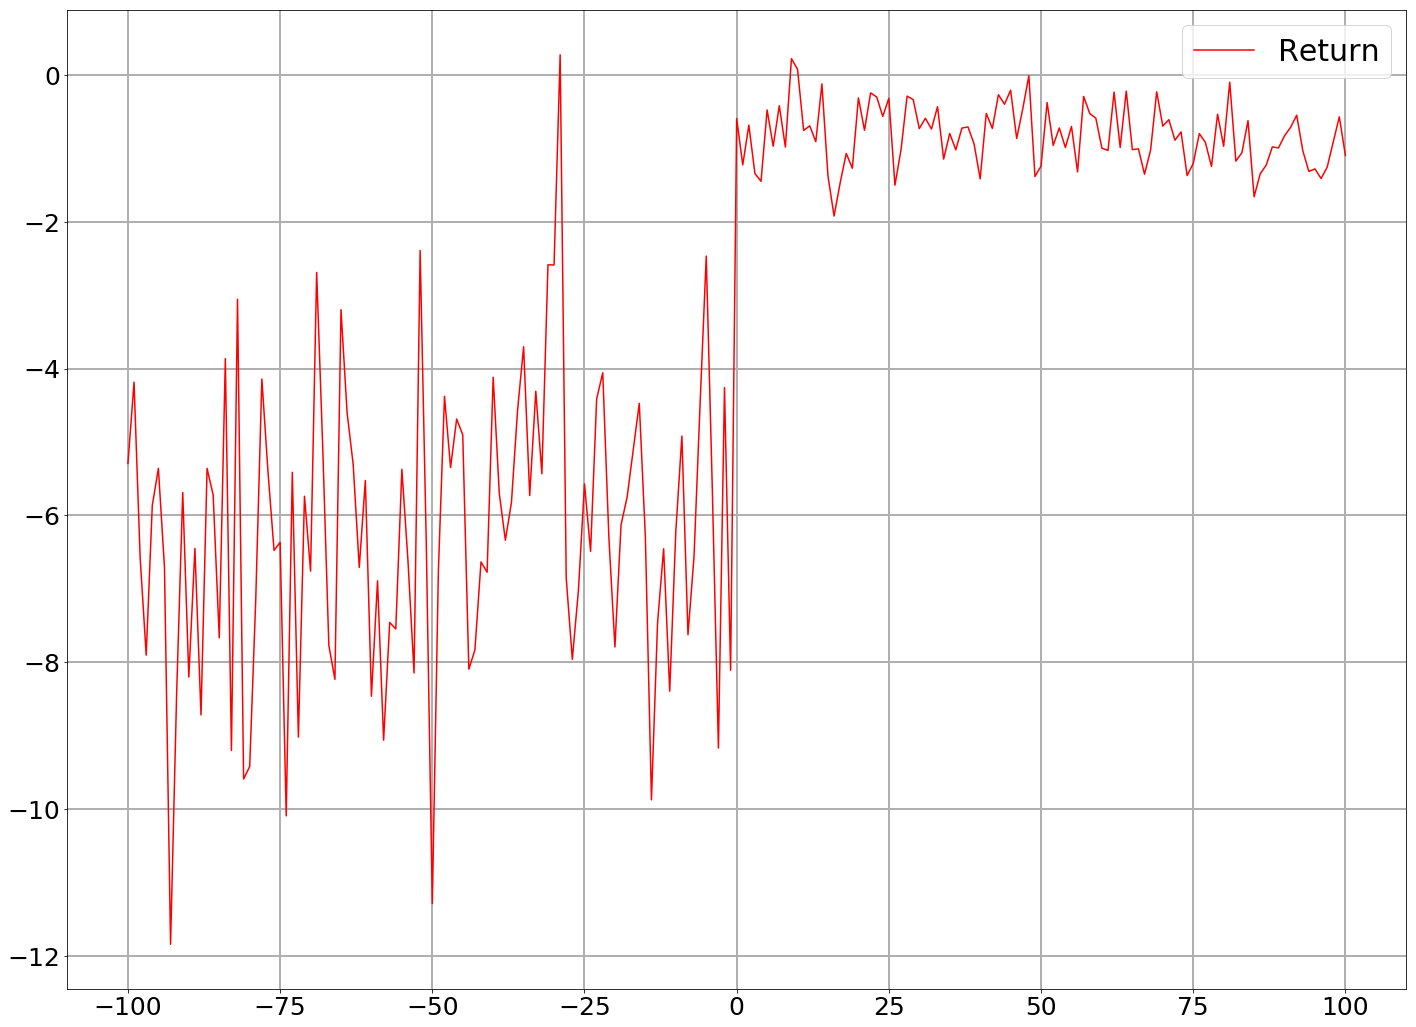
\includegraphics[width=\textwidth]{images/behaviour-up-60s-buy.png}
        \caption{Returns of buy orders within 60 seconds}
        \label{fig:behvaiour-up-60s-buy}
    \end{subfigure}
    \begin{subfigure}[b]{0.45\textwidth}
        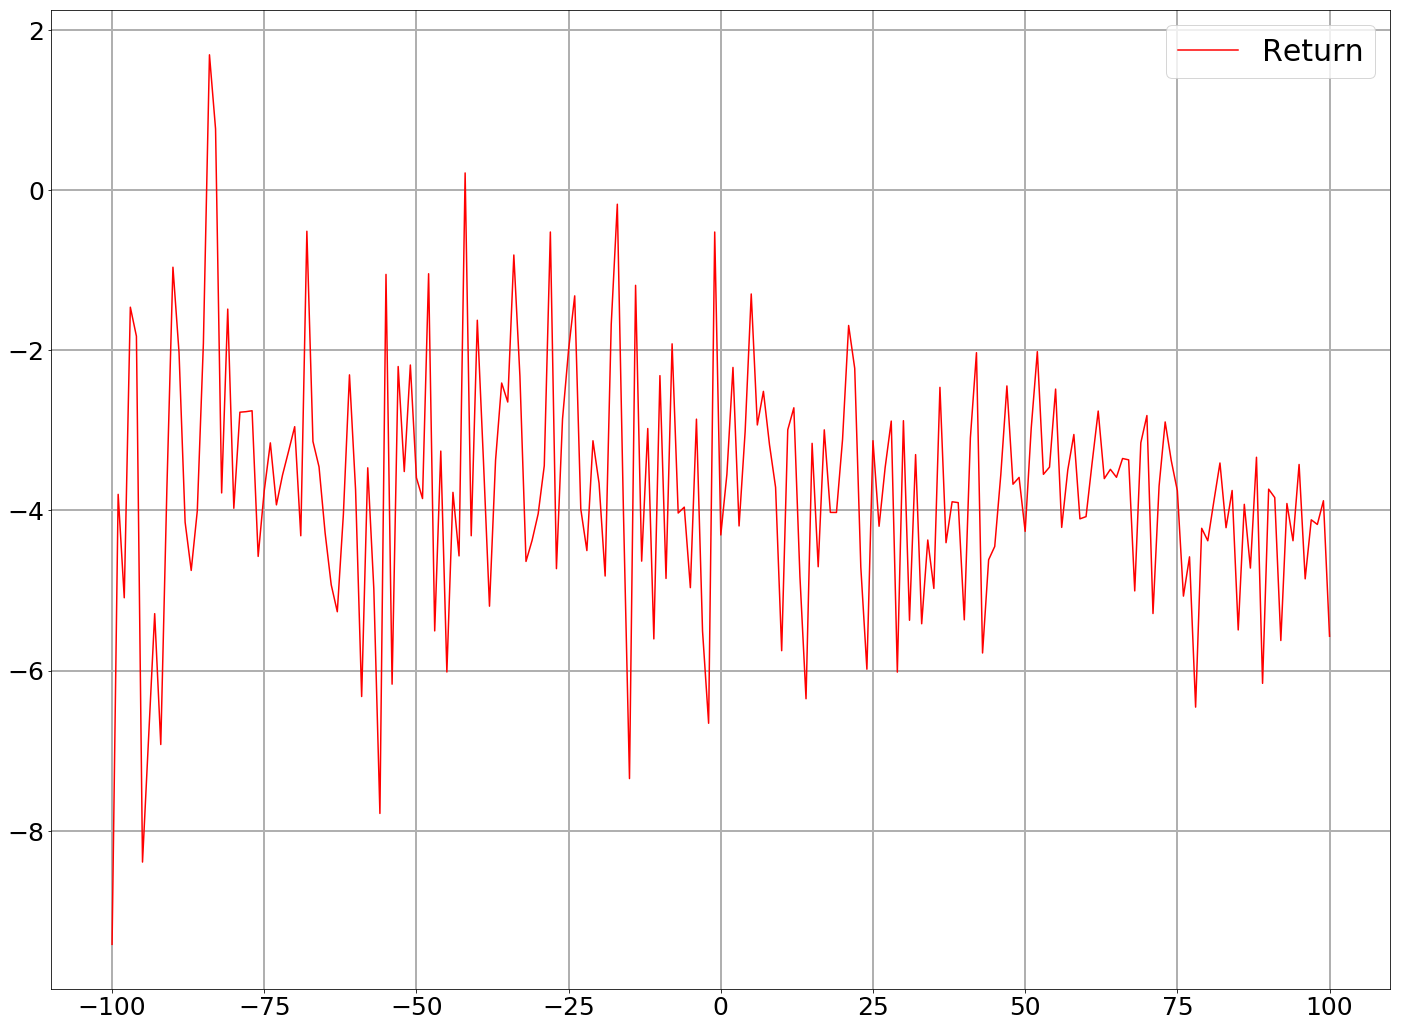
\includegraphics[width=\textwidth]{images/behaviour-up-60s-sell.png}
        \caption{Returns of sell orders 60 seconds}
        \label{fig:behvaiour-up-60s-sell}
    \end{subfigure}
    \begin{subfigure}[b]{0.45\textwidth}
        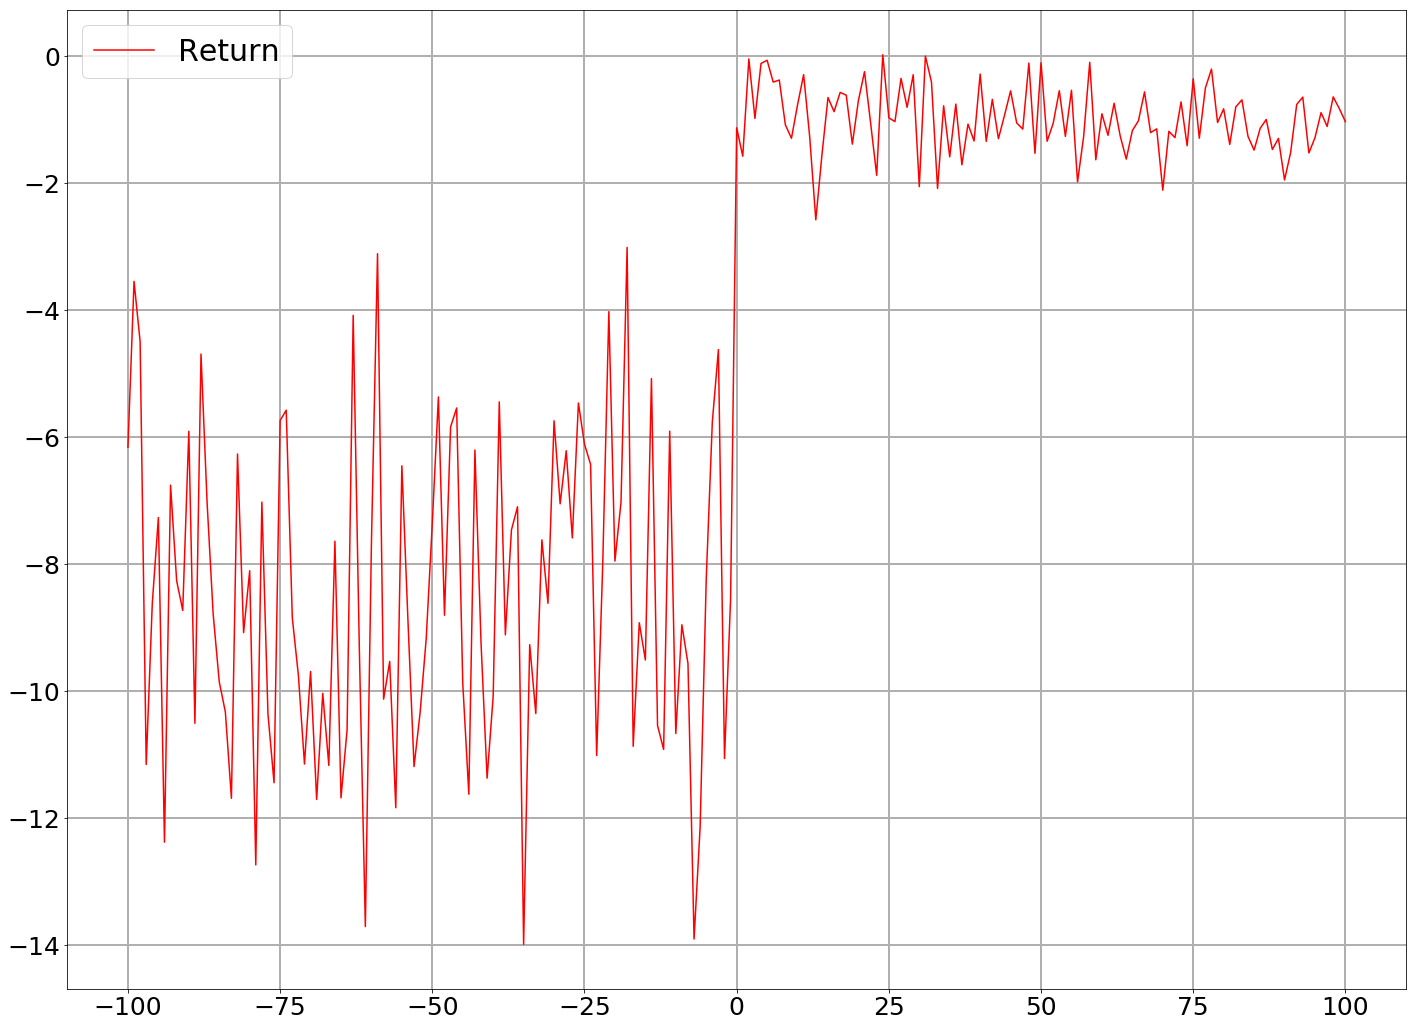
\includegraphics[width=\textwidth]{images/behaviour-up-100s-buy.png}
        \caption{Returns of buy orders 100 seconds}
        \label{fig:behvaiour-up-100s-buy}
    \end{subfigure}
    \begin{subfigure}[b]{0.45\textwidth}
        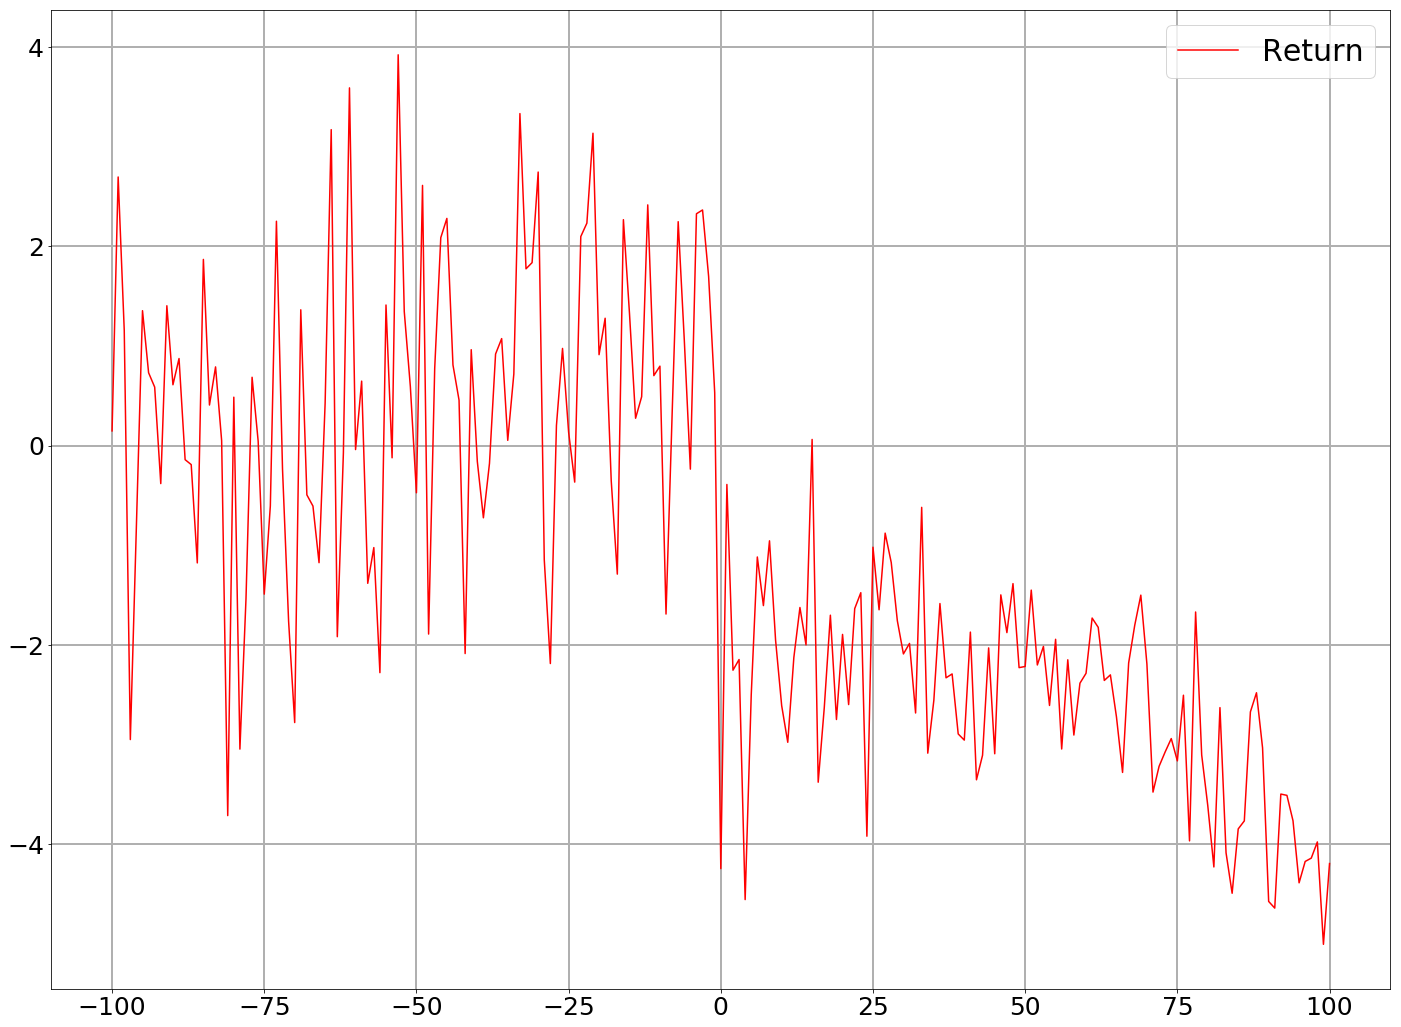
\includegraphics[width=\textwidth]{images/behaviour-up-100s-sell.png}
        \caption{Returns of sell orders 100 seconds}
        \label{fig:behvaiour-up-100s-sell}
    \end{subfigure}
    \caption{Returns of buy and sell orders executed within 10, 30, 60 and 100 seconds on data set II.}
    \label{fig:behvaiour-up}
\end{figure}

\subsection{Order placement behavior on data set II}
For data set II, which shows an upward price trend, the intuition is the opposite as for the investigation using data set I.
We expect buy orders to result in better returns when immediately filled, that is, when the agent crosses the spread and places the order high in the book ($a>0$).
The assumption is that, as time passes and the market price rises, other traders become less willing to sell at the market price or lower.
Therefore, the longer the time horizon given to the agent, the more critical it becomes to execute immediately;  otherwise, shares would have to be bought at an increased market price.
In contrast, better returns with sell orders are expected when placed deep in the book ($a<0$), meaning that they are sold at a higher price.
The assumption is that, as the price rises, market participants become more likely to buy assets at higher prices.
Hence, the longer the time horizon, the deeper in the book the agent should place a limit sell order.
We investigate these assumptions by performing the same experiment as in the previous section, with time horizons of 10, 30, 60 and 100 seconds, as shown in Figure \ref{fig:behvaiour-up}.

The returns of buy orders filled within a time horizon of 10 seconds, as shown in Figure \ref{fig:behvaiour-up-10s-buy}, correlate with the above-mentioned assumptions.
The highest returns are achieved when crossing the spread and, although limit levels in the range of 1-50 tend to perform the same, and considering the risk of paying a premium, the wisest choice for the agent would be to choose the level closest to the spread.
The sell orders placed with a time horizon of 10 seconds contradict the assumptions, as shown in Figure \ref{fig:behvaiour-up-10s-sell}.
The agent obtains the highest rewards when choosing a price for the order at market price $a=0$.
A highly negative limit level yields a return of  approximately \$3.00 less than when placing at the suggested market price.

With 30 seconds left to buy 1.0 BTC (Figure \ref{fig:behvaiour-up-30s-buy}), the orders placed with $a>0$ (above the spread) become stable for any such limit level.
This is likely due to the higher order pressure of data set II, as described in Section \ref{sec:analysis-data-sets}, as there are more market participants willing to sell.
The returns for limit sell orders, as shown in Figure \ref{fig:behvaiour-up-30s-sell}, become more rewarding as the agent benefits from a slight increase in price within the given time horizon.

This pattern becomes clearly apparent when a time horizon of 60 and 100 seconds was given, as shown in Figures \ref{fig:behvaiour-up-60s-sell} and \ref{fig:behvaiour-up-100s-sell} respectively.
With the increased time horizon, the assumptions stated in the beginning of this section are confirmed and the agent, when trying to sell shares, should indeed place orders deep in the order book ($a<0$).
As time passes and the market price rises, market participants are willing to buy at an increasing price and the agent is expected to be able to sell all assets at this increased price without the need for a further market order.
In contrast, if the agent decides to sell the assets at a decreasing price, as indicated by the higher limit levels, a lower reward can be expected when $a>0$.
More precisely, for a time horizon of 100 seconds, the agent is expected to receive up to \$7.00 less when choosing to cross the spread with a limit level of +100, as opposed to a negative limit level.
Figures \ref{fig:behvaiour-up-60s-buy} and \ref{fig:behvaiour-up-100s-buy} show the expected results of an agent that buys assets within 60 and 100 seconds respectively.
It is evident from the figures that the rise in the market price means that the expected damage can be minimized by crossing the spread and buying immediately.
The advice stated before remains valid: the agent should choose a price slightly above the market price as there is enough liquidity in the market to buy the demanded number of assets.

\subsection{Conclusion of empirical analysis}
From the results of the empirical analysis performed on data sets I and II, the following observations can be made with respect to limit order placement:
during a fall in the market price, the purchase prices of assets can be optimized by placing limit orders deep in the order book ($a<0$) and the least loss is sustained when selling assets immediately to the market price ($a>0$).
In contrast, during a rising market, it is suggested that assets be purchased using a market order ($a>0$) and sale prices can be optimized by placing the sell orders deep in the order book ($a<0$).
These effects become more apparent when a longer time horizon is given for an order. With regard to shorter time horizons, the order placement process tends to be either intercepted by short term fluctuations or low trading volumes.
The latter implies that, during an upwards trend, market participants are willing to buy and sell shares at higher prices and on the contrary, during a downwards trend at lower prices.
In this analysis, the orders placed had to be completely filled without the ability to take intermediate steps of canceling and replacing the order within the given time horizon.
Therefore, it falls to the reinforcement learners to evaluate whether or not such amendments to the order will result in a more favorable reward.
In order to have a measure of comparison for the reinforcement learning agents to come, Table \ref{tbl:analysis-empirical-summary} summarizes the findings and shows the expected rewards for (1) the optimal limit level chosen and (2) an immediate completion of the order using a market order.
\begin{table}[H]
\centering
\begin{tabular}{l|l|l|}
\cline{2-3}
& \textbf{$\mathbb{E}$[Limit order] (optimal)} & \textbf{\begin{tabular}[c]{@{}l@{}}$\mathbb{E}$[Market order]\end{tabular}} \\ \hline
\multicolumn{1}{|l|}{\textbf{Buy (I)}}   & 15.20          & -0.05                                                           \\ \hline
\multicolumn{1}{|l|}{\textbf{Sell (I)}}  & -27.70         & -27.70                                                          \\ \hline
\multicolumn{1}{|l|}{\textbf{Buy (II)}}  & -1.06          & -1.06                                                           \\ \hline
\multicolumn{1}{|l|}{\textbf{Sell (II)}} & 3.68          & -1.72                                                           \\ \hline
\multicolumn{1}{|l|}{\textbf{$\Sigma$}} & -9.88          & -30.53                                                           \\ \hline
\end{tabular}
\caption{Summary of rewards derived from the empirical analysis.}
\label{tbl:analysis-empirical-summary}
\end{table}

Furthermore, we ran the same experiment by using different action step parameters $\Delta{a}$, as shown in Table \ref{tbl:analysis-empirical-summary-a}.
Thereby, we found that a coarser step size does not improve the expected return for an optimal placed limit order.
As a result, we will henceforth use the setting $\Delta{a}=\$0.1$ for investigations undertaken with reinforcement learning agents.
\begin{table}[H]
\centering
\begin{tabular}{l|l|l|l|l|}
\cline{2-5} & \textbf{$\Delta{a}=\$0.1$} & \textbf{$\Delta{a}=\$0.2$} & \textbf{$\Delta{a}=\$0.5$} & \textbf{$\Delta{a}=\$1.0$} \\ \hline
\multicolumn{1}{|l|}{\textbf{\begin{tabular}[c]{@{}l@{}}$\mathbb{E}${[}Limit order{]} \\ (optimal)\end{tabular}}} & -9.88          & -9.96          & -13.52         & -17.65         \\ \hline
\end{tabular}
\caption{Rewards derived from the empirical analysis with different action step parameters $\Delta{a}$.}
\label{tbl:analysis-empirical-summary-a}
\end{table}

\section{Q-Learning without market variables}
\label{sec:eval-qlearn}
The previous section provided knowledge about the expected rewards an agent will receive when placing buy and sell orders using the reinforcement learning environment and with the underlying data set I and II.
For each such observation, a fixed time horizon was chosen for which an order was placed in the order book, followed by a market order in case the order has not been filled completely.

This section aims to investigate whether or not a Q-Learning agent, as described in Chapter \ref{chap:setup} (Section \ref{setup:q-learning}), can improve the rewards received over the expected return for a market order as derived in the previous section.
Thereby, the agent is allowed to cancel its order after every 10 seconds and place a new order with the remaining inventory (e.g. $\Delta{t}=10$), until the time horizon of 100 seconds has been fully consumed.
Subsequently, and in the event that the order has not been filled completely, a market order is issued for the remaining share to be bought or sold.
For both data sets (I and II), an independent learning experiment is being proceeded where the agent is supposed to either buy or sell shares.
In each experiment, the training is limited to 5000 epochs and 1000 orders are being placed and evaluated on the test set (defined as "backtesting").
The Q-Learning agent is set up as follows:
the learning rate selected $\alpha=0.1$ is small due to the extensive number of steps the agent will take throughout the epochs.
The discount factor $\gamma=0.5$ is chosen to balance the agent's incentive to profit from immediate rewards and consuming the entirety of the given time horizon.
Initially, the exploration constant $\epsilon$ is set to 0.8 and a decay is applied such that the factor reduces to $\epsilon=0.1$ by the time the training is completed.
This allows the agent first to explore the action space and then exploit on the learned optimal actions to take.

With this setup, four observations were made and for each, the training and testing results are stated below.
During training, the mean rewards and the average action chosen for each epoch were recorded.
Once the model was trained, a backtest was run on the test data sets, in which the agent executed orders by choosing from the learned optimal actions.

\subsection{Results of training and testing on data sets I and II}

\begin{figure}
    \centering
    \begin{subfigure}[b]{0.4\textwidth}
        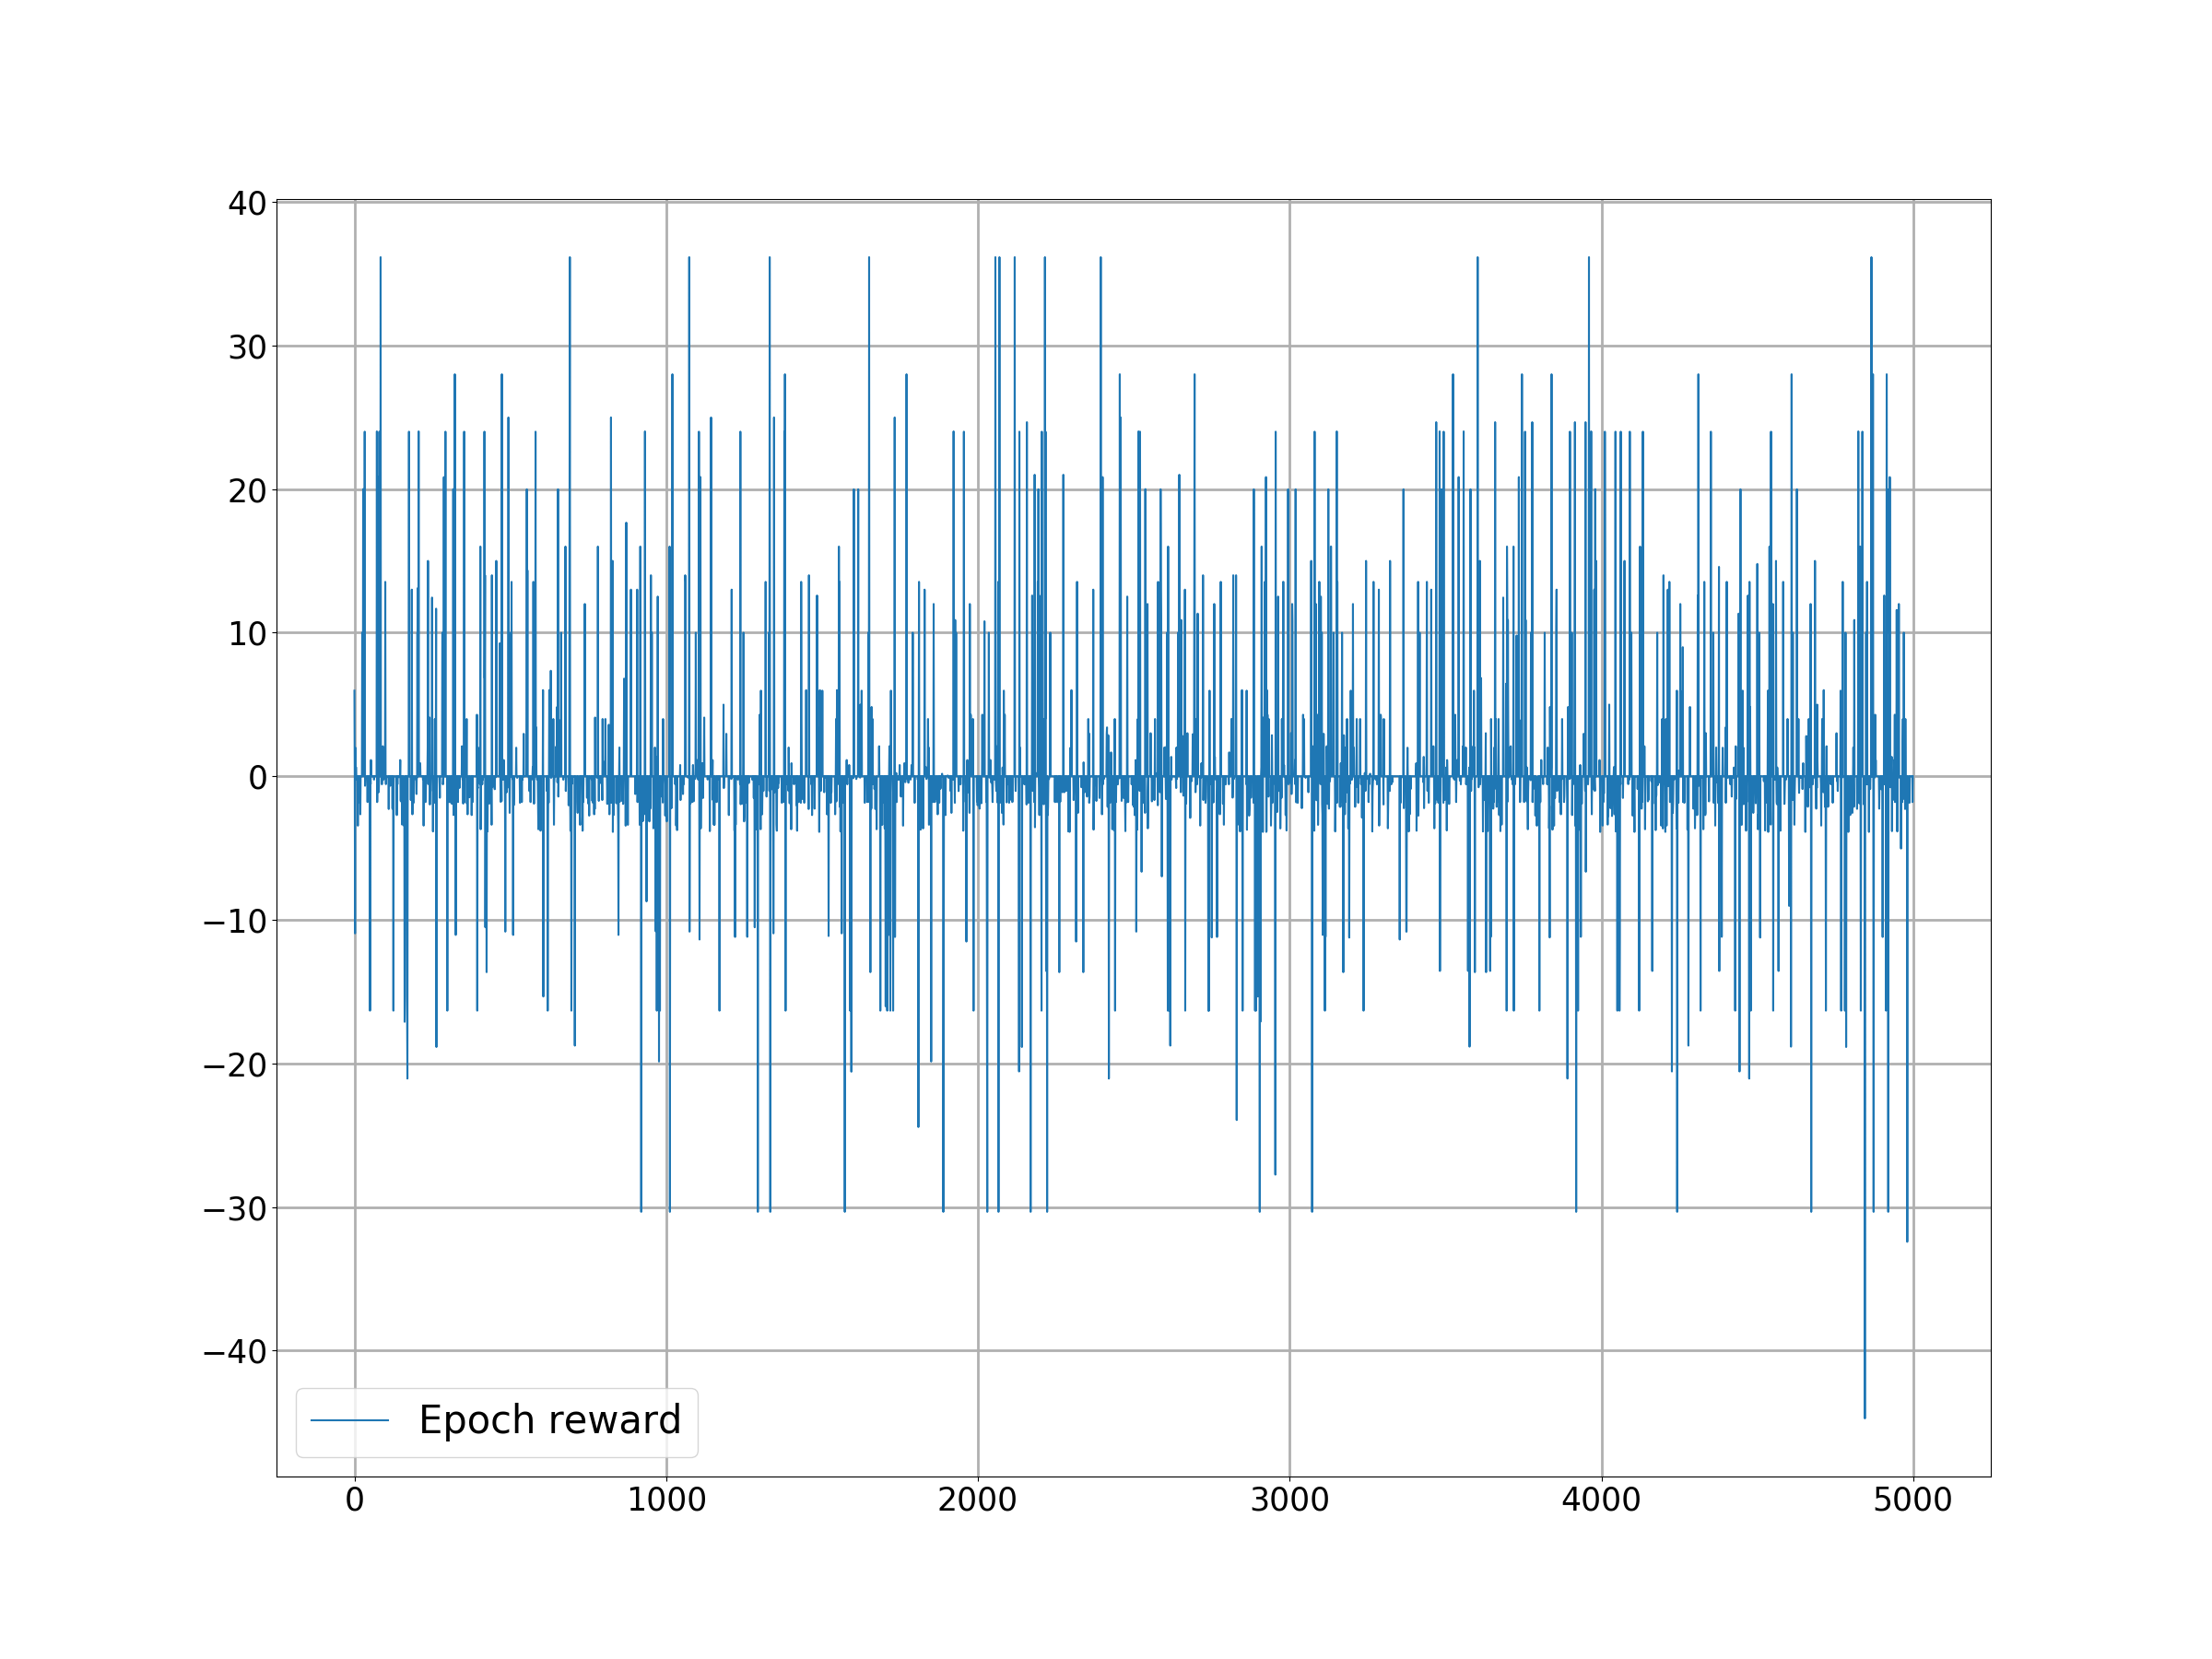
\includegraphics[width=\textwidth]{q_1_10000_BUY_rewards.png}
        \caption{Mean rewards per epoch (buy)}
        \label{fig:analysis-q-learn-1-reward-buy}
    \end{subfigure}
    \begin{subfigure}[b]{0.4\textwidth}
        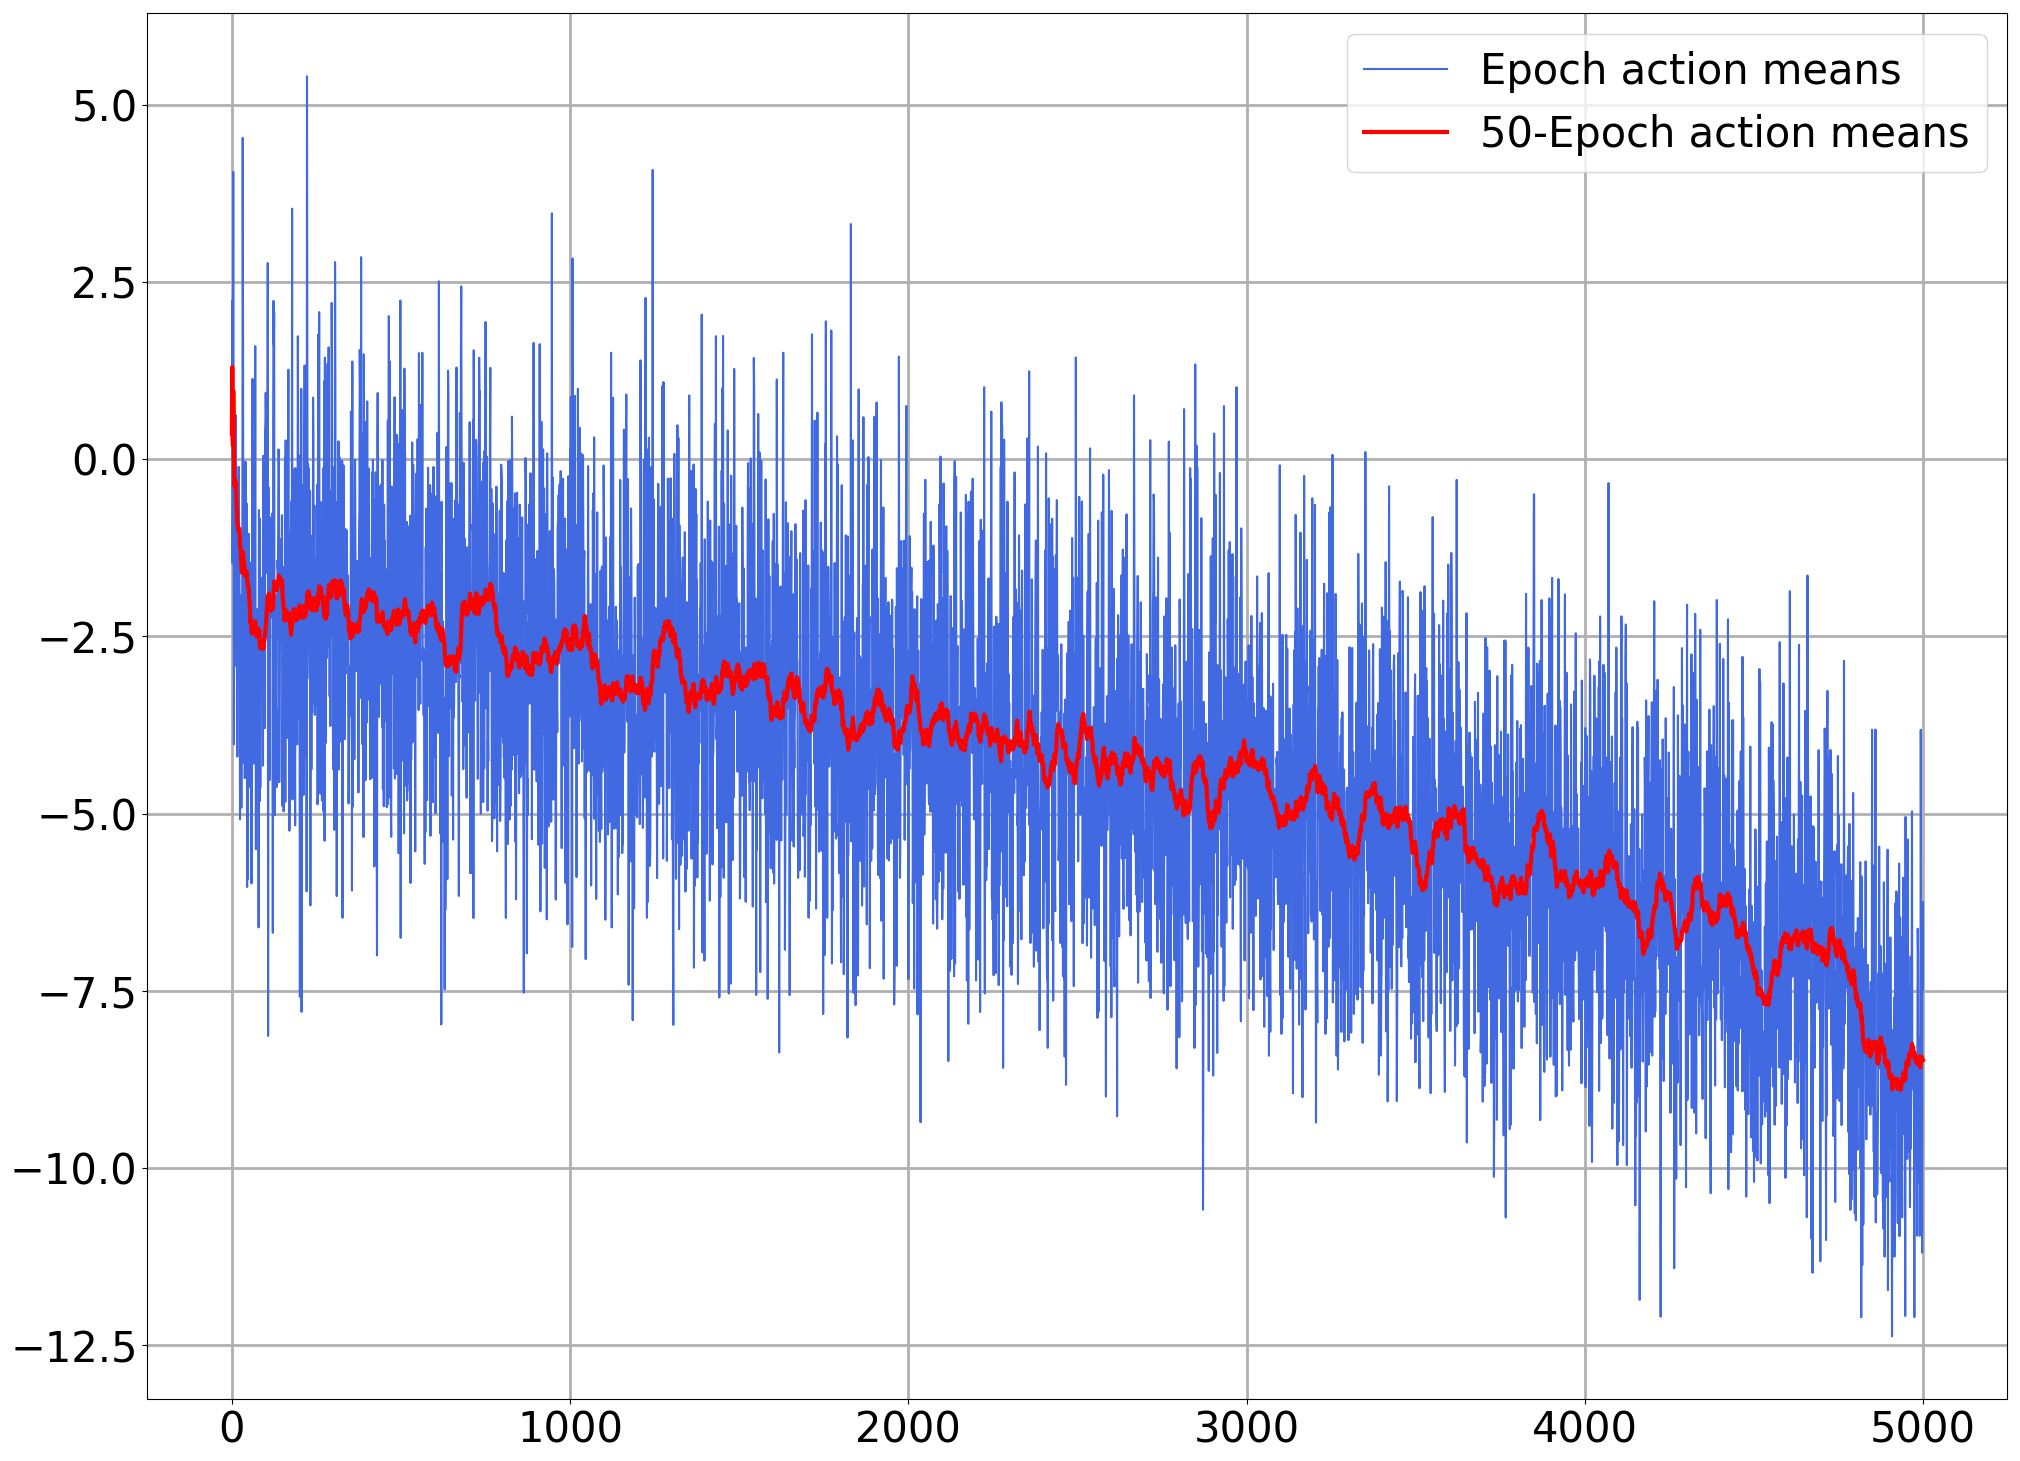
\includegraphics[width=\textwidth]{q_1_10000_BUY_mean_actions.png}
        \caption{Mean of actions per epoch (buy)}
        \label{fig:analysis-q-learn-1-action-buy}
    \end{subfigure}
    \begin{subfigure}[b]{0.4\textwidth}
        \includegraphics[width=\textwidth]{q_1_10000_SELL_rewards.png}
        \caption{Mean rewards per epoch (sell)}
        \label{fig:analysis-q-learn-1-reward-sell}
    \end{subfigure}
    \begin{subfigure}[b]{0.4\textwidth}
        \includegraphics[width=\textwidth]{q_1_10000_SELL_mean_actions.png}
        \caption{Mean of actions per epoch (sell)}
        \label{fig:analysis-q-learn-1-action-sell}
    \end{subfigure}
    \caption{Mean rewards and actions for buying and selling on training data set I.}
    \label{fig:analysis-q-learn-1}
\end{figure}
\begin{figure}
    \centering
    \begin{subfigure}[b]{0.4\textwidth}
        \includegraphics[width=\textwidth]{q_2_10000_BUY_rewards.png}
        \caption{Mean rewards per epoch (buy)}
        \label{fig:analysis-q-learn-2-reward-buy}
    \end{subfigure}
    \begin{subfigure}[b]{0.4\textwidth}
        \includegraphics[width=\textwidth]{q_2_10000_BUY_mean_actions.png}
        \caption{Mean of actions per epoch (buy)}
        \label{fig:analysis-q-learn-2-action-buy}
    \end{subfigure}
    \begin{subfigure}[b]{0.4\textwidth}
        \includegraphics[width=\textwidth]{q_2_10000_SELL_rewards.png}
        \caption{Mean rewards per epoch (sell)}
        \label{fig:analysis-q-learn-2-reward-sell}
    \end{subfigure}
    \begin{subfigure}[b]{0.4\textwidth}
        \includegraphics[width=\textwidth]{q_2_10000_SELL_mean_actions.png}
        \caption{Mean of actions per epoch (sell)}
        \label{fig:analysis-q-learn-2-action-sell}
    \end{subfigure}
    \caption{Mean rewards and actions for buying and selling on training data set II.}
    \label{fig:analysis-q-learn-2}
\end{figure}

Figure \ref{fig:analysis-q-learn-1} shows the training on data set I.
The average reward received during the training is shown in Figure \ref{fig:analysis-q-learn-1-reward-buy}.
Over the course of 5000 epochs, the agent was able to improve the mean reward by approximately $\sim$0.5, as a result of the change in actions chosen.  This is illustrated in Figure \ref{fig:analysis-q-learn-1-action-buy}.
The agent started off with the average action of $\sim$-3, which is a result of the low epsilon parameter that makes the agent choose actions randomly.
Actions were then adapted to the more negative side of the order book, such that after $\sim$1500 epochs, the agent chose actions as low as -20 and then adjusted and stagnated at $\sim$-15.
During the backtest, 1000 orders were executed on the test data set, which resulted in an average reward of \textit{-1.17}.
Making a comparison between the results of the empirical analysis performed on the same data set, as shown in Figure \ref{fig:behvaiour-down}, provides means for interpretation:
The policy learned by the Q-Learning agent performs worse than the expected cost of a market order, which was \$-1.12 when buying 1.0 BTC; this is shown in Section \ref{sec:eval-empirical}.
The highly negative average actions the agent choose toward the end of the training indicates that the order might not oftentimes have been able to be filled within the time horizon and an expensive market order had to follow.

The rewards received for the agents' tasks of selling the assets are much more volatile than for buying, as shown in Figure \ref{fig:analysis-q-learn-1-reward-sell}, and no clear improvement can be seen.
In addition, no significant adjustment was made by the agent regarding the mean of the actions chosen, as indicated in Figure \ref{fig:analysis-q-learn-1-action-sell}.
The backtest resulted in the achievement of an average reward of -21.34 by the agent.
The reward received for placing market orders on the test set account to a negative reward of -27.70.
Hence, the agent is able to save \$6.36 when selling 1.0 BTC.
\\
\\
Figure \ref{fig:analysis-q-learn-2} shows the experiment performed on data set II.
The average reward received while training to buy the asset is shown in Figure \ref{fig:analysis-q-learn-2-reward-buy}.
Throughout the epochs, the agent was able to improve the mean reward by approximately 0.5, which was a similar result to that obtained with the previous data set (I), .
Even though the trend of this data set is the opposite, the change in chosen actions correlates to the previous findings and is illustrated in Figure \ref{fig:analysis-q-learn-2-action-buy}.
The backtest on test data set II resulted in an average reward of \textit{-1.04} --,  again worse than the average reward received with the training set.
A market order on test data set to accounts to an average reward of -1.06, indicating that the agent's policy is saving \$0.02 when buying 1.0 BTC.
On the basis of the empirical analysis performed when buying on this data set, as shown in Figure \ref{fig:behvaiour-up}, and comparing it to the rewards received by the agent, implies that the agent failed to execute orders with the limit orders placed and oftentimes market orders must have followed.

As with the sell orders placed on data set I, the rewards received for the agent's tasks to sell the assets in data set II are very volatile, as shown in Figure \ref{fig:analysis-q-learn-1-reward-sell}.
No improvement can be seen from the rewards during the training and no significant adjustment was made by the agent regarding the actions chosen, as indicated in Figure \ref{fig:analysis-q-learn-2-action-sell}.
The backtest resulted in an average reward of -4.74 achieved by the agent, whereas market orders are expected to result in an average reward of -1.72.
Hence, the use of an requires the payment of a premium of \$3.02 when selling 1.0 BTC.

\subsection{Conclusion of Q-Learning approach}

\begin{table}[H]
\centering
\begin{tabular}{l|l|l|}
\cline{2-3}
& \textbf{Q-Learner} & \textbf{\begin{tabular}[c]{@{}l@{}}$\mathbb{E}$[Market\\ Order]\end{tabular}} \\ \hline
\multicolumn{1}{|l|}{\textbf{Buy (I)}}   & -1.17          & -0.05                                                           \\ \hline
\multicolumn{1}{|l|}{\textbf{Sell (I)}}  & -21.34         & -27.70                                                          \\ \hline
\multicolumn{1}{|l|}{\textbf{Buy (II)}}  & -1.04          & -1.06                                                           \\ \hline
\multicolumn{1}{|l|}{\textbf{Sell (II)}} & -4.74          & -1.72                                                           \\ \hline
\multicolumn{1}{|l|}{\textbf{$\Sigma$}} & -28.29          & -30.53                                                           \\ \hline
\end{tabular}
\caption{Summary of rewards for the Q-Learning agent and market orders.}
\label{tbl:analysis-q-learn-summary}
\end{table}
The findings of this section are summarized in Table \ref{tbl:analysis-q-learn-summary}.
We conclude that the Q-Learning agent was not able to constantly place buy and sell orders in a way which would result in a price better than the current market price.
Oftentimes, a market order, which would trigger an immediate purchase or sale, would be the better choice.
Clearly, this is due to the fact that the agent was not able to find the most suitable actions.
Furthermore, in order to investigate whether or not these findings were a result of the agent aiming for a reward that was too immediate, the same experiment was performed with $\gamma=0.3$ and therefore rely more extensively on the future rewards.
However, no improvement could be achieved and instead, the agent achieved similar rewards while requiring more epochs in order to converge to the same mean of actions.
In this section, we have only investigated the mean of the actions chosen throughout an epoch, which has provided evidence, which we regard as sufficient, that the chosen actions resulted mostly in market orders.
Furthermore, it is to be assumed that the absence of market variables, while only relying on the given rewards, makes it hard for any learner to determine an optimal policy.
Therefore, the following section will make use of market variables in order to determine whether or not a learner can exploit the information hidden in the market and therefore act in favor of optimally placing limit orders.

\section{Deep Q-Network with market features}
\label{sec:eval-dqn}
In the previous section, the Q-Learning agent was trained on data sets I and II, and no significant optimization in terms of the buying and selling of assets was achieved.
By considering the above-mentioned results of the empirical analysis of the limit order placement behavior, we found that most of the limit orders placed by the Q-Learning agent were not filled within the given time horizon and instead, market orders had to be submitted after the time was consumed.

In this section, we aim to determine whether or not the DQN agent is capable of extracting information provided by the raw market features and therefore improve the limit order placement policy.
The setup is the same as in the previous section, where the agents task is to buy and sell 1.0 BTC within 100 seconds with discrete step size $\Delta{t}=10$ in both data sets I and II.
Furthermore, both of the features constructed in Chapter \ref{chap:data}, will be applied and investigated separately.
The input shape of the model in use that approximates the action-value function, as described in Chapter \ref{chap:preliminaries} (Section \ref{sec:deep-reinforcement-learning}), is determined by the feature in use and is described below.
We evaluate the performance of the DQN agent under the application of both neural network architectures, the standard convolutional neural network and the multilayer perceptron, as presented in Section \ref{setup:dqn}.
For both of these DQN agent setups, we rely on the default hyperparameters worked out by Mnih et al. \cite{mnih2015human}, as shown in Figure \ref{fig:eval-dqn-hyperparameters}.
Furthermore, we will train both agents with 5000 epochs and will test with 1000 epochs.
Finally, we will conclude our findings and determine the capabilities of the DQN approach (and its use of the market features) by comparing it to the expected returns for a market order calculated earlier in Section \ref{sec:eval-empirical}.
\begin{figure}[H]
    \centering
    \makebox[\linewidth]{
        \includegraphics[width=14cm]{images/dqn_hyperparameters.png}
    }
    \caption{The values of all the hyperparameters were selected. We did not perform a systematic grid search owing to the high computational cost, although it is conceivable that better results could be obtained by tuning these hyperparameter values.}
    \label{fig:eval-dqn-hyperparameters}
\end{figure}

\subsection{Application of historical order feature}

The following evaluation of the DQN agent setups that consider Feature I, as described in Chapter \ref{chap:data} (Section \ref{sec:data-feature-1}).
Furthermore, in this initial run we consider $m=30$ historical order book states, alongside the maximum number of bid and ask levels $n=40$.
This results in a feature set size of $(60, 40, 2)$, as a consequence of the defined size $(2*m, n, 2)$.
When we included the two private variables by appending a vector $[inventory, time]$ at the beginning of this feature vector, the size of the feature set was $(61, 40, 2)$ and, as such, will serve as the input for the neural networks in use.

\begin{figure}[H]
    \centering
    \begin{subfigure}[b]{0.4\textwidth}
        \includegraphics[width=\textwidth]{cnn_nn_1_buy_bidask_rewards.png}
        \caption{Reward per epoch (buy)}
        \label{fig:analysis-dqn-1-reward-buy}
    \end{subfigure}
    \begin{subfigure}[b]{0.4\textwidth}
        \includegraphics[width=\textwidth]{cnn_nn_1_buy_bidask_mean_actions.png}
        \caption{Mean of actions per epoch (buy)}
        \label{fig:analysis-dqn-1-action-buy}
    \end{subfigure}
    \begin{subfigure}[b]{0.4\textwidth}
        \includegraphics[width=\textwidth]{cnn_nn_1_sell_bidask_rewards.png}
        \caption{Mean rewards per epoch (sell)}
        \label{fig:analysis-dqn-1-reward-sell}
    \end{subfigure}
    \begin{subfigure}[b]{0.4\textwidth}
        \includegraphics[width=\textwidth]{cnn_nn_1_sell_bidask_mean_actions.png}
        \caption{Mean of actions per epoch (sell)}
        \label{fig:analysis-dqn-1-action-sell}
    \end{subfigure}
    \caption{DQN agent rewards and mean of actions for buying and selling on training data set I using feature I.}
    \label{fig:analysis-dqn-1}
\end{figure}

\begin{figure}[H]
    \centering
    \begin{subfigure}[b]{0.4\textwidth}
        \includegraphics[width=\textwidth]{cnn_nn_2_buy_bidask_rewards.png}
        \caption{Reward per epoch (buy)}
        \label{fig:analysis-dqn-2-reward-buy}
    \end{subfigure}
    \begin{subfigure}[b]{0.4\textwidth}
        \includegraphics[width=\textwidth]{cnn_nn_2_buy_bidask_mean_actions.png}
        \caption{Mean of actions per epoch (buy)}
        \label{fig:analysis-dqn-2-action-buy}
    \end{subfigure}
    \begin{subfigure}[b]{0.4\textwidth}
        \includegraphics[width=\textwidth]{cnn_nn_2_sell_bidask_rewards.png}
        \caption{Mean rewards per epoch (sell)}
        \label{fig:analysis-dqn-2-reward-sell}
    \end{subfigure}
    \begin{subfigure}[b]{0.4\textwidth}
        \includegraphics[width=\textwidth]{cnn_nn_2_sell_bidask_mean_actions.png}
        \caption{Mean of actions per epoch (sell)}
        \label{fig:analysis-dqn-2-action-sell}
    \end{subfigure}
    \caption{DQN agent rewards and mean of actions for buying and selling on training data set II using feature I.}
    \label{fig:analysis-dqn-2}
\end{figure}

Figure \ref{fig:analysis-dqn-1} shows the learning process using data set I.
During the training process relating to the purchase of assets, the rewards obtained consistently improved over the course of the 5000 epochs (Figure \ref{fig:analysis-dqn-1-reward-buy}), throughout which the DQN-CNN agent steadily adjusted its actions to be more negative and the DQN-MLP agent adjusted them to become more positive (Figure \ref{fig:analysis-dqn-1-action-buy}).
It is evident that this adjustment, for both DQN agents, is not as linear as it was during the training of the Q-Learning agent, as shown in the previous section.
However, the adjustment made by the DQN-CNN agent is appropriate since the market price was falling.
The rewards obtained from selling are shown in Figure \ref{fig:analysis-dqn-1-reward-sell} and the average chosen action throughout the epochs is shown in Figure \ref{fig:analysis-dqn-1-action-sell}.
The rewards did not improve over the course of the training and both agents did not choose to adjust the average actions.
Possibly, this was due to the constantly negative rewards obtained during the training under market conditions that were difficult for the sale of assets while the market price was falling.
Figure \ref{fig:analysis-dqn-2} shows the agents learning processes using data set II.
Over the course of 5000 epochs, the agents were not able to improve their reward and instead, stagnated at approximately \$-2.50 and \$5.00 rewards per epoch respectively, as shown in Figure \ref{fig:analysis-dqn-2-reward-buy}.
Both agents adjusted the actions steadily such that the average limit level fell to approximately -20 at epoch 1000 and remained at this level, as shown in Figure \ref{fig:analysis-dqn-2-action-buy}.
Therefore, the rewards must have been determined by market orders followed after those which failed to fill the order with their levels chosen.
The rewards for the agent that learned to sell assets are shown in Figure \ref{fig:analysis-q-learn-2-reward-sell}.
The rewards could not be improved during the training, even though the agent lowered the average action chosen to below -20, as shown in Figure \ref{fig:analysis-q-learn-2-action-sell}.
In such rising market conditions, the rewards observed are a product of the market order, since negative actions will likely not result in a filled order.
The rewards for selling assets in this rising market was improved and remained above \$0.00, as shown in Figure \ref{fig:analysis-q-learn-2-reward-sell}.
Thereby, the average of the actions chosen for an epoch reduced within the first 1000 epochs and, thereafter, remained at approximately -10 (DQN-CNN) and -20 (DQN-MLP), which correlates with the rewards obtained .
\\
\\
Table \ref{tbl:analysis-dqn-orderfeature-summary} summarizes the average rewards observed during the backtest using the DQN agents that made use of Feature I.
Overall, both DQN agents were able to optimize limit order placement when the given market conditions became favorable to making a purchase or sale respectively.
More precisely, significant improvements were made during the backtest of the DQN-CNN agent when the task was to buy assets and the market price was falling (data set I). 
Thereby, the agent was rewarded with 22.06, which is a significant improvement compared to the expected return of -0.05 for a market order.
Likewise, during rising market conditions (data set I), both agents were able to improve by more than the expected market order return.
However, when market conditions were not favorable to an intention to either buy or sell, the agents mostly performed not only worse than the expected return of a market order but also worse than the Q-Learning agent (see Table \ref{tbl:analysis-q-learn-summary} above).
That is, the DQN-CNN agent achieved rewards of -39.26 and -2.26 when selling in data set I and buying in data set II, which were both worse than the expected returns for market orders.
The exception was when the DQN-MLP agent achieved -22.67 when attempting to make sales in data set I and therefore, it performed better than the expected market order return.
However, the backtest that set the DQN-MLP agent to make purchases in data set II performed, with -7.40, much worse than the baseline provided by the expected market order return.
Overall, the DQN-CNN agent performed the best and minor improvements were achieved by the DQN-MLP agent.

\begin{table}[H]
\centering
\begin{tabular}{l|l|l|l|}
\cline{2-4}
& \textbf{DQN-CNN} & \textbf{DQN-MLP} & \textbf{\begin{tabular}[c]{@{}l@{}}$\mathbb{E}$[Market\\ Order]\end{tabular}} \\ \hline
\multicolumn{1}{|l|}{\textbf{Buy (I)}}   & 22.06  & -4.04 & -0.05                                                           \\ \hline
\multicolumn{1}{|l|}{\textbf{Sell (I)}}  & -39.26 & -22.67        & -27.70                                                          \\ \hline
\multicolumn{1}{|l|}{\textbf{Buy (II)}}  & -2.26  & -7.40        & -1.06                                                           \\ \hline
\multicolumn{1}{|l|}{\textbf{Sell (II)}} & 0.84   & 7.47       & -1.72                                                           \\ \hline
\multicolumn{1}{|l|}{\textbf{$\Sigma$}} & -18.62  & -26.64        & -30.53                                                           \\ \hline
\end{tabular}
\caption{Summary of rewards during backtest of DQN agent using Feature I (historical orders).}
\label{tbl:analysis-dqn-orderfeature-summary}
\end{table}

\subsection{Application of historical trade feature}

The following evaluation of the DQN agent setups that consider Feature II, as described in Chapter \ref{chap:data} (Section \ref{sec:data-feature-2}).
In this initial run we consider $n=30$ historical trades.
This results in a feature set size of $(30, 3)$, as a consequence of the defined size $(n, 4)$.
When we included the two private variables by appending a vector $[inventory, time, 0, 0]$ at the beginning of this feature vector, the size of the feature set was $(31, 4)$ and, as such, will serve as the input for the neural networks in use.

\begin{figure}[H]
    \centering
    \begin{subfigure}[b]{0.4\textwidth}
        \includegraphics[width=\textwidth]{cnn_nn_1_buy_trades_rewards.png}
        \caption{Reward per epoch (buy)}
        \label{fig:analysis-dqn-1-trades-reward-buy}
    \end{subfigure}
    \begin{subfigure}[b]{0.4\textwidth}
        \includegraphics[width=\textwidth]{cnn_nn_1_buy_trades_mean_actions.png}
        \caption{Mean of actions per epoch (buy)}
        \label{fig:analysis-dqn-1-trades-action-buy}
    \end{subfigure}
    \begin{subfigure}[b]{0.4\textwidth}
        \includegraphics[width=\textwidth]{cnn_nn_1_sell_trades_rewards.png}
        \caption{Mean rewards per epoch (sell)}
        \label{fig:analysis-dqn-1-trades-reward-sell}
    \end{subfigure}
    \begin{subfigure}[b]{0.4\textwidth}
        \includegraphics[width=\textwidth]{cnn_nn_1_sell_trades_mean_actions.png}
        \caption{Mean of actions per epoch (sell)}
        \label{fig:analysis-dqn-1-trades-action-sell}
    \end{subfigure}
    \caption{DQN agent rewards and mean of actions for buying and selling on training data set I using feature II.}
    \label{fig:analysis-dqn-1-trades}
\end{figure}

\begin{figure}[H]
    \centering
    \begin{subfigure}[b]{0.4\textwidth}
        \includegraphics[width=\textwidth]{cnn_nn_2_buy_trades_rewards.png}
        \caption{Reward per epoch (buy)}
        \label{fig:analysis-dqn-2-trades-reward-buy}
    \end{subfigure}
    \begin{subfigure}[b]{0.4\textwidth}
        \includegraphics[width=\textwidth]{cnn_nn_2_buy_trades_mean_actions.png}
        \caption{Mean of actions per epoch (buy)}
        \label{fig:analysis-dqn-2-trades-action-buy}
    \end{subfigure}
    \begin{subfigure}[b]{0.4\textwidth}
        \includegraphics[width=\textwidth]{cnn_nn_2_sell_trades_rewards.png}
        \caption{Mean rewards per epoch (sell)}
        \label{fig:analysis-dqn-2-trades-reward-sell}
    \end{subfigure}
    \begin{subfigure}[b]{0.4\textwidth}
        \includegraphics[width=\textwidth]{cnn_nn_2_sell_trades_mean_actions.png}
        \caption{Mean of actions per epoch (sell)}
        \label{fig:analysis-dqn-2-trades-action-sell}
    \end{subfigure}
    \caption{DQN agent rewards and mean of actions for buying and selling on training data set II using feature II.}
    \label{fig:analysis-dqn-2-trades}
\end{figure}

Figure \ref{fig:analysis-dqn-1-trades} illustrates the learning processes of the DQN agents when buying and selling in data set I.
As with the agents that were provided by Feature I, the rewards received when buying slightly improved over the course of the 5000 epochs, which is shown in Figure \ref{fig:analysis-dqn-1-trades-reward-buy}.
Interestingly, the average action chosen per epoch by the DQN-CNN agent was abruptly adjusted after 4000 epochs, while the DQN-MLP's choice remained between 0 and 20, on average.
However, correlating improvements with respect to the rewards were not evident.
The rewards received when selling remained just below -10 for the DQN-CNN agent and below -20 for the DQN-MLP agent, as shown in Figure \ref{fig:analysis-dqn-1-trades-reward-sell}.
The average of the actions chosen by the DQN-CNN agent, though volatile, were adjusted towards becoming positive, as shown in Figure \ref{fig:analysis-dqn-1-trades-action-sell}.
Unfortunately, this is evidence that the average action does not provide enough insights into the actual decision-making process of the agent.
Had the agent consistently chosen positive actions throughout an epoch, an improvement in the reward would have been visible in the aforementioned figure.
Instead, the agent must have chosen negative actions in the initial steps and shifted towards very positive actions later in the epoch.
Figure \ref{fig:analysis-dqn-2-trades} illustrates the same learning process with the application of data set II.
The rewards for the buying process were not improved (Figure \ref{fig:analysis-dqn-2-trades-reward-buy}) for either of the two agents.
Interestingly, in this scenario, the DQN-MLP made a significantly better adjustment regarding the actions chosen (Figure \ref{fig:analysis-dqn-2-trades-action-buy}), indicating its willingness to make more immediate purchases.
Rewards for selling in data set II increased during the training, as shown in Figure \ref{fig:analysis-dqn-2-trades-reward-sell} and the average action chosen remained at around -30 after 1000 epochs, for both agents, as shown in Figure \ref{fig:analysis-dqn-2-trades-action-sell}.
\\
\\
Table \ref{tbl:analysis-dqn-tradefeature-summary} summarizes the average rewards received by the DQN agents during the backtest.
As with the previous application of Feature I to the DQN agents, significant optimization could be achieved when market conditions became more favorable to buying or selling.
For buying during falling market conditions (data set I), the DQN-CNN achieved a reward of 31.92 and the DQN-MLP a reward of 25.44, clear improvements compared to the expected market order return of -0.05.
Likewise, both agents improved sales in data set II (0.15 and 3.80 reward respectively).
Compared to when Feature I was applied, the agents under the application of Feature II achieved better results in difficult market conditions (selling in data set I and buying in data set II).
Particularly, sales in data set II were better than the expected returns of market orders.
Overall, as indicated by the positive sum of rewards achieved, both DQN agents were able to make purchases and sales of better than the market price.
Consequently, the rewards obtained were much better than the expected market order return.
The application of Feature II meant that the agent outperformed the DQN agent with Feature I (see Table \ref{tbl:analysis-dqn-orderfeature-summary} for comparison).
Thereby, it is evident that the DQN-CNN setup has yielded greater improvements than the DQN-MLP setup.

\begin{table}[H]
\centering
\begin{tabular}{l|l|l|l|}
\cline{2-4}
& \textbf{DQN-CNN} & \textbf{DQN-MLP} & \textbf{\begin{tabular}[c]{@{}l@{}}$\mathbb{E}$[Market\\ Order]\end{tabular}} \\ \hline
\multicolumn{1}{|l|}{\textbf{Buy (I)}}   & 31.92    & 25.44          & -0.05                                                           \\ \hline
\multicolumn{1}{|l|}{\textbf{Sell (I)}}  & -25.15   & -20.65         & -27.70                                                          \\ \hline
\multicolumn{1}{|l|}{\textbf{Buy (II)}}  & -3.56    & -6.43          & -1.06                                                           \\ \hline
\multicolumn{1}{|l|}{\textbf{Sell (II)}} & 0.15     & 3.80          & -1.72                                                           \\ \hline
\multicolumn{1}{|l|}{\textbf{$\Sigma$}} & 3.36      & 2.16          & -30.53                                                           \\ \hline
\end{tabular}
\caption{Summary of rewards during backtest of DQN agent using Feature II (historical trades).}
\label{tbl:analysis-dqn-tradefeature-summary}
\end{table}

\subsection{Comparison with different feature sizes}
\label{subsec:eval-comparison-feature-size}

Both features constructed in this project allow for size-related adjustments that determine the information content provided to the agent.
Until now, we have made use of one particular setting for each feature, that is, we have used $m_I=30$ windows with length $n_I=40$ for feature I and a vector length of $n_{II}=30$ for feature II.
With the use of the DQN-CNN agent, which has resulted in slightly better performance than the DQN-MLP agent, we will investigate whether or not a different size of the feature vector improve these results further.
We will proceed with the same evaluation as described in the previous two sections, but with different feature vector settings.
For feature I, we will investigate window sizes $m=10,20,30,40,50$ with maximum vector length $n=40$.
Similarly, for feature II, we will investigate the length of the vector $n=10,20,30,40,50$ (no window present for this feature).

Table \ref{tbl:analysis-dqn-featuresize} below shows the results from the backtest and confirms that the setting we ran earlier in this section performed the best.
It is evident that a smaller window size for feature I and a smaller vector length for feature II ($m_I<30$ and $n_{II}<30$) both have a negative impact on the resulting performance, indicating that the agent retrieved insufficient information.
However, increasing the dimensionality of our feature space ($m_I>30$ and $n_{II}>30$) did not improve the agents' capabilities and therefore indicates difficulties arising from the curse of dimensionality\cite{keogh2011curse}.

\begin{table}[H]
\centering
\begin{tabular}{|c|l|l|}
\hline
\textbf{\#}  & \multicolumn{1}{c|}{\textbf{\begin{tabular}[c]{@{}c@{}}Feature I\\ $\Sigma{[B1,S1,B2,BS2]}$\end{tabular}}} & \multicolumn{1}{c|}{\textbf{\begin{tabular}[c]{@{}c@{}}Feature II\\ $\Sigma{[B1,S1,B2,BS2]}$\end{tabular}}} \\ \hline
\textbf{10} & -36.85                                                                                                & -12.36                                                                                                 \\ \hline
\textbf{20} & -34.62                                                                                                & -13.68                                                                                                 \\ \hline
\textbf{30} & {\ul -18.62}                                                                                          & {\ul 3.36}                                                                                             \\ \hline
\textbf{40} & -21.59                                                                                                & -11.97                                                                                                 \\ \hline
\textbf{50} & -23.37                                                                                                & -1.43                                                                                                  \\ \hline
\end{tabular}
\caption{Summary of rewards during backtest of DQN-CNN agent using different feature sizes.}
\label{tbl:analysis-dqn-featuresize}
\end{table}

\section{Determining the limitations of the DQN agent}
\label{sec:eval-dqn-limitations}
This section aims to determine the capabilities and limitations of the DQN agent with the use of Feature I in greater detail.
Sample order submissions are investigated which uncover the actions chosen by an agent throughout one epoch.
Therefore, we will be able to see which market situations prevented the agent from achieving a positive reward and conclude why the agent was not able to choose the most appropriate actions.
In addition, artificial order books are being created which serve as new data sets to train and test the DQN agent on.
With their aid, we aim to determine the capabilities of the deep reinforcement learning technique under market conditions which are 1) not affected by short-term fluctuations and 2) a hold constant spread between best bid and best ask is given.

\subsection{Limitation arising from market situations or inappropriate actions from the agent}
Extensive investigations have shown that the DQN agent fails to place orders that lead to constant positive rewards for the following two reasons: 1) when the market situation does not allow the agent to do so and 2) when the agent submits an inappropriate action.

Our investigations have shown that, for the first category, it is not just upwards and downwards trends which make it difficult for the order placement to result in a positive reward, but also when the spread between the best bid and best ask price becomes large.
Examples of wide spread scenarios are shown in Figures \ref{fig:analysis-limit-wide-spread-buy} and \ref{fig:analysis-limit-wide-spread-sell}, where an agent attempted the placement of a buy and sell order respectively.
\begin{figure}[H]
    \centering
    \makebox[\linewidth]{
        \includegraphics[width=\textwidth]{images/analysis-limit-wide-spread-buy}
    }
    \caption{Wide spread between bid and ask prevents agent from buying.}
    \label{fig:analysis-limit-wide-spread-buy}
\end{figure}
\begin{figure}[H]
    \centering
    \makebox[\linewidth]{
        \includegraphics[width=\textwidth]{images/analysis-limit-wide-spread-sell}
    }
    \caption{Wide spread between bid and ask prevents agent from selling.}
    \label{fig:analysis-limit-wide-spread-sell}
\end{figure}
Prior to the start of the buy order placement, the spread between the best bid and best ask price was very close, as indicated by the green and red lines.
However, during the placement of this order, the spread widened and remained larger than \$50.00 for almost the entire time horizon.
Since the actions are segmented into discrete steps of $\Delta{a}=0.10$, with a total of 101 steps, and a market price ranging from -\$5.00 to +\$5.00, the agent had no chance of placing the orders close to the best ask price.
As a result, the entire inventory of 1.0 BTC bought by using a market order at the end of the time horizon (a trade is marked with a cross).
This generated a negative reward of -8.08.
The same market situation is demonstrated during which the agent initiated the process of placing a sell order.
Similarly, the pricing level was close to the best bid price only once.
As a result, a market order followed in which the agent sold the remaining 0.9 BTC at a decreased price that resulted in a negative reward of -47.28.
In addition, since there was not much liquidity offered by buyers, the market order was partially filled at decreasing price levels, as indicated by the crosses in the figure.
Two possible ways to overcome this limitation would be to either increase the number of steps or to increase the action step size; both approaches will be addressed in Chapter \ref{chap:discussion}.
\begin{figure}[H]
    \centering
    \makebox[\linewidth]{
        \includegraphics[width=10cm]{images/analysis-limit-impatient}
    }
    \caption{Wide spread between bid and ask prevents agent from selling.}
    \label{fig:analysis-limit-impatient}
\end{figure}
An example of the second category, where the agent clearly failed to select an appropriate action, is shown in Figure \ref{fig:analysis-limit-impatient}.
As is illustrated, the market price, and the best bid and ask price were declining before the initialization of the sell order placement. 
The agent then decided to cross the spread in the first step and choose action 28, which meant that it was willing to sell for \$2.80 below the market price.
By doing this, the order was immediately filled and resulted in a negative reward of -1.71.
Ideally, the agent should have been more patient and decided to place a limit order below the spread.
Then, in a subsequent step, the order could have been filled by means of a negative action, which would have resulted in a positive reward.
It is assumed that the agent failed to generalize the development of the order book with the provided feature set.
Instead, the agent reacted to the previous, declining market situation, in which  the better choice would certainly have been to immediately fill the sell order.

\subsection{Capabilities evaluated using artificial limit order books}

Introducing an artificially created order book allows us to determine the capabilities of a reinforcement learning agent in greater detail.
We define the formation of the order book states over time and therefore can calculate the optimal order placement policy in advance.
In doing this, we can investigate whether or not an agent is able to find the optimal placement policy.
In addition, by constructing artificial order books, we are able to remove any short-term market fluctuations and therefore provide more consistent rewards to the agent during training.
Figure \ref{fig:eval-limit-artificial} below shows the setup of two such order books.
Both consist of 10 minutes worth of data with order book states changing every 1 second, resulting in a total of 600 data points that represent the order book states.
Every such state consists of 25 levels on both the bid and ask side with a deviation of \$0.10 for each level, as shown in the zoomed panes.
In addition, on every such level, 1.0 BTC is listed on the bid and ask side, which ensures that an agent can fill the entire order at any chosen limit level.
The change of the order book states is then determined by a function.
\begin{figure}[H]
    \centering
    \begin{subfigure}[b]{0.45\textwidth}
        \includegraphics[width=\textwidth]{eval-limit-down}
        \caption{Linear configuration of order book states with slope $a=-0.1$}
        \label{fig:eval-limit-down}
    \end{subfigure}
    \begin{subfigure}[b]{0.45\textwidth}
        \includegraphics[width=\textwidth]{eval-limit-sine}
        \caption{Order book states configured according to sine function with $f=10$}
        \label{fig:eval-limit-sine}
    \end{subfigure}
    \caption{Artificial order books with duration of 10 minutes}\label{fig:eval-limit-artificial}
\end{figure}

The first example, as shown in Figure \ref{fig:eval-limit-down}, is a linear function which sets the market price to start at \$10,000 and end at \$9,940.
The price therefore falls by \$0.1 every second.
An agent should therefore realize that, when buying, the actions chosen should be negative ($a<0$) so that, in each step, a trade is transacted at the end of the time horizon at a much lower price.
The invariable reward after 100 seconds by choosing a random state to start the order placement should therefore be \$10.0.
In contrast, the agent should realize that the loss when selling can be minimized by selecting a very positive action that results in an immediate sale.
The invariable reward should therefore be -\$0.10.

The second example, as shown in Figure \ref{fig:eval-limit-sine}, applies a sine function over the order book states.
The frequency was set to 10, such that within one minute, at least one complete sine wave is generated with the amplitudes peaking at \$10,010.0 and \$9,990.0 respectively.
An agent is expected to learn to place limit orders according to the low and high peaks for buy and sell orders respectively.
The average reward for this example will not serve as an adequate measure since, depending on the state the agent starts at (i.e. the point in the amplitude), the optimal rewards can be different.
Instead, we rely on the volume-weighted average price directly and therefore expect the agent to buy close to \$9,990.0 and sell close to \$10,010.0.
\\
\\
Both artificial order book constellations, in form of feature type I, were trained and tested with the DQN agent.
The configuration of the agent was chosen equivalent to the setup described in Section \ref{sec:eval-dqn} and a total of 5000 epochs were run in training and 1000 epochs in testing.
In the first example, which shows a clear downwards trend, the average reward during the backtest of buying assets resulted in \$9.45 and, for selling, in \$-0.10.
These results indicate that the agent was indeed able to find a near-optimal policy.
The second example shows the multivariate sine wave that represents the order book. When this epoch was run, the average volume-weighted average price for buying was \$9,992.0 and, for selling, \$10,007.0.
This indicates that the agent was able to improve to an near-optimal policy with regards to the fluctuating but stationary development of the order book.

\section{Conclusion of the evaluation}

The evaluation procedure introduced and performed in this chapter showed that reinforcement learning techniques are indeed suitable for optimizing limit order placement for cryptocurrency markets.
The findings are summarized in Table \ref{tbl:analysis-conclusion}
First, we empirically estimated the potential improvements that can be achieved by placing orders at the the optimal limit level compared to an immediate sale or purchase using a market order.
It has been shown that, when the development of the market price is favorable to limit order placement, namely when the price is falling while buying or when the price is rising while buying, then the reward for the optimal limit order is expected to be significantly higher.
In situations where the market price is never favorable, then no improvement can be achieved and the optimal limit level is to cross the spread (a>0) which declares the order to become a market order that fulfills the demand to buy or sell immediately.
Subsequently, the Q-Learning agent was trained and tested without the knowledge of market data but with private variables (inventory and time horizon) only.
The average rewards achieved during a backtest have demonstrated that this agent was not able to take advantage of market price movements that were favorable to the order placement process.
However, the agent was able to reduce the costs when the market price development was  not favorable to either buying or selling assets.
In fact, the performance of the Q-Learning agent was the best of all considered agents, when it came to reducing the occurrence of unavoidable losses.
Subsequently, the DQN agent was evaluated under the independent application of two feature sets as well as two different types of action-value function approximators.
It has been shown that the application of feature II (a sequence of historical trades) allows for a slightly better estimation of choosing actions for the limit order placement than the application of feature I (a window of historical order book states).
Although the DQN was able to learn a policy that optimizes order placement when market conditions become favorable to buying or selling, the agent performed worse than the expected market order when conditions were not ideal.
Nevertheless, the DQN has ultimately achieved a performance which demonstrates the capability of placing and filling limit orders to a better price than what is offered at the market.
We have taken the better performing DQN setup, the DQN-CNN agent, and proceed further investigations.
Thereby we have shown that low dimensionality of the feature vectors have negative impact on the learning process, and so does a feature with very large dimensionality.
Furthermore, in order to understand why no policy could be learned that would constantly result in rewards better than the ones expected from using a market order, the actions taken by the DQN agent were analyzed.
It has been shown that 1) a wide spread between the best bid and ask price and 2) provided input samples of the market features prevented the agent from choosing actions which would fill an order at a better price than the market price.
Furthermore, artificially created order books were created and features derived therefrom.
It was shown that, in a scenario where short-term market fluctuations are absent and liquidity on the buyer and seller side is constantly provided, a deep reinforcement learning agent is able to find a near-optimal placement policy.
\begin{table}[H]
\centering
\begin{tabular}{l|l|l|l|l|l|}
\cline{2-6}
\textbf{}& \multicolumn{1}{c|}{\textbf{\begin{tabular}[c]{@{}c@{}}$\mathbb{E}$[Market \\ Order]\end{tabular}}} & \multicolumn{1}{c|}{\textbf{\begin{tabular}[c]{@{}c@{}}$\mathbb{E}$[Limit order]\\ (optimal)\end{tabular}}} & \multicolumn{1}{c|}{\textbf{Q-Learning}} & \multicolumn{1}{c|}{\textbf{\begin{tabular}[c]{@{}c@{}}DQN-CNN\\ (Feature I)\end{tabular}}} & \multicolumn{1}{c|}{\textbf{\begin{tabular}[c]{@{}c@{}}DQN-CNN\\ (Feature II)\end{tabular}}} \\ \hline
\multicolumn{1}{|l|}{\textbf{Buy (I)}}   & -0.05     & 15.20     & -1.17         & 22.06     & 31.92   \\ \hline
\multicolumn{1}{|l|}{\textbf{Sell (I)}}  & -27.70    & -27.70    & -21.34  & -39.26    & -25.15        \\ \hline
\multicolumn{1}{|l|}{\textbf{Buy (II)}}  & -1.06     & -1.06     & -1.04   & -2.26     & -3.56         \\ \hline
\multicolumn{1}{|l|}{\textbf{Sell (II)}} & -1.72     & 3.38      & -4.74         & 0.84     & 0.15    \\ \hline
\multicolumn{1}{|l|}{\textbf{$\Sigma$}} & -30.53     & -9.88      & -28.29         & -18.62     & {\ul 3.36}    \\ \hline
\end{tabular}
\caption{Summary of expected and achieved average rewards from empirical evaluations and reinforcement learning applications.}
\label{tbl:analysis-conclusion}
\end{table}

\chapter{General conclusions and discussion}
\label{chap:discussion}

%This thesis serves to determine how deep reinforcement learning can be used to optimize the limit order placement problem.
%In the course of this project, it has been understood that, in order to propose a solution to this problem, concepts from the contexts of finance as well as machine learning are required to be understood and developed.
%Therefore, this thesis was structured such that each chapter makes a constructive contribution to the translation of the order placement problem into the reinforcement learning context and finally allows to pursue experiments which state the effectiveness of our setup.
%The required components involved were introduced in Chapter \ref{chap:preliminaries}; the data, including the features constructed therefrom, were elaborated in Chapter \ref{chap:data}.
%In Chapter \ref{chap:setup} a reinforcement learning environment and two implementations of agents were developed, by which inspiration and knowledge was acquired from the related work presented in Chapter \ref{chap:related-work}.
%Ultimately, the setup was evaluated in Chapter \ref{chap:analysis} and the found results show that the DQN agent was able to outperform the expected volume weighted average price for market orders by \$14.18 for buying 1.0 BTC within a time horizon of 100 seconds.
%However, the agent failed to outperform a market order by \$15.0 for selling 1.0 BTC within the equivalent time horizon.

This chapter discusses and revisits the research questions with respect to the corresponding contributions made and thereby mentions strengths and limitations of this work.
Furthermore, a summary of the contributions made is provided.
Finally, future work is suggested and a motivation is stated which supports the application of the techniques developed to be used in real world practices.

\section{Summary of contributions}

This work aims to take a step towards answering the important question of how one can optimize limit order placement on cryptocurrency exchanges using deep reinforcement learning.
Previous work in this field, by Kearns et al., who studied the behavior of order placement and order execution\cite{nevmyvaka2005electronic} and developed a reinforcement learning strategy\cite{nevmyvaka2006reinforcement} for the purposes of optimization on traditional exchanges, has been extended and applied to the cryptocurrency field.

In this work, raw market data of the Bitcoin/US dollar trading pair was analyzed with regard to the activity of market participants.
We have found that patterns emerge while traders create and cancel orders in financial markets.
Based on these findings, two features where designed which incorporate these patterns, in the form of a window of 1) historical order book states and 2) historical trades, respectively.
Furthermore, we developed a limit order book data structure and a simplified match engine; the latter  emulates a local broker and can match orders using the historical order book.
These mechanisms were incorporated into a reinforcement learning environment which enables the order placement problem to be transposed into the reinforcement learning context.
This environment is configurable and therefore flexible enough to enable investigations by means of the previously constructed features as well as a variety of agents.
In addition, two implementations of reinforcement learning agents were developed: a Q-Learning agent, which serves as the learner when no market variables are provided, and a Deep Q-Network agent which was developed to handle the features previously mentioned.

Prior to the experiments with the environment and using the agents developed, a comprehensive evaluation procedure was elaborated.
This multi-step procedure involved an empirical investigation of the expected costs of limit and market orders and serves as a benchmark for the Q-Learning agent as well as the DQN agent.
The results have shown that the Q-Learning agent was not able to take advantage of market price movements that were favorable to the order placement process.
Nevertheless, the Q-Learner was able to reduce the costs when the market price development was not favorable to either buying or selling assets and when it outperformed all agent setups considered, in such a scenario.
The DQN agent, on the other hand, was able to learn a policy that optimized order placement when market conditions were favorable to making a purchase or sale.
However, this agent performed worse than the expected costs of a market order when conditions were not ideal.
Furthermore, it has been shown that the agent is capable of finding a near-optimal policy on artificial market data, which suggests that non-stationary as well as noisy market data prevents the agent from achieving similar results.

This thesis concludes that there is indeed a way in which deep reinforcement learning is capable of optimizing the limit order placement problem.
However, under the application of real world market data, the agent can be exposed to severe conditions in the form of wide spreads or an absence of liquidity, which prevent the agent from applying an optimal policy.
Therefore, and in order to constantly be able to perform better or equal placements than what is offered on financial markets at any given time, the approaches presented in this work have to be further improved and extended.

\section{Findings with regard to the research questions}

In Chapter \ref{chap:introduction} (Section \ref{sec:intro-rq}), the purpose of this thesis was carried out by stating the research objectives.
This section aims to revisit these research questions, conclude what has been achieved in their regards, and discuss these findings in greater detail.

\subsection{RQ 1.1: Which historical market data patterns drive market participants to buy or sell assets, and how can these patterns be incorporated into features used by a deep reinforcement learning agent?}

    Historical market event data was investigated in Chapter \ref{chap:data}. 
    Thereby, patterns were found which give insight into how market participants positioned their orders, with respect to price and size. 
    It was shown that the price movement was likely to be due to (1) an imbalance between bid and ask orders, (2) a distinctive way of posting or canceling orders, and (3) consecutive or impulsive trades.
    Furthermore, hypotheses were formed based on these findings and two features were constructed which incorporate emerging data that was the foundation for the patterns found.
    Namely, a window of historical limit order book states (feature I) and historical trade events (feature II).
    \\
    \\
The first attempt to find patterns in market data was made by investigating the relationship between trade activity (volume) and price change and volatility, as proposed by Karpoff et al. \cite{karpoff1987relation}.  
As traders submit limit orders to buy (sell), they impact the bid (ask) volumes of the  limit order book. This gives us a view of traders’ intentions and enables us to foresee the direction of the upcoming price changes.
To quantify these intentions, we looked at the difference between the bid and ask volume, called order imbalance, as shown in Section \ref{sec:data-hypthesis-order-volume}.
Even though some imbalance was clearly present, the high volatility in the Bitcoin/USD market prevented us from finding obvious an correlation with the direction of future price movements.
This gave reasons to believe that the data had to be investigated at the raw market event level\cite{kane2011analyzing}.
The visualization pn a volume map of market events occurring over time enabled the detection and association of patterns to future price changes (Section \ref{sec:data-hypthesis-order-trade-volume-time}).
It was found that orders submitted and canceled, as well as the trades generated, had an impact on the future price movement.
However, in order to determine whether or not this information improves the optimization of limit order placement, a feature had to be constructed that enables an agent to attempt to learn a policy.
Hand-crafting features such as measuring the change in volume would have excluded important information regarding the price level and frequency of the orders posted.
Recent advances in deep reinforcement learning have demonstrated the ability to learn directly from pixel frames\cite{mnih2013playing} and raw sensory data\cite{mnih2015human} occurring over time.
We followed the same principles and constructed features which reflect (1) the order book states and (2) the trades that occurred over time.
As a result, the features constructed will contain the entire information and, as soon as a new market event is published, a new sample can be added to the feature set.
One of the difficulties with the features constructed was to determine the appropriate size of the data window to be considered.
Entropy and correlation of order prices and sizes (Section \ref{eq:feature-bid-ask}) suggested that a window of at least 30 order book states should be considered.
While this gave no guarantee of an optimal performance, we tested window sizes 10, 20, 30, 40, and 50, and found no improvements during a backtest.
Likewise, we tested multiple sizes of historical trades vector (10, 20, 30, 40, 50) and found no more improvement with more than 30 trades considered.

\subsection{RQ 1.2: How can one design a reinforcement learning environment and agents, in the context of order placement?}

    The challenging task of mapping the order placement problem into the reinforcement learning context demanded an investigation of components involved in the financial setting as well as in the reinforcement learning setting; this was described in Chapter \ref{chap:preliminaries}.
    In Chapter \ref{chap:setup}, these components were combined and a reinforcement learning environment was built.
    The environment built configures a discrete action space that enables an agent to explore the state space that is determined by the underlying historical market data.
    The reward function in use represents the outcome of the matching process of an order submitted.
    Since most of the capabilities were made available within the environment, the level of complexity of the agents could be reduced drastically.
    Two agents with the purposes of learning with and without market features were developed.
    \\
    \\
    We will first reflect on why reinforcement learning is an appropriate approach to be taken in order to optimize the limit order placement problem.
    As shown in Chapter \ref{chap:preliminaries}, the process of limit order placement involves many components.
    Literature reports the uses of supervised learning methods (Section \ref{sec:related-supervised}) to forecast price movements and applied limit order placement as a separate task.
    The reason for the separation of these tasks was due to the labeling of data samples.
    More precisely, historical order book states have to be labeled with the optimal action that is to be taken when attempting to match an order with this state.
    Thereby, run-time complexity depends on the number of order book states as well as the number of order book entries for each state. In our case, the order book consisted of $n=40$ order book entries per state.
    Not only does this imply extensive computational costs prior to the training of the model, but it also restricts the use of this setup in real world applications, where latency is crucial.
    When a new market event is being created by a market participant, this leads to a new order book state. Thereafter, labels for all possible actions have to be computed before the state can be used for training the model.
    With reinforcement learning, these limitations can be overcome as follows: no pre-computation of labels is required for a new sample as the policy is updated based on the reward function, which in turn, is determined by the outcome of the agent's order placed.
    Therefore, as soon as a sample becomes available, the agent can immediately attempt to place an order and update the maintained policy.
    A successful application of this concept is known in literature\cite{nevmyvaka2006reinforcement} and was introduced earlier, in Section \ref{sec:related-reinforcement}.
    However, while one of the goals of our work was to make use of raw market data, the authors' approach made use of hand-crafted features;  therefore, the only solution available to us was to use an action-value function approximator (see Section \ref{sec:deep-reinforcement-learning}).
    This in turn demanded the application of our own reinforcement learning framework.
    
    The construction of the reinforcement learning environment came with many difficulties and important findings were made.
    The order book (Section \ref{sec:order-book}) and the match engine (Section \ref{sec:match-engine}) proved to be the key components which ultimately enabled to emulate a local broker and therefore facilitates the simulation of limit order placement using historical order books.
    The difficulties that arose during the development of these components are related to performance and the inevitable approximations required during the matching process.
    The vast number of market events led the matching process to be become unbearably slow.
    Improvements were made by using caching and indexing mechanisms but slow speed remains a limitation of this project. The run-time for an agent to train over 5000 epochs took more than 4 hours. Ultimately, this limited the scope of the evaluation that was undertaken. 
    Undoubtedly, improvements could be made by using techniques such as those proposed in \cite{barazzutti2016exploiting}.
    That is, exploiting parallel processing capabilities of modern multi-core CPUs when constructing a limit order book data structure.
    However, this work was beyond the scope of this project as the focus was placed on the general principle of how to map the order placement problem into the reinforcement learning context, rather than building an efficient matching engine.
    A more serious limitation when matching orders using historical order books is the absence of market participants, who could have 1) entered or 2) left the market upon placing an order during the simulation.
    Participants who would enter the market would probably be favorable to us as they would act as potential buyers and sellers and therefore provide liquidity.
    Participants who leave the market would introduce a slight disadvantage as there would be less liquidity.
    Therefore, the matching process is strictly speaking an estimation of what would have happened in the past.
    However, since only up to 1.0 BTC were used for buying and selling, which is insignificant in terms of market impact\cite{hautsch2012market}, we considered the approximation of the matching process as sufficiently correct.
    Otherwise, the only way to overcome this limitation would be to train with and test on live market data and therefore make real purchases and sales.
    
    The environment built in this work confirms that reinforcement learning is a suitable tool for the optimization of the limit order placement problem.
    The end-to-end learning process, which is known to be successful in other domains\cite{amodei2016deep, mnih2015human, mnih2013playing}, enabled us to regard the underlying order matching process as a black box.
    This in turn meant that the environment itself could be kept relatively simple.
    Moreover, with our setup, the agent can improve its policy with the use of a reward function whose outcome is the volume- weighted average price that is directly determined by the outcome of the matching process.
    Furthermore, the environment does not only support the use of multiple agents in a standardized way but also allowed us to estimate the expected rewards from certain actions taken by the agent.
    The fact that the limit order placement process is non-trivial and can be attempted in many ways, we were required to equip the environment with a variety of configuration parameters, as defined in Section \ref{setup:parameters}.
    While this provides the ability to define evaluation setups very precisely, it also introduces the inevitable obligation of limiting the scope of how the problem is attempted to be optimized.
    We have decided to define the discrete time step size $\Delta{t}=10 seconds$, which represents the duration of how long an order remains in the order book for each step taken by the agent and therefore limits the number of steps to be taken throughout one epoch to $\frac{H}{\Delta{t}}=10$.
    With the empirical investigation (Section \ref{sec:eval-empirical}), we have shown that a placement of 10 seconds diverges from the expected rewards received from placing the order for a total of 100 seconds.
    Naturally, if the agent decided in each step to choose the same action, the result would be equivalent to a placement over 100 seconds.
    Therefore, the benefit of the time-step parameter is the agent's ability to intercept and change the action accordingly, in the event of a sudden change in the market data suggests to place the order at a difference price level.
    Investigations were made with time-step parameters smaller than 10 seconds (3s, 5s) and no improvements could be made.
    The only difference was an increased training time as the agent had to take more steps in every epoch.
    Another important parameter is the size of the action space, which we defined as consisting of 50 negative and 50 positive actions that result in a total action space size of $|A|=101$.
    The empirical investigation in Section \ref{sec:eval-empirical} has confirmed that this is indeed the range of actions which have most influence in the posting of order over a time horizon of 100 seconds.
    However, the limitations found in Section \ref{sec:eval-dqn-limitations} have shown that there are rare occasions where the defined action space is too small and therefore the agent is unable to place the order at a price level close to the offers made by potential buyers or sellers.
    Increasing the already- large action space would certainly allow the agent to place orders at the appropriate price levels.
    However, experiments with $|A|=201$ have shown that this comes with the cost of increased training as well as a greater potential for misplacing orders; all these factors meant that performance could not be improved.
    Alternatively, the action step size, which is currently \$0.10, would enable us to increase the price range at which orders are placed by maintaining equal action space size.
    However, this implies that the agent would make more coarse decisions in terms of the price level at which to place the order and therefore potentially optimal placements would be out of reach.
    Our investigations have shown that no improvements could be made with $\Delta{a}=\$0.50$ and $\Delta{a}=\$1.00$.

    The Q-Learning and DQN agents developed are similar in terms of the reward function in use that underlies the principles of the Bellman equation (Eq. \ref{eq:bellman}).
    However, much complexity is added to the DQN agent, such as the use of an \textit{experience replay} and most importantly, the use of a neural network that serves as \textit{value function approximator}.
    While the Q-Learning agent can be suitable when no market variables, or approximations thereof, are applied, it was found not to be an appropriate choice for the purpose of optimizing the limit order placement problem, in general.
    Market features, such as the ones constructed in Chapter \ref{chap:data}, would not provide any benefit when being applied to the Q-Learning agent.
    The reason for this is that Q-Learning makes use of a look-up table which records a combination of all visited observation states and chosen actions.
    Since the observation states are derived from market data at a given point in time, most observation states become unique and thus learning time is expected to scale exponentially with the size of the state space\cite{whitehead1991complexity}.
    To overcome this limitation, market features would have to be approximated drastically, as demonstrated in \cite{nevmyvaka2006reinforcement}.
    However, for reasons stated above, the DQN proved to be a suitable in this regard.
    We briefly investigated the architecture of the neural network, including by experimenting with long short-term memory\cite{gers1999learning} as well as a 2-layer perceptron.
    Our investigations have shown that the CNN architecture proposed in \cite{mnih2015human} performed best and was chosen for further evaluations in Chapter \ref{chap:analysis}.
    Clearly, there is room for improvements with regard to parameter tuning, which we neglected in this work in favor of prioritizing the architectural aspects of the reinforcement learning setup; we  therefore suggest this as future work.

\subsection{RQ 1.3: How can one evaluate a reinforcement learning environment and agent in the context of order placement?}

    No previous research has  yet been applied to the cryptocurrency market and therefore there are no optimization performance numbers, to which the approach of this work can be compared. As a result, an evaluation procedure was elaborated as part of this thesis (Section \ref{sec:analysis-procedure}).
    Therefore, two real-world market data sets were chosen as well as artificially generated limit order books.
    The multi-step procedure involved an empirical investigation of the expected costs of an optimally placed limit order as well as the costs of an immediate purchase or sale using a market order.
    Furthermore, the expected costs were taken as a benchmark for the Q-Learning agent as well as the DQN agent under the application of both aforementioned feature types.
    In addition, an evaluation mechanism was built into the reinforcement learning environment which enables the investigation of the steps taken by an agent while running a training or testing epoch.
    This detected the limitations of the agent as well as the environment in greater detail.
    \\
    \\
    The way in which order placement was simulated relied significantly on suggestions related to backtesting made by Marcos Lopez de Prado \cite{de2018advances}.
    Particularly, the selection of random order book state that serves as the starting point of an epoch that the agent initializes drastically reduces the chances for possible over-fitting.
    With this in mind, we considered data sets which show different market price constellations and furthermore, developed a way to create artificial order books on which to train and test the agent.
    It is obvious that, only by considering an infinite amount of data sets can a completely generalized statement about the optimization capabilities be made; however, as mentioned earlier, this comes at the expense of time and computational resources.
    However, our novel approach to generating artificial data sets has proven to be of substantial value since the possible optimization factor is known prior to the validation of the model and processing is much faster.
    
    The empirical investigation step executed prior to the training of a policy has provided baseline performance results.
    The expected costs for market and limit orders were determined and the results have shown that the expected behavior for limit order placement is similar to what was proposed by Kearns et al. \cite{nevmyvaka2005electronic}, who worked with traditional stocks.
    However, we have given more details of this behavior with respect to the given time horizon for the placements of orders.
    The authors of \cite{nevmyvaka2005electronic} stated that, overall, the optimal price at which to place an order is just below the spread price.
    This statement is true for the cryptocurrency market as well, however, only on condition that the time horizon chosen is either very small ($H\leq10 seconds$) or rather large ($H>15 minutes$).
    Otherwise, for example when $H=100 seconds$, we have demonstrated that the optimal price at which to place an order changes drastically depending on the fluctuations of the market price.
    Namely, when buying, limit orders should be placed deep in the order book when market prices are falling, and high in the book when the price is rising.
    On the contrary, when selling, orders should be place high in the book when the market price is falling and low in the book when the price is rising.
    These insights not only provided knowledge of how to optimize the placement of orders but also generated the means to compare the performance achieved by reinforcement learning agents.
    
    We further reflect that average rewards provided a much greater insight into the performance of reinforcement learners, as opposed to the average actions chosen.
    An average action, consisting of up to 10 values (equivalent to the maximum number of steps for one epoch) from the range of 101 total actions, certainly provides knowledge of the average price levels at which the learners attempt to place orders.
    However, it is suggested that an observation and analysis of the specific sequence of actions chosen be undertaken in future work.
    
\subsection{RQ 1.4: In which way do the previously constructed features enable a reinforcement learning agent to improve the way it places orders?}

    The aforementioned evaluation procedure was used to determine the efficiency of the constructed features applied to the DQN agent.
    The results given in Chapter \ref{chap:analysis} have shown that, with the use of either of the two features, a policy can be learned that enables the  optimization of order placement when market conditions are favorable to making a purchase or sale.
    However, under the application of either of the two features, the agent performed worse than the expected costs of a market order when conditions were not ideal.
    Moreover, it has been shown that the application of feature II (a sequence of historical trades) results in a better policy overall than the application of feature I (a window of historical order book states).
    \\
    \\
    First, reinforcement learning without market features was tested by using the adapted Q-learning algorithm presented in Section \ref{setup:q-learning}.
    The similar approach presented by Kearns et al. \cite{nevmyvaka2006reinforcement}, and tested on traditional stocks, achieved an optimization in the range of 27.16\% to 35.5\% for sell limit orders placed.
    We back-tested both buying and selling scenarios on the cryptocurrency market Bitcoin/USD.
    Interestingly, we achieved a similar performance with the Q-Learner, when the market price moved against our favor while attempting to make a sale.
    That is, \$-27.70 was the expected return for selling 1.0 BTC and the agent reduced the return to \$-21.34, e.g. an improvement of 22.96\%.
    The agent was unable to outperform the expected market order costs of \$-1.72 and a loss of \$-4.74 was generated.
    In the buying process, the return improved from \$-1.06, as expected, to \$-1.04, when the market price was rising; no improvements were achieved when the price moved against our favor--\$-1.17 compared to \$-0.05 expected.
    In general, it can be said that the strategy learned by the Q-learner is relatively close to the costs of a market order, with one exception where it was significantly more profitable.
    That suggests that the absence of market variables allows the agent to learn the general principles of determining the price level at which to submit orders. Nevertheless, the agent was still not able to perform better than a market order.
    The results found for the DQN agent were unlike the ones for the Q-Learning agent. 
    With regard to both market features, the agent was able to improve when market prices allowed, but failed otherwise.
    Hence, the agent learned that rewards are only high for prices below the spread, with $a<0$, but was unable to avoid the risk that came with it.
    The result of this was that the agent optimized purchases while the market price was falling, from an expected \$-0.05 to \$22.06 (feature I) and \$31.92 (feature II).
    A moderate improvement, while making a purchase, was made with feature II: \$-25.15 compared to the expected \$27.70. This feature performed worse under the application of feature I, that is \$-39.24.
    In the scenario of rising market prices, where the expected market costs were -1.06, no improvements were made when buying: \$-2.26 (feature I) and \$-3.56 (feature II).
    The improvements made when selling were \$-0.84 (feature I) and \$0.15 (feature II), with an expected market reward of \$-1.72, which is a smaller improvement than in the scenario of buying when the market price is falling.
    
    By considering the artificial data sets with linear and sine functions applied, near-optimal performance was achieved with the DQN agent and feature type I (window of historical order book states).
    This confirms that 1) reinforcement learning is indeed capable of optimizing limit order placement but 2) that there is potential to further improve the setup for real-world market data sets.
    Moreover, the increased optimization capability on a sine-shaped order book, compared to real-world market data, indicates that the learner had much difficulty finding a policy under non-stationary conditions and the $C$ parameter (see Section \ref{setup:dqn}) was only of minor assistance.
    Furthermore, it is to be assumed that increasing 1) the data sets and training epochs and 2) the action space (in order to consider even more actions to be taken for each step within an epoch), would result in an improved performance.
    However, this would require significantly more computational resources and time than what was available for this work.
    Likewise, we expect a performance increase when tuning the hyper parameters of the DQN agent with a systematic grid search.
    In addition, during the evaluation of the limitation of the DQN agent, we have found that performance is likely to be improved by 1) enlarging the window size of the feature provided to the agent in order to cover long-term market movements and 2) increasing the training epochs in order to make the agent more aware of such pitfalls.

\section{Recommendations and future work}

First and foremost, it is recommended that simulations of limit order placement be run with the setup provided in this work on a live market where it would make actual sales and purchases.
Thereby, it would be interesting to determine to what extent market participants that approach or leave the market, upon the placement of an order, would affect the results found in this work.
By doing so, market fees could be considered and integrated into the reward function provided. This process could then be followed by an observation the purpose of which would be to determine whether or not the agent adjusts its actions such that market orders that come with the more expensive \textit{taker fees} are chosen less often.

An alternative to a live market evaluation would be to make use of an entire artificial market, such as the one proposed by Raberto et al. \cite{raberto2005price}. 
Such a setup would require multiple agents to continuously post buy and sell orders.
In this process, some of the agents could act as naive traders and others could make use of the learning capabilities provided in this work.
It would then be interesting to see which category of agents would achieve a better performance overall.

Furthermore, some limitations were discovered in this work and further investigations were therefore suggested.
This includes the extension of the evaluation procedure in which a the sequence of actions chosen by an agent should be investigated.
The aim of this is to understand what makes an agent choose for a certain action over another.
Additionally, the model presented and used in the DQN agent provides hyper-parameters which are determined to be further optimized.
A systematic grid search under the application of high computational resources would therefore provide insights into whether or not the problem can be further optimized.

In addition, this work could be extended by taking a hybrid approach, with the use of imitation learning.
A statistical framework such as the one proposed in \cite{yingsaeree2012algorithmic} (see Section \ref{sec:related-statistical}) would act as the expert agent from which an initial policy is learned.
Subsequently, the given deep reinforcement learning mechanisms could be used to learn patterns from the market data that is favorable to limit order placement.
Therefore, we suggest updating the policy only if the rewards are either significantly positive or negative, in order to prevent  noise being learned.

Lastly, the setup built in this work can be used not only to learn order placement but also to learn a specific market making\cite{o1986microeconomics} strategy.
This strategy is to place buy and sell orders simultaneously with the incentive of making a profit from the difference between the price paid for the buy order and the price received for the sell order.

\section{Application in real world practices}

This work involved a pipeline of tasks, each of which contributed in part towards answering the research questions stated in this thesis.
The tools and components developed throughout this process were thereby consecutively extended and merged.
The result of this is a ready-to-use product, in the form of a flexible framework that can implement an intelligent order placement strategy according to the historical or live market data provided by the end user.
The configuration parameters of the environment and agent provided enable further adjustments to be made according to the user's specific needs.
Moreover, our approach is not limited to cryptocurrency markets but also supports any product that is traded with limit order books, as long as data are provided.
This in turn makes our setup attractive for numerous real- world practices.
Financial exchanges could use this framework in order to provide a new \textit{order type} that allows their customers to buy or sell an inventory $I$ of the asset within a time horizon of $H$ seconds.
Moreover, this setup is not restricted to centralized exchanges but can also be applied to decentralized ones where each node of the exchange would feature its independent agent that learns from the corresponding order book residing in that node.
Another target group for this framework is (institutional) traders or brokers which intend to optimize the way in which they place orders on the exchanges of their choice.
Therefore, data of the exchange serves as the source of the reinforcement learning environment. 
The agent's task is then to act as an \textit{intermediary} between the trader and exchange.

%% Use letters for the chapter numbers of the appendices.
\appendix

%\input{appendix-a}

\bibliography{report}

\end{document}

